\part{数据挖掘与机器学习}
数据挖掘,又称知识发现(Knowledge Discovery in Database, KDD),是一门交叉学科,包括人工智能(Artificial Intelligence, AI)、机器学习(Machine Learning, ML)、模式识别(Pattern Recognition)、统计学、 数据库、可视化等技术,能够从数据源(如数据库、文本、图片、因特网等)中揭示出\textbf{隐含的,并有潜在价值的模式或规律}的复杂过程。


%\ornamento
\chapter{回归分析}
回归分析是一种监督型学习方法,从给定观测数据$\{x_i,y_i\}_{i=1}^n$中,训练出一个回归模型$f(\omega,x)$,建立起自变量$x\in \mathbb{R}^m$与因变量$y\in \mathbb{R}$之间潜在的因果关系。回归模型在观测数据集上的回归误差可用于衡量模型对数据拟合的效果:
\begin{equation}
    \mathbb{L}(\omega) = \frac{1}{n} \sum\limits_i L(y_i,f(\omega,x_i))
\end{equation}
其中,$L(y,f(\omega,x))$表示回归模型$f(\omega,x)$的预测结果与因变量真实值$y$的偏差。一般地,偏差越大则拟合效果越差。

为了实现对数据集的最佳拟合,我们通过最小化(规则化的)经验损失函数估计模型参数:
\begin{equation}
    \hat\omega = \argmin\limits_{\omega}~\mathbb{L}(\omega) + \lambda \mathcal R(f)
\end{equation}
其中,第二项是规则化项,$\lambda$表示权衡因子,体现模型精度与模型复杂度之间的权衡。

如果回归模型是线性的,则称回归分析为\textbf{线性回归}。在训练回归模型时,如果使用的损失函数或规则化项不同,则学习得到的回归模型亦不同,常见的损失函数有:
\begin{itemize}
  \item 平方损失:
  \begin{equation}
    L(y,\hat y) = (y-\hat y)^2
  \end{equation}
  \item 绝对值损失:
  \begin{equation}
    L(y,\hat y) = |y-\hat y|
  \end{equation}
  \item $0-1$损失:
  \begin{equation}
    L(y,\hat y) = \ind(y\ne \hat y)
  \end{equation}
  \item 合页损失(Hinge Loss):
  \begin{equation}
    L(y,\hat y) = \max(0, 1-y \hat y)
  \end{equation}
  \item 伯努利负对数损失(Bernoulli Negative Log-likelihood Loss):
  \begin{equation}
    L(y,\hat y) = \log (1+e^{-y\hat y})
  \end{equation}
  对于二元分类,伯努利负对数损失实际上就是$0-1$损失的一个上界。
\end{itemize}

如果损失函数是平方损失函数,对经验损失函数做\textbf{Tikhonov 规则化},也就是$\mathcal{R}(f)=\|\omega\|_2^2$,对应的回归分析方法称作\textbf{岭回归}
(Bridge Regression);如果规则化项是$\mathcal{R}(f)=\|\omega\|_1$,则对应回归分析方法称为\textbf{Lasso}\cite{tibshirani1996regression}。

\section{线性回归}
1805年,法国数学家Adrien-Marie Legendre发明了\textbf{最小二乘法}(Least Squares Method),但一直不为人知。1809年,德国数学家Carl F. Gauss在《天体运动论》一书中对最小二乘法做了介绍,并于1829年从统计学的角度证明最小二乘法的优越性:最小二乘解在所有无偏估计中方差最小(Gauss-Markov定理)。

给定一组数据$\textit{S}=\{x_i,y_i\}_{i=1}^n$,其中$x_i\in \mathbb{R}^m$,$y_i\in \mathbb{R}$,假设目标值与输入值之间的关系可以用下面的等式表示:
\begin{equation}
    y_i = f(\omega,x_i) + \epsilon_i
\end{equation}
其中,$\epsilon_i$表示误差项,可以捕获随机噪声。假设预测误差项$\epsilon_i$服从均值为0,方差为$\sigma^2$的正态分布(高斯分布、钟形分布),并且相互独立(i.i.d),
\footnote{独立同分布:Independent and Identically Distributed,i.i.d}
记作$\epsilon_i\sim N(0,\sigma^2)$,那么它们的概率密度函数为
\begin{equation}
    p(\epsilon_i) = \frac{1}{\sqrt{2\pi}\sigma} \exp\big\{-\frac{\epsilon_i^2}{2\sigma^2}\big\}.
\end{equation}
根据正态分布的性质可知
\begin{equation}
    p(y_i|x_i;\theta) = \frac{1}{\sqrt{2\pi}\sigma} \exp\big\{-\frac{(y_i - f(\omega,x_i))^2}{2\sigma^2}\big\},
\end{equation}
可简记:$y_i|x_i;\theta\sim N(\omega^T x_i,\sigma^2)$。

我们使用最大似然估计,最大化对数似然函数
\begin{equation}
    \begin{array}{lll}
      L(\theta) & = & \log \prod\limits_i p(y_i|x_i;\theta), \\
       & = & \sum\limits_i \log \frac{1}{\sqrt{2\pi}\sigma} \exp\big\{-\frac{(y_i - f(\omega,x_i))^2}{2\sigma^2}\big\}, \\
       & = & \sum\limits_i \log \frac{1}{\sqrt{2\pi}\sigma} - \frac{1}{2\sigma^2} \sum\limits_i (y_i - f(\omega,x_i))^2, \\
    \end{array}
\end{equation}
等价于最小化误差平方和:
\[
    \min\limits_\omega~~L(\theta) = \sum\limits_i \big[y_i - f(\omega,x_i)\big]^2,
\]
从理论上证明了最小二乘法合理之处。假设回归模型是线性的,则有
\begin{equation}
    \min\limits_\omega~~L(\theta) = \sum\limits_i (y_i - \omega^T x_i)^2 = (y-X\omega)^T (y-X\omega).
\end{equation}
目标函数是$\omega$的一个凸函数,根据极值必要性条件可知
\[
    X^T X \omega = X^T y.
\]
我们可以证明,最小二乘法恒有且存在唯一解的充要条件是$\textit{rank}(X)=\textit{m}$。此时,最小二乘法有解析解(Closed Form Solution):
\begin{equation}
    \hat \omega = (X^T X)^{-1} X^T y.
\end{equation}
根据最小二乘法的解析解,可以得到原始数据的预测值:
\begin{equation}
    \hat y = X \hat \omega = X(X^T X)^{-1} X^T y = H y,
\end{equation}
其中,矩阵$H=X(X^T X)^{-1} X^T=XX^\dag$仿佛是在给$y$戴顶帽子,故又名\textbf{帽子矩阵}(Hat Matrix)。$X^\dag\triangleq(X^T X)^{-1} X^T$称作矩阵$X$的\textbf{伪逆矩阵}(Pseduo-inverse Matrix)。

最小二乘估计量$\hat \omega$对真实参数$\omega$的近似程度,能够反映回归模型的估计效果,通常使用均方误差(Mean Square Error, MSE)度量二者的近似程度
\begin{equation}
    \text{MSE}(\hat \omega) = E(\|\hat \omega - \omega\|^2) = E((\hat \omega - \omega)^T (\hat \omega - \omega)).
\end{equation}
可以证明
\begin{equation}
    \text{MSE}(\hat \omega) = E(\|\hat \omega - \omega\|^2) = \sigma^2 \sum\limits_i \frac{1}{\lambda_i},~~
    \var(\|\hat \omega - \omega\|^2) = 2\sigma^4 \sum\limits_i \frac{1}{\lambda_i^2},
\end{equation}
其中,$\lambda_1\ge \lambda_2\ge \ldots\ge \lambda_m>0$是正定矩阵$X^T X$的特征值。如果输入样本矩阵$X$的列存在复共线时,则$X^T X$的最小特征值$\lambda_m\rightarrow 0$,从而$1/\lambda_m \rightarrow \infty$,造成均方误差与误差方差增大,表明最小二乘估计是不稳定的。

\section{岭回归}
20世纪70年代,统计学家Hoerl与Kennard\cite{hoerl1970ridge}提出并系统发展岭回归(Bridge Regression)方法,可以显著改善输入样本矩阵(也称\textbf{设计矩阵},\textbf{Design Matrix})列复共线时最小二乘估计的均方误差,增强估计的稳定性。

原始线性回归模型的参数反映模型的复杂度,通过添加一个$\ell_2-$ 正则化项,可以建立下面形式的优化模型
\begin{equation}
    \min\limits_\omega~\sum\limits_i (y_i - \omega^T x_i)^2  + \lambda \omega^T \omega = (y-X\omega)^T (y-X\omega) + \lambda \omega^T \omega
\end{equation}

根据极值必要性条件可以确定解析解形式
\begin{equation}
    \hat \omega = (X^T X + \lambda I)^{-1} X^T y,
\end{equation}
利用$\ell_2-$正则化项训练得到的线性回归模型又称岭回归,正则化因子$\lambda>0$也称Tikhonov规则化常量,可以控制$X^T X$最小特征值对岭估计量$\hat \omega$ 的扰动,保证了它的稳定性。岭估计$\hat \omega = (X^T X + \lambda I)^{-1} X^T y$是$\lambda$的函数,在二维坐标平面上以横轴表示$\lambda$,纵轴表示岭估计,绘制的曲线称为\textbf{岭迹}。通过分析岭迹的变化趋势,可以选择出最佳的$\lambda$。

\section{Lasso}
在统计数据建模流程中,首先会从高维的自变量(特征)空间中选出一组最能解释因变量的子集,提高模型的解释能力和预测精度,这个子集选取的过程就是模型选择,也称变量选择或特征选择。标准的模型选择问题
\begin{equation}
    \min\limits_{\omega\in\mathbb{R}^m} \frac{1}{2}\|y-X\omega\|_2^2 + \lambda\|\omega\|_0
\end{equation}
对所有可能的变量(特征)子集做最小二乘估计,属于蛮力搜索(Brute-Force Search),计算复杂度过高。研究人员另辟新径,通过其他方法间接求解,如Lasso回归算法,将非凸的$\ell_0$范数替换成凸的$\ell_1$范数
\begin{equation}
    \min\limits_{\omega\in\mathbb{R}^m} \frac{1}{2}\|y-X\omega\|_2^2 + \lambda\|\omega\|_1
\end{equation}
Lasso回归算法与标准模型选择问题在权衡因子$\lambda$的选择上面临相同的问题:若选择的值偏小,则会有大量无关的变量入选,损害模型的性能;若选择的值偏大,则变量的选取具有倾向性。

1996年,Robert Tibshirani~\cite{tibshirani1996regression}~发明了Lasso算法(\textit{Least Absolute Shrinkage and Selection Operator}),通过收缩模型因子选择变量子集构造稀疏模型,拟合具有复共线性(特征间存在相关性)的数据。2004年,Tibshirani的恩师Bradley Efron~\cite{efron2004least}~提出\textbf{最小角回归}(Least Angle Regression,LAR),从理论上建立前向分步回归与Lasso算法的等价性,并建立同Boosting的联系,把Lasso的计算复杂度降低至最小二乘法水平,开辟了稀疏模型选择研究的新方向。2007 年,Friedman等人~\cite{friedman2007pathwise}~利用逐路径坐标下降法(Pathwise Coordinate Descent)将Lasso问题的求解推向极致。2013年,Bogdan等人\cite{bogdan2013statistical}提出一种新的变量选择方法,称作\textbf{有序Lasso算法}。不仅计算速度快,而且权衡因子能随模型系数的稀疏度适应地调整,可用于处理大型分类与排序问题。它将标准的$\ell_1-$规则化项换成“有序$\ell_1$范数”形式:
\begin{equation}
  \min\limits_{\omega\in \mathbb R^m} \frac{1}{2}\|y-X\omega\|_2^2 + \mathcal R_{\lambda}(\omega)
\end{equation}
其中规则化项
\begin{equation}
    \mathcal R_{\lambda}(\omega)=\sum\limits_{i=1}^m \lambda_i |\omega|_{(i)}
\end{equation}
参数$\lambda_1\ge\cdots\ge\lambda_m$表示权衡因子,$|\omega|_{(i)}$表示$|\omega|$中第$i$个最大的元素,值越大则权衡因子越大(惩罚力度越强)。当$\lambda$ 各个元素相等时,则有序Lasso算法即普通Lasso算法。

\section{最小角回归}

\section{前向逐步回归}%Forward Stagewise Linear Regression

\section{有序回归}%Ordinal Regression

\section{保序回归}
假设集合$G$是一个有序坐标集
\begin{equation}
   G = \{y\in \mathbb{R}^n \mid y_1 \le y_2 \le \ldots \le y_n\}
\end{equation}

给定输入向量$x\in \mathbb{R}^n$与输入权值向量$\omega\in \mathbb R^n$,如果向量$\hat y\in G$满足单调性,即
\begin{equation}
    \hat y = \argmin\limits_{y\in G} \sum\limits_i \omega_i(x_i - y_i)^2
\end{equation}
就称它是$x$的\textbf{保序回归}(Isotonic Regression)或\textbf{单调回归}(Monotone Regression)。

假设符号~$\preccurlyeq$~是集合$X$上定义的一种序关系,$f:X\mapsto \mathbb{R}$,$\omega$是$X$上的一种加权模型,保序回归可以归结为下面形式的二次规划问题
\begin{equation}
    \hat{g} = \argmin\limits_{g\in \mathcal{G}} \sum\limits_{x\in X} \omega(x) [f(x)-g(x)]^2
\end{equation}
其中,
\begin{equation}
    \mathcal{G} = \{ g \mid g(x) \le g(y), x \preccurlyeq y, \forall x,y\in X\}
\end{equation}

保序回归是一种加权最小二乘估计方法,可以看做是在内积$\sum\limits_i \omega_i(x_i - y_i)$ 下,$x$在$\mathcal{G}$ 上的投影。保序回归问题存在一个最著名的PAVA(Pool Adjacent Violators Algorithm)\cite{barlow1972statistical,de2009isotone}迭代算法,复杂度是$\complex(n)$。

\chapter{分类}
给定训练集$S=\{x_i,y_i\}_{i=1}^n$,$x_i\in \mathbb R^m$ 是样本特征向量,$y_i\in \mathbb C = \{c_1, c_2, \ldots, c_\kappa\}$是样本类别。分类的目标是寻找一个决策函数$f:\mathbb R^m \mapsto \mathbb C$,准确预测未知样本的类别标记。如果类别集合$\mathbb C$ 只含两个类($\kappa=2$),则称此问题为\textbf{二元分类}(Binary Classification);如果集合含多种分类($\kappa>2$),则称其为\textbf{多元分类}(Multiclass or Multinomial Classification)
\footnote{多元分类与多标签分类(\textit{Multilabel Classification})\cite{tsoumakas2007multi}容易混淆,前者输出的是标量,后者输出的是一个向量,因此又称传统的分类为单标签分类。由于分类的模糊性,各个类别之间不可能是完全独立的,每个样本都可能存在多个类标,多标签分类的目标即在于此,它是一个崭新的研究领域,在多个领域都有应用,与排序问题也有紧密联系。}。
分类算法通过最小化训练集上的某种形式的损失函数,搜索最优的模型参数,建立分类模型,从而能够预测未知数据样本的类别。二元分类算法最原始发展也最成熟,研究人员已经提出大量性能各异的二元分类模型(如支持向量机、逻辑回归等)。对于多元分类问题,除可以直接应用的决策树、神经网络与贝叶斯方法,人们经常使用两种基本策略:\textbf{OvR} (One v.s. Rest)与\textbf{OvO} (One v.s. One,也称All Pairs或All v.s. All),将多元分类转化为多个二元分类问题来处理。
\begin{enumerate}
  \item OvR策略:对每个类别$c\in \mathbb C$训练出一个能够区分类别$c$与其他类别的二元分类器$f_c$。在训练模型时,可以将类别$c$的样本作为正例,其他类别的样本作为负例,使用二元分类算法训练出对应二元分类器$f_c$,则我们可以从训练集中训练得到$\kappa$个二元分类器。在分类时,我们可以根据二元分类器在训练集上正确估计对应类别正例样本的比例作为此分类器正确分类的置信度,并将置信度最高的类别赋给样本:
      \[
        \hat y = \argmax\limits_{c\in \mathbb C} \text{Pr}[f_c(x)=c].
      \]
  在计算置信度时,由于潜在的类别不均衡,我们应当使用对应类别样例的数目做相应调整。
  \item OvO策略:对$\mathbb C$中任意两个类别$c_s$与$c_t$,且$c_s\ne c_t$,训练一个能够两者的二元分类器$f_{st}=-f_{ts}$。 在训练模型时,只要选择对应两个类别的样本,$c_s$类作正例$c_t$类作负例,则我们可从训练集中习得$\kappa(\kappa-1)/2$个二元分类器。在分类时,我们可以使用投票方法,各分类器根据预测值投票给预测类别,并以得票最多的类别作为测试样本的类别:
      \[
        \hat y = \argmax\limits_{c_s\in \mathbb C} \sum\limits_{c_t\in \mathbb C} f_{st}(x).
      \]
\end{enumerate}

\section{KNN算法}
K近邻算法(K-Nearest Neighbors),简称KNN,形式上最简单而理论上最成熟,由Tomas Cover与Peter Hart于1967年联合提出\cite{cover1967nearest}。 给定一组已经标记类别的数据样本集合,对于新样本,KNN算法根据新样本与已标记数据集中各样本之间的距离,搜索距离最近的K个样本,利用多数表决确定其类别。KNN存在三个基本要素:K值的选择、距离度量及分类决策准则。

KNN要处理大量的近邻搜索问题,也即最近点对问题(Closet Pair Problem)。最直接的实现方法是线性扫描所有训练数据,排序选择出距离最近的近邻,复杂度达到$\complex(n^2)$。 为了提高搜索效率,我们可以考虑使用特殊的结构存储训练数据,以减少搜索排序的次数,比如广泛使用的kd树(k-dimensional tree)方法\cite{bentley1975multidimensional},可以将复杂度降至$\complex(n\log k)$。

KNN最大的一个缺陷是多数表决确定类别的策略:如果样本数据服从偏态分布(Skewed Distribution)\footnote{相对于正态分布而言,所有分布有偏的都可以称作偏态分布},则可能有部分类别的样本占有绝对优势,根据多数表决确定的新样本类别属于偏置类别的概率偏大。

\section{贝叶斯分类}
贝叶斯分类是一种基于概率的分类算法,广泛应用于机器学习、模式识别、自然语言处理等问题。它利用贝叶斯定理计算给定样本属于各个类别的概率值,选择后验概率最大的类赋予测试样本。朴素贝叶斯分类(Na\"{i}ve Bayesian Classification)属于贝叶斯分类中最简单的一种,常用于处理文本分类问题。在某些场景,朴素贝叶斯分类算法足以和决策树、神经网络分类算法相媲美,速度快且精度高,适合处理海量数据的分类问题。

朴素贝叶斯分类算法存在两个基本假设:预测分类依赖于所有的特征变量,而且特征变量之间彼此相互独立。给定训练数据集$\{(x_i,y_i)\}_{i=1}^n$,样本的输入特征$x_i\in\mathbb R^m$,目标类别$y_i$存在$K$种取值$C = \{c_1, c_2, \ldots, c_K\}$。给定待定类别的数据样本$x = (z_1, z_2, \ldots, z_m)$,朴素贝叶斯算法的基本思想是确定数据样本$x$属于各个类别的后验概率$p(y = c_k|x)$,然后将最大后验概率值所对应的类别作为测试样本$x$的类别。

根据贝叶斯定理,特征变量之间的独立性假设,我们改写后验概率并整理可得:
\begin{equation}
    p(y = c_k|x) = \frac{p(y = c_k)p(x|y = c_k)}{p(x)} = \frac{p(y = c_k)\prod\limits_{j=1}^m p(z_j|y = c_k)}{p(x)}.
\end{equation}
对于同一个测试样本,公式中分母部分对最终结果没有影响,直接免于计算。我们由此可以确定如下形式的朴素贝叶斯分类器:
\begin{equation}\label{eq:nbc}
    \hat c = \argmax\limits_{c\in C} p(y = c)\prod\limits_{j=1}^m p(z_j|y = c) = \argmax\limits_{c\in C} \big[\log p(y = c) + \sum\limits_{j=1}^m \log p(z_j|y = c)\big].
\end{equation}

我们下文使用一个具体实例,介绍朴素贝叶斯在实际场景中的应用:\href{http://www.ling.upenn.edu/courses/ling052/BinaryClassification.html}{文本语种分类}。

在朴素贝叶斯分类中,特征属性划分的重要性显而易见。对于离散型特征属性,类别条件概率$p(z_j|y=c_k)$可以直接根据训练数据集在各个类别上的分布状况进行统计。对于连续型特征属性,可以假设对应特征服从正态分布$N(\mu_{jk}, \sigma_{jk})$,并直接使用概率密度函数估计类别条件概率
\begin{equation}
    p(z_j|y=c_k) = \frac{1}{\sqrt{2\pi} \sigma_{jk}} \exp \frac{(z_j - \mu_{jk})^2}{2\sigma_{jk}^2},
\end{equation}
其中类别均值$\mu_{jk}$和类别标准差$\sigma_{jk}$都是在类别为$c_k$的部分训练数据集上估计所得。此外,我们也可以对连续特征属性按值分段,进行离散化处理。

如果测试样本在一个类别下的某个特征属性划分不存在,则有$p(z|y)=0$,对应的类别条件概率$p(z|y)=0$,这种现象称作零概率问题,会大大降低分类器的准确性。研究人员为此对类别条件概率的计算进行修正,诸多方法中最古老的一种是拉普拉斯平滑(Laplace Smoothing),亦称“加一平滑”:
\begin{equation}\label{eq:laplacesmooth}
    p(z_j|y=c_k) = \frac{t_{jk} + 1}{\sum\limits_{i=1}^n I(y_i = c_k) + |s_j|},
\end{equation}
其中,$t_{jk}$表示类别为$c_k$的训练数据中第$j$个特征值为$z_j$ (或落在对应区间划分)的样本数目,$|s_j|$表示第$j$个特征的取值数目(离散型)或划分区间的数目(连续性)。此外,在词性标注中使用的Good-Turning平滑算法也不错。

对于文档分类问题,类别条件概率的计算则根据词频进行计算。多项式模型根据下式计算分类条件概率
\begin{equation}
    p(z_j|c_k) = \frac{t_{jk} + 1}{\sum\limits_{z_i\in V} T_{ik} + |V|}
\end{equation}
其中,$t_{jk}$表示单词$z_j$在类别为$c_k$的训练文档集中的词频总数,$V$表示训练文档集词典,$|V|$表示词典大小。在伯努利模型(Bernoulli Model)下,文档类别的先验概率$p(y = c_k)$定义为“训练文档集类别为$c_k$的文档比例”,而分类条件概率则定义为如下形式的数学公式:
\begin{equation}
    p(z_j|c_k) = \frac{t_{jk} + 1}{\sum\limits_{i=1}^n I(y_i = c_k) + 2}
\end{equation}
这里,$t_{jk}$表示类别为$c_k$的训练文档集含有单词$z_j$的文档数目(文档频率),$V$表示训练文档集词典。文档每个特征对应一个单词,只有两个值$\{0,1\}$,分母部分含有一个值为2的加法项。

\section{标签传递算法}
标签传递算法(Label Propagation Algorithm, LPA)是一种经典的半监督分类算法,其核心思想是构建一个基于标签平滑性假设的图。标签传递算法利用相似度刻画数据间疏密关系,假设相似性高的数据节点标签相似,则可通过图的网络结构将标签信息从带标签的数据节点传递至无标签的数据节点。由于算法简单易于实现,复杂度低且分类效果显著,已经被广泛应用于图像与文本分类、社区发现等领域。

在保证已标注数据标签不变的前提下,每个节点的标签根据相似度传递给相邻节点,根据相邻节点的标签更新自己的标签,并且节点间相似度越高,则相邻节点对
标签的影响权值越大,实现相似节点的标签趋于一致。

假设数据集$X=\{x_1,\ldots,x_l,x_{l+1},\ldots,x_{l+u}\}$,其中$(x_1,y_1),\ldots,(x_l,y_l)$表示已标记数据,$Y_L=\{y_1,\ldots,y_l\}$是类别标签;$(x_{l+1},y_{l+1}),\ldots,(x_{l+u},y_{l+u})$表示未标记数据,$Y_U=\{y_{l+1},\ldots,y_{l+u}\}$是待标记或待预测的数据标签,$x_i\in \mathbb R^d, i=1,2,\ldots, l+u$。为简单起见,我们取$n\triangleq l+u$。一般地,未标记数据量远大于带标记数据量,即有$l\ll u$。此外,假定$W\in \mathbb R^{n\times n}$ 表示数据节点间的相似性矩阵,且有$w_{ii}=0$。
标签传递算法将数据集$X$中的所有数据作为节点,以数据间的相似性作为边的权值,我们可以构造出数据集$X$上的一个带权值的无向图$G=(V,E)$。

\section{逻辑回归}
逻辑回归(Logistic Regression),又称Logit回归,常用于预测一个事件的\textbf{几率}(odds)
\footnote{“几率”,也称“发生比”。一个事件的几率是指该事件发生的概率与该事件不发生的概率的比值。如果事件发生的概率是$p$,那么该事件的几率为
$\mathrm{odds}=p/(1-p)$,该事件的对数几率(log odds)称作logit函数$\mathrm{logit}(p) = \log [p/(1-p)]$。}。
逻辑回归本质上等价于一个简单双层神经网络,输出层使用Sigmoid做激活函数。如果将逻辑回归扩展至多元分类,则称作\textbf{SoftMax 回归};如果扩展到序列数据,它就是\textbf{条件随机场}(Conditional Random Fields, CRF)。对于二元分类问题,设正例标记为$\overline c$,负例记作$\underline c$,逻辑回归模型直接对后验概率$P(Y|X;\theta)$建模,有如下形式的概率表示:
\begin{equation}
    P(\overline c|x;\theta) = \big[1+e^{-f(x;\theta)}\big]^{-1},
\end{equation}
对应一个Sigmoid函数$h(z) = 1/[1+e^{-z}]$,单调递增且函数值始终落在$(0,1)$区间。由于变量$Y$只有两个取值$\underline c$与$\overline c$,则有
\begin{equation}
    P(\underline c|x;\theta) = \big[1+e^{f(x;\theta)}\big]^{-1}.
\end{equation}
假设$\underline c,\overline c\in \mathbb R$,且$\underline c<\overline c$,我们可以统一变量$Y$的后验概率分布的形式
\begin{equation}
    P(y|x;\theta) = P(\overline c|x;\theta)^{I(y=\overline c)}P(\underline c|x;\theta)^{I(y=\underline c)}.
\end{equation}
当我们使用不同编码组合表示两个类别时,相应概率分布的形式也略有不同。
\begin{itemize}
  \item 当$\overline c=1$,$\underline c=0$时,则$P(y|x;\theta) = P(\overline c|x;\theta)^y P(\underline c|x;\theta)^{1-y}$ 正是\textbf{伯努利分布}B$(P(\overline c|x;\theta))$
  \footnote{伯努利分布,也称\textbf{两点分布}或\textbf{$0-1$分布},如果变量$X$服从伯努利分布,如投掷硬币时头像朝上还是图案朝上,变量取值只有两种:$0$ 或$1$,设变量$X$取值为$1$的概率是$p$,则其概率分布为$P(X=x)=p^x(1-p)^{1-x}$。}。
  \item 当$\overline c=1$,$\underline c=-1$时,则$P(y|x;\theta) = [1+e^{-yf(x;\theta)}]^{-1}$,模型更为简洁。
\end{itemize}
假设训练样本彼此相互独立,根据输出变量$Y$的条件概率分布,我们可以建立对数似然函数
\begin{equation}
    L(y_1,\ldots,y_n|x_1,\ldots,x_n;\theta) = \log \prod\limits_i P(y_i|x_i;\theta) = \log \prod\limits_i P(\overline c|x_i;\theta)^{I(y_i=\overline c)}P(\underline c|x_i;\theta)^{I(y_i=\underline c)},
\end{equation}
然后利用最大似然方法估计模型参数。为了搜索最优的模型参数,我们先计算对数似然函数的梯度
\begin{equation}
    \begin{array}{lll}
        \nabla L & = & \sum\limits_i \big[I(y_i=\overline c) \nabla \log P(\overline c|x_i;\theta) + I(y_i=\underline c) \nabla \log P(\underline c|x_i;\theta) \big],\\
        & = & \sum\limits_i \big[I(y_i=\overline c) - P(\overline c|x_i;\theta)\big]\nabla f(x_i;\theta).
    \end{array}
\end{equation}
目前,确定最优模型参数的方法有很多,如梯度法、牛顿法、拟牛顿法等。最方便的是梯度法,直接根据批量(或随机)梯度上升法更新模型参数,累积所有样本损失执行一次性更新或每次随机选取单个样本并执行,具体如下:
\begin{equation}
    \theta \leftarrow \theta +
    \left\{
        \begin{array}{rl}
            \eta \sum\limits_i \big[I(y_i=\overline c) - P(\overline c|x_i;\theta)\big]\nabla f(x_i;\theta),&\text{批量梯度上升},\\
            \eta \big[I(y_i=\overline c) - P(\overline c|x_i;\theta)\big]\nabla f(x_i;\theta),&\text{随机梯度上升}.
        \end{array}
    \right.
\end{equation}

为了避免逻辑回归模型出现过拟合,我们可以为对数似然函数$L$添加一个规则化项,则有
\[
    L(y_1,\ldots,y_n|x_1,\ldots,x_n;\theta) = \log \prod\limits_i P(\overline c|x_i;\theta)^{I(y_i=\overline c)}P(\underline c|x_i;\theta)^{I(y_i=\underline c)} - \lambda \mathcal R(\theta),\lambda>0.
\]

如果决策函数是线性模型$f(x;\theta) = \theta^T x$,则有$\nabla f(x_i;\theta) = x_i$以及
\[
    \nabla L = \sum\limits_i \big[I(y_i=\overline c) - P(\overline c|x_i;\theta)\big] x_i + \lambda \nabla \mathcal R(\theta).
\]

\begin{remark}
我们在应用逻辑回归模型进行二元分类时,当$P(y=\overline c|x;\theta)>0.5$时,判定样本$x$是正例,反之则判定其为负例。由于Sigmoid函数是单调递增,实际计算时只要根据真实决策函数$f(x;\theta)$的符号即可对样本分类:当$f(x;\theta)>0$时,则样本$x$属于正例,反之属于负例。如此,逻辑回归模型本质上是一个简单的线性模型。对决策函数$f(x;\theta)$做Sigmoid变换,其根本目的在于能够在分类时同时估计分类的\textbf{可信度}。逻辑回归模型线性或非线性的认定是由决策函数$f(x;\theta)$ 的形式所决定。逻辑回归模型可以处理非线性可分问题,主要体现在决策平面$f(x;\theta)=0$的形式上。此外,我们可以证明
\[
    \log \frac{P(y=\overline c|x;\theta)}{P(y=\underline c|x;\theta)} = f(x;\theta).
\]
\end{remark}

为了解决实际应用中出现的大量多元分类问题,研究人员将原始逻辑回归模型从二元分类推广至多元分类问题,并称其\textbf{SoftMax回归}。SoftMax回归模型与二元逻辑回归模型相似,在对数据样本分类的同时还能估计样本在各个类别上的置信度。它基于“非相关目标独立性”(Independence of Irrelevant Alternatives, IIA)假定,使用$\kappa-1$个二元逻辑回归模型,实现$\kappa$类预测。如果我们选择类别$c_\kappa$的预测值作为基准,可产生如下$\kappa-1$个独立的二元回归模型:
\begin{equation}
    \log \frac{P(c_t|x;\Theta)}{P(c_\kappa|x;\Theta)} = f(x;\theta_t), 1\le t\le \kappa-1,
\end{equation}
从而可使用$c_\kappa$的预测值表示其他类别的预测$P(c_t|x;\Theta) = P(c_\kappa|x;\Theta) e^{f(x;\theta_t)}$,根据概率分布的基本性质
$\sum\limits_{1\le t\le \kappa}P(c_t|x;\Theta) = 1$,可推导出后验概率分布
\begin{equation}
    \left\{
    \begin{array}{rcl}
      P(c_\kappa|x;\Theta)  &=& \Big[1+\sum\limits_{1\le s\le \kappa-1} e^{f(x;\theta_s)}\Big]^{-1}, \\
      P(c_t|x;\Theta)  &=& e^{f(x;\theta_t)}\Big[1+\sum\limits_{1\le s\le \kappa-1} e^{f(x;\theta_s)}\Big]^{-1}, 1\le t\le \kappa-1,
    \end{array}
    \right.
\end{equation}
其中$\Theta=(\theta_1,\ldots,\theta_{\kappa-1})$表示所有决策模型的参数集。在训练集上构建对数似然函数
\begin{equation}
    \begin{array}{rl}
      & L(y_1,\ldots,y_n|x_1,\ldots,x_n;\Theta) = \log \prod\limits_i P(y_i|x_i;\Theta) =  \sum\limits_i \log P(y_i|x_i;\Theta) \\
       = & \sum\limits_i \log \prod\limits_{1\le t\le \kappa} P(y_i|x_i;\Theta)^{I(y_i=c_t)} = \sum\limits_{1\le t\le \kappa} \sum\limits_i I(y_i=c_t) \log P(y_i|x_i;\Theta),
    \end{array}
\end{equation}
然后使用梯度法、牛顿法或L-BFGS法等迭代优化算法,搜索最大化对数似然函数的模型参数$\hat \Theta$。

\section{线性判别分析}
\textbf{线性判别分析}(Linear Discriminant Analysis, LDA)的思想是搜索恰当的投影方向,使得不同类别的训练样本数据投影到低维空间后,类别相同的数据保持集中,类别不同的数据尽量分散。线性判别分析的基本思想可追溯到统计学家Ronald Fisher~\cite{fisher1936use},常用于维数约减和分类预测问题。
\subsection{线性判别分析与二次判别分析}
假设训练集含有$n$个训练数据样本$\{(x_i,y_i)\}_{i=1}^n$,样本输入$x_i\in \mathbb R^m$,类别$y_i\in C=\{c_1,\ldots, c_K\}$。如果按照类别划分训练数据可产生$K$个子集。如果记样本$x$的条件密度函数为
\[
    p_k(x)=P(X=x|Y=c_k)
\]
类别先验概率记作
\[
    p_k=P(Y=c_k)
\]
根据贝叶斯公式则有后验概率
\[
    P(Y=c_k|X=x) = \frac{p_k(x) p_k}{p(x)}.
\]
如果使用后验概率作为判别模型,则可以预测未知输入$x$的类别
\[
    \hat c = \argmax\limits_{c\in C} P(Y=c|X=x) = \argmax\limits_{c\in C} p_k(x) p_k.
\]
假设$X|Y=c_k\sim N(\mu_k,\Sigma_k)$,则有
\[
    p_k(x) = \frac{1}{(2\pi)^{m/2} |\Sigma_k|^{1/2}} \exp\big\{-\frac{1}{2} (x-\mu_k)^T\Sigma_k^{-1}(x-\mu_k)\big\}.
\]
由于条件密度函数含有指数项,我们可以对$p_k(x) p_k$取对数并忽略常数项,则有
\begin{equation}\label{eq:qda}
    f(x;\mu_k,\Sigma_k) = \log [p_k(x) p_k]= -\frac{1}{2} \log |\Sigma_k| - \frac{1}{2} (x-\mu_k)^T\Sigma_k^{-1}(x-\mu_k) +\log p_k.
\end{equation}
它是输入$x$的二次函数,由此称作\textbf{二次判别函数}(Quadratic Discriminant Function)。
假设所有类别的协方差矩阵相同,即对任意的$1\le k\le K$,都有$\Sigma_k=\Sigma$。我们可以从二次判别函数约减掉$-\frac{1}{2} \log |\Sigma|$和$x^T\Sigma^{-1}x$,舍弃因子项,从而可以确定一个关于输入$x$的线性函数
\[
    f(x;\mu_k,\Sigma) = \mu_k^T \Sigma^{-1} x - \frac{1}{2} \mu_k^T \Sigma^{-1} \mu_k +\log p_k.
\]
称作\textbf{线性判别函数}(Linear Discriminant Function),参数$(\mu_k,\Sigma)$可由最大似然估计方法确定。

\subsection{费希尔判别分析}% Discriminate Analysis, FDA
从维数越减的角度来看,线性分类模型$f(x;\omega, b)=\omega^T x + b$是通过将$m$维输入映射到一维空间,根据一维空间上的预设阈值判断输入$x$的类别。由于从高维向低维映射多数情况下会造成不同类别的输入数据在一维空间产生重叠。为了降低重叠性,研究人员设计出一个离散度指标
\begin{equation}
    J(\omega) = \frac{\omega^T S_B \omega}{\omega^T S_W \omega}
\end{equation}
其中$S_W$称作\textbf{类内离散度矩阵},$S_B$称作\textbf{类间离散度矩阵},定义如下
\begin{equation}
\left\{
\begin{array}{lcl}
    S_W &=& \sum\limits_{k=1}^K p_k \Sigma_k,\\
    S_B &=& \sum\limits_{k=1}^K p_k (\mu_k-\mu)(\mu_k-\mu)^T.\\
\end{array}
\right.
\end{equation}
其中,$p_k=n_k/n$表示类别$c_k$在所有样本中所占比例,$\mu_k$表示类别为$c_k$的所有样本输入均值,$\mu$表示所有数据样本的输入特征均值,$\Sigma_k$表示类别为$c_k$ 的所有样本协方差。假设$I_k$表示训练集中类别为$c_k$的所有样本指标集,则有
\begin{equation}
\left\{
\begin{array}{lcl}
    \mu_k &=& \sum\limits_{i\in I_k} x_i/|I_k|,\\
    \Sigma_k &=& \sum\limits_{i\in I_k} (x-\mu_k)(x-\mu_k)^T,\\
    \mu &=& \sum\limits_{i=1}^n x_i/n = \sum\limits_{k=1}^K |I_k|\mu_k/n.
\end{array}
\right.
\end{equation}
为了确保训练数据集在一维空间上“\textbf{类间离散程度最大,类内离散程度最小}”,只要最大化离散度指标$J(\omega)$,等价于解下面含有约束条件的优化问题
\begin{equation}
\begin{array}{ll}
  \max & \omega^T S_B \omega\\
  \textit{s.t.} & \omega^T S_W \omega = 1.
\end{array}
\end{equation}

根据KKT条件可知
\begin{equation}\label{eq:lda-lambda}
    S_B \omega = \lambda S_W \omega,
\end{equation}
如果将指标$J(\omega)$分子分母同时乘以$\lambda$,则有
\begin{equation}
    J(\omega) = \frac{\lambda \omega^T S_B \omega}{\omega^T \lambda S_W \omega} = \frac{\lambda \omega^T S_B \omega}{\omega^T S_B \omega} = \lambda.
\end{equation}

假设类内离散度矩阵$S_W$是可逆的,则有
\[
    S_W^{-1} S_B \omega = \lambda \omega,
\]
参数$\lambda$是矩阵$S_W^{-1} S_B$的特征值,$\omega$是对应特征向量。由于$S_B$是正定矩阵,可以将其分解成对角形
\[
    S_B = U\Lambda U^T~~\Rightarrow ~~S_B^\frac{1}{2} = U\Lambda^\frac{1}{2} U^T,
\]
从而有
\[
    S_B^\frac{1}{2} S_W^{-1} S_B^\frac{1}{2} (S_B^\frac{1}{2} \omega) = \lambda (S_B^\frac{1}{2} \omega)
\]
成立,最大化指标$J(\omega)$等价于解正定矩阵$S_B^\frac{1}{2} S_W^{-1} S_B^\frac{1}{2}$的最大特征值$\lambda$和对应的特征向量$S_B^\frac{1}{2} \omega$。

费希尔线性判别法普遍存在两个基本问题:(1)对于小样本数据,类内离散度矩阵通常是不可逆的;(2)秩限制问题,即对于$K$分类问题最多只能提取$K-1$个最优判别向量。

\section{纠错输出编码}
1995年,Thomas Dietterich和Ghulum Bakiri设计提出一种解决多元分类的集成算法:纠错输出编码(Error Correcting Output Codes)。

\section{感知器算法}
如果训练集是二元线性可分的$C = \{-1,1\}$,定义线性分类模型:
\begin{equation}
    f(x) = \sgn(\omega^T x + b)
\end{equation}
理想情况下,对所有的训练样本$i = 1,\ldots,n$,都有等式$f(x_i) = y_i$成立,分类错误率为零。

1957年,Frank Rosenblatt~\cite{rosenblatt1957perceptron}~发明了一种在线学习算法:感知器算法(Perceptron Algorithm),可视为最简单的单层前馈式神经网络模型。当模型产生错误分类($\exists i, s.t.~f(x_i)\ne y_i$)时,即时对参数做相应调整。算法每次迭代都需要遍历整个训练集,直到模型可以将样本完全区分开来,它仅适用于\textbf{线性可分}的数据集,不能处理线性不可分问题。

\begin{algorithm}[htbp]
        \caption{感知器算法}
        \begin{algorithmic}
            \REQUIRE ~~训练集$S=\{x_i,y_i\}_{i=1}^n$,学习率$\eta$ \\
            \STATE
            \begin{itemize}
              \item 选择初始权重向量$\omega=\mathbf{0}$,阈值(偏置)$b=0$
            \end{itemize}
            \REPEAT
            \FOR{$i=1,\ldots,n$}
            \STATE
            \begin{enumerate}
              \item 计算:$f(x_i) = \sgn(\omega^T x_i + b)$
              \item 更新参数:
              \begin{equation}
                \begin{array}{lcl}
                  \omega & \leftarrow & \omega + (\eta/2) (y_i - f(x_i)) x_i\\
                  b & \leftarrow & b + (\eta/2) (y_i - f(x_i))
                \end{array}
              \end{equation}
            \end{enumerate}
            \ENDFOR
            \UNTIL{对任意的$i=1,\ldots,n$,都有$f(x_i) = y_i$}
            \ENSURE ~~分类模型$f:x\mapsto \sgn(\omega^T x + b)$
        \end{algorithmic}
\end{algorithm}

我们根据超平面旋转角的变化,证明感知器算法能够持续改善模型的分类效果,并且在有限步内就能够达到收敛状态。
\begin{theorem}[\cite{novikoff1963convergence}]
假设存在$\rho>0$与$(\omega_0,b_0)$,满足不等式
\begin{equation}
    y_i(\omega_0^T x_i + b_0) \ge \rho,~~i=1,\ldots,n
\end{equation}
则对任意的收敛率$\eta>0$,算法最多经过$(b_0^2+1)(u^2+1)/\rho^2$次迭代收敛。其中,$u=\max\limits_i~\|x_i\|_2$。
\end{theorem}

\begin{proof}
假设当前迭代的参数状态为$(\omega_t,b_t)$,存在错误分类的样本$(x_i,y_i)$,令$f_t(x_i) = \sgn(\omega_t^T x_i + b_t)$,则$y_i - f_t(x_i) = 2y_i$且$y_i (\omega_t^T x_i + b_t) < 0$,进行参数更新:
\begin{equation}
  \begin{array}{l}
    \omega_{t+1} = \omega_t + (\eta/2) (y_i - f_t(x_i)) x_i\\
    b_{t+1} = b_t + (\eta/2) (y_i - f_t(x_i))
  \end{array}
\end{equation}
分析参数更新引发的$(\omega_t,b_t)$与$(\omega_0,b_0)$内积变化:
\begin{equation}
    \begin{array}{lcl}
     (\omega_{t+1},b_{t+1})^T (\omega_0,b_0)  &= & (\omega_t,b_t)^T (\omega_0,b_0) + (\eta/2) (y_i - f_t(x_i)) (x_i, 1)^T (\omega_0,b_0) \\
      &= & (\omega_t,b_t)^T (\omega_0,b_0) + \eta y_i (x_i^T \omega_0 + b_0) \\
      &\ge & t\eta \rho
    \end{array}
\end{equation}
以及$\|(\omega_t,b_t)\|_2$的变化情况:
\begin{equation}
    \begin{array}{lcl}
      \|(\omega_{t+1},b_{t+1})\|_2^2  &= & \|(\omega_t,b_t) + (\eta/2) (y_i - f_t(x_i)) (x_i, 1)\|_2^2 \\
      & = & \|(\omega_t,b_t)\|_2^2 + \eta^2 \|(x_i, 1)\|_2^2 + 2\eta y_i f_t(x_i) \\
      & \le & \|(\omega_t,b_t)\|_2^2 + \eta^2 \|(x_i, 1)\|_2^2 \\
      & \le & \|(\omega_t,b_t)\|_2^2 + \eta^2 (u^2+1) \\
      & \le & t \eta^2 (u^2+1)
    \end{array}
\end{equation}
由此,我们可以跟踪两者之间的夹角变化:
\begin{equation}
    1 \ge \cos\theta = \frac{(\omega_{t+1},b_{t+1})^T (\omega_0,b_0)}{\sqrt{\|(\omega_{t+1},b_{t+1})\|_2 (b_0^2+1)}} \ge \frac{\rho\sqrt{t}}{\sqrt{(u^2 + 1)(b_0^2+1)}}
\end{equation}
可以证明,感知器算法可持续改善分类效果,它最多迭代$(b_0^2 + 1)(u^2+1)/\rho^2$次到达收敛状态。
\end{proof}

感知器算法每次迭代至少需要更新一次,涉及到的计算量是$\complex(m)$,根据最大迭代次数,则感知器算法的计算复杂度为$\complex((b_0^2 + 1)(u^2+1)mn/\rho^2)$。

根据感知器的收敛性定理,可知$\rho$是个关键的量,不仅决定了分类模型对正、负例的分隔程度,还对算法收敛速度产生重要影响。
\begin{definition}[函数间隔~\cite{smola2000advances,hastie2009elements}]
假设$f:\mathbb{R}^m \mapsto \mathbb{R}$是用于分类问题的一个假设,则称
\begin{equation}
    \rho_f(x,y) = y f(x)
\end{equation}
是能够对输入特征向量$x$正确分类的“\textbf{函数间隔}”(functional margin)。记
\begin{equation}
    \rho_f = \min\limits_i \rho_f(x_i,y_i)
\end{equation}
为整个训练集上的“\textbf{最小间隔}”。
\end{definition}

根据\textbf{间隔}的定义,由于间隔越大则分类假设做出的预测越可信,并且对模型参数、训练样本的微小扰动不敏感,我们因此更期望假设模型产生\textbf{大间隔}(large margin),由此可以展开对“大间隔”范畴的分类模型进行研究。

\section{大间隔分类器}
“大间隔”对分类算法设计和理论分析的作用,远比粗糙的训练误差更加重要,已成为处理分类问题的一个重要工具。不同类型的分类方法,如SVM、ANN和Boosting都与“间隔”概念存在千丝万缕的联系,从而能够基于“大间隔”对它们进行统一的分析。

“大间隔”分类算法就是要寻找能够最大化最小间隔的假设模型,可归结为如下优化问题:
\begin{equation}\label{eq:larginmargin}
    \hat f = \argmax\limits_{f\in \mathcal F} \rho_f = \argmax\limits_{f\in \mathcal F} \min\limits_i y_i f(x_i)
\end{equation}
其中,$\mathcal F$表示假设空间。

假设模型$f$是一个标准化的线性模型:
\begin{equation}
    f(x) = \frac{\omega^T x + b}{\|\omega\|}
\end{equation}
它的最大间隔就是要寻找最优的$(\hat \omega,\hat b)$使得
\begin{equation}
    (\hat \omega,\hat b) = \argmax\limits_{\omega,b} \min\limits_i \frac{y_i(\omega^T x_i + b)}{\|\omega\|}
\end{equation}
仿照下确界($\arginf~x=\argmax\limits_{\rho}\min~x\ge \rho$)的定义,将其转化为等价的约束优化问题:
\begin{equation}
    \begin{array}{ll}
       & (\hat \omega,\hat b,\hat\rho) \\
     = & \argmax\limits_{\omega,b,\rho}~\rho~~\textit{s.t.}~\frac{y_i(\omega^T x_i + b)}{\|\omega\|} \ge \rho, ~i=1,\ldots,n \\
     = & \argmax\limits_{\omega,b,\rho}~\rho~~\textit{s.t.}~\|\omega\|=1,y_i(\omega^T x_i + b) \ge \rho, ~i=1,\ldots,n
    \end{array}
\end{equation}
对于第一个等式,令$\rho\|\omega\|=1$,则它等价于下面的优化问题:
\begin{equation}\label{eq:lsvm}
    \begin{array}{ll}
      \min\limits_{\omega,b} & \frac{1}{2}\|\omega\|^2 \\
      \textit{s.t.} & y_i(\omega^T x_i + b) \ge 1,~i=1,\ldots,n
    \end{array}
\end{equation}
它就是最原始的支持向量机(Support Vector Machine, SVM)模型,其中有效约束(Active Constraints)上的点称作\textbf{支持向量},支持向量的个数一般很少,因此支持向量机是由少数训练样本决定的,支持向量与最优超平面的距离称作最大间隔$\hat\rho=1/\|\hat\omega\|$。
\begin{theorem}[最大间隔分离超平面的唯一性]
若训练集线性可分,则能够将训练集中所有样本准确区分的最大间隔分离超平面存在并且唯一。
\end{theorem}
\begin{proof}
\textbf{存在性}:由于训练集线性可分,则优化问题\eqref{eq:lsvm} 存在可行解。由于目标函数存在下界,最大间隔分离超平面的存在性显然,记作$(\hat \omega,\hat b)$,并且满足$\|\hat\omega\|\ne 0$。\textbf{唯一性}:假设存在两个最优解$(\hat\omega_1,\hat b_1)$和$(\hat\omega_2,\hat b_2)$,则$\|\hat\omega_1\|=\|\hat\omega_2\|$,则有$\hat\omega_1=\pm \hat\omega_2$。若令$\omega=(\hat\omega_1 + \hat\omega_2)/2, b = (\hat b_1+\hat b_2)/2$,显然$(\omega,b)$ 是问题的可行解。分析$\|\omega\|$与$\|\hat\omega_1\|$之间的关系可知
\[
    \|\hat\omega_1\| \le \|\omega\| \le \frac{1}{2} \|\hat\omega_1\| + \frac{1}{2}\|\hat\omega_2\| = \|\hat\omega_1\|
\]
从而可得$\hat\omega_1= \hat\omega_2$。下面证明$\hat b_1=\hat b_2$,设$x_1^{+},x_2^{+}$是两个有效约束正例数据点,$x_1^{-},x_2^{-}$ 是两个有效约束负例数据点,则有$\hat\omega^T x_i^{+} + \hat b_i=1,\hat\omega^T x_i^{-} + \hat b_i=-1,i=1,2$,那么$\hat b_1-\hat b_2=-\frac{1}{2} [\hat\omega^T (x_1^{+}-x_2^{+}) + \hat\omega^T (x_1^{-}-x_2^{-})]$。由于
\begin{eqnarray}
  \nonumber \hat\omega^T x_1^{+} + \hat b_1 \ge 1 = \hat\omega^T x_2^{+} + \hat b_2 \\
  \nonumber \hat\omega^T x_2^{+} + \hat b_2 \ge 1 = \hat\omega^T x_1^{+} + \hat b_1 \\
\end{eqnarray}
所以$\hat\omega^T (x_1^{+}-x_2^{+})=0$,同理可以证明$\hat\omega^T (x_1^{-}-x_2^{-})=0$,所以$\hat b_1=\hat b_2$,证毕。
\end{proof}

在实际问题中,由于数据中包含大量的噪声,数据集是不可分的,最大间隔模型可能根本就不存在。为此,研究人员\cite{bennett1992robust,cortes1995support} 给每个样本引入一个松弛变量,学习最大软间隔模型:
\begin{equation}
    \begin{array}{lll}
      \min\limits_{\omega,b} & \frac{1}{2}\|\omega\|^2 + C\sum\limits_{i=1}^n \xi_i \\
      \textit{s.t.} & y_i(\omega^T x_i + b) \ge 1 - \xi_i \\
                    & \xi_i \ge 0,~i=1,\ldots,n
    \end{array}
\end{equation}
我们将在下章重点介绍支持向量机模型。

\chapter{支持向量机}
支持向量机(Support Vector Machine, SVM)\cite{boser1992training,cortes1995support}是解决非线性分类和回归问题的一个强有力的工具,它以统计学习理论
\cite{vapnik1963pattern,vapnik1998statistical,vapnik1999overview,vapnik2000nature} 的VC维理论和结构风险最小化为基础,借助Mercer核展开定理和优化理论,通过非线性映射,把样本空间映射到一个高维特征空间(再生核希尔伯特空间,Reproducing Kernel Hilbert Space,RKHS),寻找二元分类空间中具有最大间隔的可分离超平面。一般地,在高维特征空间上学习会增加模型的复杂度,然而借助于核技巧,可以避免“维数灾难(Curse of Dimensionality)”
\footnote{维数灾难最早是由Bellman在1961年提出的一个概念,用于描述以下事实:许多在低维空间表现良好算法在高维空间上可能不可行。}
对模型训练的负面影响。

SVM根据有限的样本信息在模型的复杂性和学习能力之间寻求平衡,以期获得最好的\textbf{泛化能力(Generalization Ability)},可以出色地解决小样本、非线性、高维度和局部极小点等实际问题,成为机器学习中的研究热点之一。如今,已经在时间序列预测、人脸识别、手写数字识别、语音识别以及网页分类等问题中得到广泛应用。

\section{统计学习理论}
统计学习理论(Statistical Learning Theory,SLT)\cite{vapnik2000nature}是由前苏联科学家Vladimir Vapnik和Alexey Chervonenkis
\footnote{为了纪念Vladimir Vapnik和Alexey Chervonenkis两位科学家的杰出贡献,统计学习理论也称“VC理论”。按照Michael Jordan 的说法,机器学习两个热门的研究方向,一个是频率学派的统计学习理论,一个是贝叶斯学派的图模型。}
在20世纪60年代至90年代期间建立的一套机器学习理论,尝试从统计的视角解释学习过程。统计学习理论主要内容包括下面四个方面:
\begin{enumerate}[(1)]
  \item 一致性理论:基于经验风险最小化准则,研究统计学习的一致性条件;
  \item 泛化能力控制理论:基于一致性条件,研究泛化界的问题;
  \item 非渐进理论:基于泛化界,研究小样本归纳推理准则和收敛速率问题;%(Non-asymptotic Theory)
  \item 学习模型构造理论:研究构造具有高泛化能力与强收敛性质的模型或算法。
\end{enumerate}
其中,最具有指导意义的是\textbf{泛化界},与之相关的核心概念是\textbf{VC维}。

\section{VC维}
VC维(Vapnik-Chervonenks Dimension)是统计学习理论的一个核心概念,定义为算法能够碎化的最大点集或样本数目,用于度量分类模型的容量(Capacity)。VC维越大,表明模型越复杂,其容量越大。在介绍VC维之前,需要了解一下\textbf{碎化集}(Shattered Set)、\textcolor{blue}{二分函数(Dichotomy)、突破点(Break Point)}的概念。

\begin{definition}[碎化集]
给定集合类$\mathcal A$和有限集$S=\{x_1,\ldots, x_n\}$,如果对于任意$U\subset S$,都存在$A\in \mathcal{A}$,使得$A\cap S = U$,则称
$\mathcal A$能够\textbf{碎化}(Shattering)集合$S$,并且$S$的幂集可以表示如下:
\begin{equation}
    2^S = \{A\cap S\mid A\in \mathcal A\}.
\end{equation}
\end{definition}
根据碎化集的定义,可知$\mathcal A=\{(a,b)\mid a\le b\}$能够碎化$S=\{x_1,\ldots, x_n\}, x_i\in \mathbb R$:对于$S$的任意子集$U=\{x_{01},\ldots,x_{0m}\}$,假设$s_u = \min \{x_{0j}\}_{j=1}^m $,$s_v = \max \{x_{0j}\}_{j=1}^m $,则有$A=(s_u,s_v)\cap S = U$。

\begin{definition}[生长函数]
对于集合类$\mathcal A$,其子集大小可以使用\textbf{生长函数}(Growth Function,也称“碎化因子”)来度量。每个$\mathcal{A}$ 都对应多个生长函数,其中第$n$个\textbf{生长函数}可由下式给出:
\begin{equation}\label{eq:shattercoefficicents}
    s(\mathcal{A},n) = \max\limits_{x_1,\ldots,x_n} \Xi\{A\cap\{x_1,\ldots,x_n\}\mid A\in \mathcal A\},
\end{equation}
其中$\Xi$称作“势”(Cardinality,也称“基”),表示集合中元素的数目。由定义,通过变换$\mathcal A$的集合元素$A$确定的$(A\cap S)\subset S$存在一个上界,即
\begin{equation}
    s(\mathcal{A},n) \le \Xi(2^S) = \sum\limits_{i=0}^n \binom{n}{i} = 2^n.
\end{equation}
\end{definition}

\begin{definition}[VC维]
根据生长函数,集合类$\mathcal A$的VC维定义如下:
\begin{equation}\label{eq:vcdimension}
    V_{\mathcal{A}} = \sup \{n\in \mathbb N|s(\mathcal{A},n) = 2^n\}.
\end{equation}
\end{definition}

\begin{lemma}[Sauer引理]
假设集合类$\mathcal A$的VC维有限,即$V_{\mathcal A}<\infty$,则对任意的$n\in \mathbb N$都有
\[
\left\{
\begin{array}{lcl}
    s(\mathcal A, n) &\le& \sum\limits_{i=0}^{V_{\mathcal A}} \binom{n}{i},\\
    s(\mathcal A, n) &\le& (n+1)^{V_{\mathcal A}}.
\end{array}
\right.
\]
\end{lemma}

\begin{definition}[分类器的VC维]
假设$\mathcal F = \{f:\mathbb R^d \rightarrow \{0,1\}\}$是二元分类函数集,定义
\[
    \mathcal A = \{\{x:f(x)=0\}\times \{1\}\cup\{x:f(x)=1\}\times \{0\},f\in \mathcal F\},
\]
则$\mathcal A$的容量反映$\mathcal F$的多样性。$\mathcal F$的第$n$个生长函数定义为$s(\mathcal F,n)=s(\mathcal A,n)$,其VC 维为$V_{\mathcal F}=V_{\mathcal A}$。
\end{definition}

假设样本集合$S=\{x_1,x_2,\ldots,x_n\}$的势$\Xi(S)=h$,如果对所有$n$个样本按照正例、负例进行标记,则最多有$2^h$种可能的标记组合。
如果对于每种标记组合,总存在分类函数$f\in \mathcal F$能够将正确无误地区分此组合下的正例和负例,我们就称函数集$\mathcal F$ 能够碎化样本集$S$。 $\mathcal F$ 能够碎化的样本集的最大“势”就是其VC维度。它只要能够碎化\textbf{一个}势等于$h$的样本集,但无法碎化\textbf{任意}势等于$h+1$ 的样本集,那么$\mathcal F$ 的势就是$h$。

\begin{figure}[htbp]
  \centering
  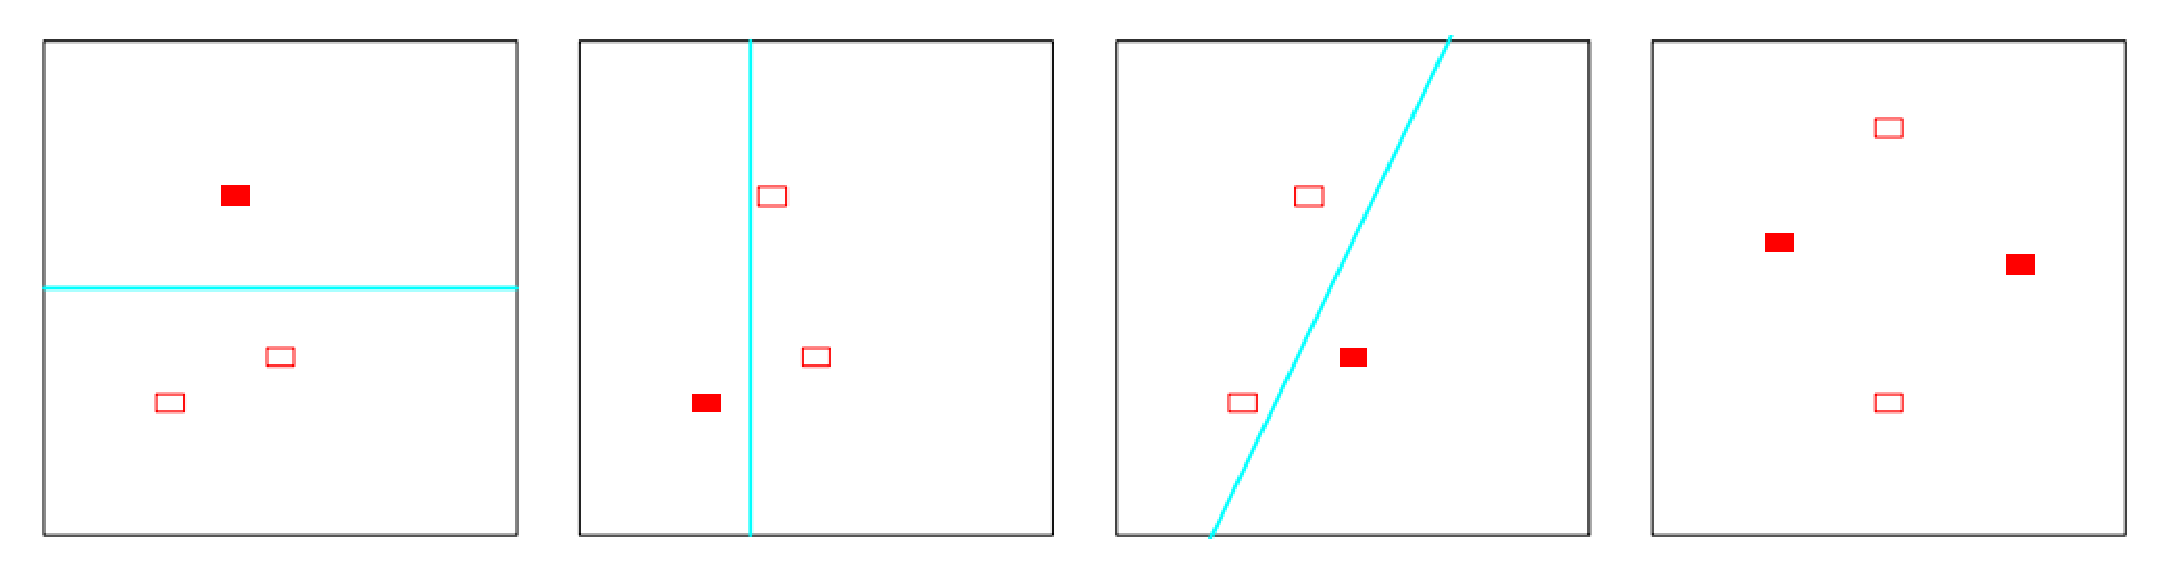
\includegraphics[width=0.85\textwidth]{figures/shatteredset.eps}
  \caption{二维空间线性模型的VC维}\label{fig:vcdimension}
\end{figure}
图例\ref{fig:vcdimension}左侧三个子图:对给定的三个点的点集,无论正负例如何分布,总存在线性模型可以将其精确地分开,线性分类模型可以将此点集碎化。对于四个点的点集,线性模型无法将右侧子图中分布的正负例精确分类,可以推断二维空间上的线性模型的VC 维等于3。根据生长函数可以推断得到相同的结论:对于图中三个点的点集,线性模型的生长函数为$s(\mathcal F,3) = 8 = 2^3$,而对于四个点的点集,生长函数为$s(\mathcal F,4) = 14 < 2^4$,故$V_{\mathcal F} = 3$。

目前尚无计算任意函数集VC维的通用理论,对于一些特殊的函数集,根据定义可以直接确定它们的VC维。比如,$n$维空间上的线性模型的VC维是$h=n+1$;正弦函数集$\{\sin(\omega x)\}$ 的VC 维是$h=\infty$。对于复杂的学习模型,比如人工神经网络,其VC维不仅与网络结构有关,还受学习算法的影响,因此其VC维的确定更加困难。通过理论或实验计算VC 维是目前统计学习理论有待研究的一个重要问题。

\begin{remark}
$\mathcal{F}$俨然是$S$的克星,纵然$S$有那八十二般变化,$\mathcal{F}$总有能人可以见招拆招,一准将其降住。正所谓,道高一尺魔高一丈,$S$ 唯有长叹:既生瑜何生亮,呜呼哀哉!$\mathcal{F}$的法术等级(VC维)可以根据其降服对手的最高等级(势)来确定:降服对手“势力”越强大,则其自身的等级越高。
\end{remark}

\section{期望风险与经验风险}
假设$X$是输入向量空间,$Y$是输出向量空间,乘积空间$Z=X\times Y$存在某种未知的概率分布$P(z) = P(x,y)$,统计学习的目标是从假设空间
$\mathcal F = \{f:X\rightarrow Y\}$中搜索一个最佳函数,使得\textbf{期望风险(Expected Risk)}:
\begin{equation}\label{eq:expectedrisk}
    R_{exp}(f) = \int_{X\times Y}{L(f(x),y)p(x,y)dxdy}
\end{equation}
最小,其中$L$表示损失函数。假设$\hat f$是假设空间中能够对概率分布$P(x,y)$做最佳逼近的函数,那么
\begin{equation}
    \hat f = \arginf\limits_{f\in \mathcal F}R_{exp}(f).
\end{equation}

由于概率分布$P(x,y)$未知,人们只能通过从未知分布中抽取样本集合$S=\{x_i,y_i\}_{i=1}^n$,间接估计出期望风险,这种风险损失又称为\textbf{经验风险}
(Empirical Risk):
\begin{equation}\label{eq:empiricalrisk}
    R_{emp}(f) = \frac{1}{n}\sum_i L(f(x_i),y_i)
\end{equation}
机器学习模型大多是基于经验风险最小化展开:
\begin{equation}\label{eq:slt-er}
    \hat f = \arginf\limits_{f\in \mathcal F} R_{emp}(f)
\end{equation}

通常,经验风险最小化的模型可能过于复杂,比如参数过多,从而产生过拟合问题,不利于模型泛化推广。模型过拟合是不稳定性的一种表现,训练数据集上的微小波动可能给最终训练得到的模型造成根本性的变化。研究表明,确保模型的稳定性,则模型的泛化能力与一致性也能得到保证。通过为经验风险增加一个正则化项,实际上限制了模型选择的范围,降低模型的复杂度,实现结构风险最小化的目的。正则化一般是在经验风险的基础上添加惩罚项:
\begin{equation}\label{eq:regularization}
    \min\limits_{f\in \mathcal F}\frac{1}{n}\sum\limits_i L(f(x_i),y_i) + \lambda \mathcal{R}(f)
\end{equation}
其中,$\mathcal{R}(f)$表示正则化项,$\lambda\ge 0$表示惩罚系数,反映对复杂模型选择的约束力度。

\section{泛化界}
统计学习理论系统地研究了经验风险$R_{emp}$(训练误差)和实际风险$R_{exp}$(期望风险)之间的关系,也即\textbf{泛化界}(Generalization Bound,也称“推广性的界”)。函数集$\mathcal F$的VC维反映了集合中函数的复杂程度,使用VC维可以确定函数$f$的泛化界。假设测试数据与训练数据独立同分布,$\mathcal{F}$ 是二元分类函数集,我们可以使用VC维预测二元分类模型$f\in \mathcal{F}$\textbf{测试误差的概率上界}:
\begin{equation}\label{eq:generalizationbound}
    P\bigg\{R_{exp}(f) \le R_{emp}(f) + \varPhi(n/h)\bigg\} \ge 1 - \eta.
\end{equation}
其中,$n$是训练样本容量,$h$表示函数集$\mathcal F$的VC维,
\[
    \varPhi(n/h) = \sqrt{\frac{h[\ln(2n/h) + 1] - \ln(\eta/4)}{n}}
\]
表示置信范围(或置信误差),$0<\eta<1$表示置信度。
%\begin{equation}\label{eq:testerrorupperbound}
%    R_{emp}(f) \le R_{exp}(f) \le R_{emp}(f) + \sqrt{\frac{h(\ln(2n/h) + 1) - \ln(\eta/4)}{n}} \triangleq  R_{emp}(f) + \varPhi(n/h)
%\end{equation}

如果训练样本有限,VC维$h$越大,则模型越复杂,并且置信范围$\varPhi(n/h)$越大,导致期望风险同经验风险之间的差别越大,从而产生常见的过拟合问题。在机器学习过程中,不仅要控制经验风险,还要控制VC维度以缩小置信范围,实现期望风险最小化,从而取得良好的泛化能力。当无法计算函数集的VC维时,可以采用交叉验证的方法,将样本集分为训练集和验证集,使用训练集样本训练模型,用验证集做测试,并选择验证集上误差最小的模型参数作为训练结果。

泛化界是基于最坏情况下的结论,多数情况下都是松弛的,并且不同模型泛化界的比较只有属于同一类函数集时才是有意义的。

\section{结构风险最小化}
传统的机器学习方法,选择以经验风险最小化作为目标,可能在训练集上可以达到100\%的准确率,但是泛化能力却很弱,执行预测时出现很高的误差。在选择学习模型与算法的过程是在调整置信范围,如果模型与训练样本匹配($h/n$恰当),则可能会取得不错的效果。模型的选择根据经验做出,过分倚重于“技巧”而缺乏理论指导。

统计学习理论给出一种具有指导性的策略:对函数集的子集,按照VC 维大小,即置信范围$\varPhi(h/n)$的大小顺次排列,构成一个函数子集序列:
\begin{equation}\label{eq:funtionalsubset}
    \begin{array}{l}
      \mathcal{F}_1 \subset \mathcal{F}_2 \subset \ldots \subset \mathcal{F}_m \\
      h_1 \le h_2 \le \ldots \le h_m
    \end{array}
\end{equation}
从函数子集中搜索能够最小化经验风险与置信范围之和的子集,实现最小化期望风险,这种思想称作\textbf{结构风险最小化}(Structural Risk Minimization),简称\textbf{SRM准则}。

实现SRM准则有两种思路:一是计算每个子集的最小经验风险,并从中选择经验风险与置信范围之和最小的子集。这种思路计算开销巨大,不可取。二是设计一种特殊的函数集结构,使得每个子集都能够取得最小的经验风险(训练误差为$0$),从中选择置信范围最小的子集。支持向量机正是第二种思想的实现。

%\subsection{Uniform Convergence Theory}

\section{支持向量机分类器}
对于一个包含$n$个样本的训练数据集\[S=\{x_i,y_i\}_{i=1}^n\]其中,$x_i\in \mathbb{R}^m$是样本特征向量,$y_i\in\{-1,1\}$是样本的类标。SVM模型就是求解下面的二次规划问题:
\begin{equation}\label{eq:svm}
    \begin{array}{ll}
      \min\limits_{\omega,b,\xi} & \frac{1}{2}\omega^T\omega + C\sum\limits_{i=1}^n\xi_i\\
      \textit{s.t.} & y_i(\omega^T\phi(x_i) + b) \ge 1 - \xi_i \\
      & \xi_i \ge 0 ,i = 1,2,\ldots,n
    \end{array}
\end{equation}
其中,样本$x_i$经由$\phi$映射到高维特征空间,$\omega$称作超平面法向量,$b$为超平面的截距,$\xi$表示松弛因子,$C >0$是$\ell_1$正则化项(Regularization Term)的惩罚系数。

引入拉格朗日乘子向量$\alpha,\beta \ge 0$,构造拉格朗日函数
\begin{equation}
    L(\omega,b,\xi,\alpha,\beta) = \frac{1}{2} \omega^T \omega + C\sum\limits_{i=1}^n\xi_i - \sum\limits_{i=1}^n \alpha_i \big[y_i(\omega^T\phi(x_i) + b) - 1 + \xi_i\big] - \sum\limits_{i=1}^n \beta_i \xi_i
\end{equation}
若记$\Theta_d(\alpha,\beta) = \min\limits_{\omega,b,\xi} L(\omega,b,\xi,\alpha,\beta)$,由于二次规划\eqref{eq:svm}具有强对偶性,存在全局最优解。一个解是最优解的充要条件是Karush-Kuhn-Tucker条件成立。根据KKT最优解的\textbf{平稳性条件}
\begin{equation}
    \left\{
    \begin{array}{l}
      \frac{\partial L}{\partial \omega} = \omega - \sum\limits_{i=1}^n \alpha_i y_i \phi(x_i) = 0 \\
      \frac{\partial L}{\partial b} = - \sum\limits_{i=1}^n \alpha_i y_i = 0 \\
      \frac{\partial L}{\partial \xi_i}  = C - \alpha_i - \beta_i = 0
    \end{array}
    \right.
\end{equation}
解得最优解$\hat \omega,\hat b,\hat \xi$:
\begin{equation}
    \left\{
    \begin{array}{l}
      \hat \omega = \sum\limits_{i=1}^n \alpha_i y_i \phi(x_i) \\
      \sum\limits_{i=1}^n \alpha_i y_i = 0 \\
      \alpha_i + \beta_i = C
    \end{array}
    \right.
\end{equation}
将其代入拉格朗日函数,整理后得:
\begin{equation}
    \Theta_d(\alpha,\beta) = L(\hat \omega,\hat b,\hat \xi,\alpha,\beta) = \sum\limits_{i=1}^n \alpha_i - \frac{1}{2} \sum\limits_{i=1}^n\sum\limits_{j=1}^n \alpha_i \alpha_j y_i y_j \phi(x_i)^T \phi(x_j)
\end{equation}
与$\beta$完全无关,根据$\alpha_i + \beta_i = C$,\textbf{对偶可行性条件}$\alpha_i\ge 0,\beta_i\ge 0$,可得下面形式的对偶模型:
\begin{equation}\label{eq:dualsvm}
    \begin{array}{ll}
      \max\limits_\alpha & \sum\limits_{i=1}^n \alpha_i - \frac{1}{2} \sum\limits_{i=1}^n \sum\limits_{j=1}^n \alpha_i \alpha_j y_i y_j \phi(x_i)^T \phi(x_j) \\
      \textit{s.t.} & \sum\limits_{i=1}^n \alpha_i y_i = 0 \\
      & 0\le \alpha_i \le C ,i = 1,\ldots,n
    \end{array}
\end{equation}
完全消除了松弛变量对模型的影响。假设对偶模型的最优解是$\hat \alpha,\hat \beta$,根据KKT最优解的\textbf{松弛互补条件}可得
\begin{equation}
    \left\{
    \begin{array}{l}
        \hat \alpha_i \big[y_i(\hat \omega^T \phi(x_i) + \hat b) - 1 + \hat \xi_i \big] = 0\\
        \hat \beta_i \hat \xi_i = 0
    \end{array}
    \right.
\end{equation}
对任意的$i = 1,\ldots,n$成立。由于$\hat \beta_i = C - \hat \alpha_i$
\begin{itemize}
  \item 当$\hat \alpha_i = 0$时,$\hat \beta_i = C$,则$\hat \xi_i=0$,$y_i(\hat \omega^T \phi(x_i) + \hat b) \ge 1$
  \item 当$0 < \hat \alpha_i < C$时,$\hat \beta_i>0$,则$\hat \xi_i=0$,$y_i(\hat \omega^T \phi(x_i) + \hat b) = 1$
  \item 当$\hat \alpha_i = C$时,$\hat \beta_i = 0$,则$\hat \xi_i = 1 - y_i(\hat \omega^T \phi(x_i) + \hat b) \ge 0$,$y_i(\hat \omega^T \phi(x_i) + \hat b) \le 1$
\end{itemize}

SVM从训练集中选择一组特征子集,使得对特征子集的划分等价于对整个数据集的划分,这组特征子集就被称为\textbf{支持向量}(Support Vector)。当$\hat \alpha_i=0$ 时,对应的样本数据是内部点,分类正确且远离最大间隔分类超平面;当$\hat \alpha_i=C$时,对应的样本数据可能分类错误;当$0< \hat \alpha_i < C$ 时,$y_i(\hat \omega^T \phi(x_i) + \hat b) = 1$ 对应的样本数据位于最大间隔边界上,属于支持向量。给定$\hat \alpha$利用$\hat \omega=\sum\limits_i \alpha_i y_i \phi(x_i)$ 可以计算最优的法向量$\hat \alpha$ 与截距$\hat b$。根据SVM 模型在训练数据集上训练出一个最佳超平面分类模型:
\begin{equation}\label{eq:hyperplane}
    f(x) = \sgn(\hat \omega^T \phi(x) + \hat b) = \sgn(\sum_i \hat \alpha_i y_i \phi(x_i)^T \phi(x) + \hat b)
\end{equation}
对于部分$\hat \alpha_i = C$的样本可能分类错误,可应用于异常点检测问题\cite{matic1992computer}。

最大化分类间隔是控制泛化能力的一个举措,也是SVM的一个核心思想。根据统计学习理论\cite{vapnik1982estimation,vapnik2000nature},在$m$维空间中,如果所有样本都分布在半径为$r$的超球内,则满足条件$\|\omega\| \le z$的指示函数集$f(\omega, b) = \sgn(\omega^T x + b)$的VC维$h$有如下上界:
\begin{equation}
    h \le \min~\{\lceil r^2 z^2\rceil, m\} + 1
\end{equation}
实际上最小化$\|\omega\|^2$的目标体现了最小化VC维上界的SRM准则,有利于选择一个泛化能力强的模型。

\section{核方法}
1964年Aizermann等人~\cite{aizerman1964theoretical}在研究势函数方法时最先使用核方法,1992年Vapnik等人~\cite{boser1992training}同时利用核函数与最大间隔超平面,基于结构风险最小化原理提出SVM。核方法是SVM 成功的关键,赋予SVM处理非线性问题的能力。在具体问题中,选择合适的核函数仍然存在许多实际困难。

\begin{definition}[Gram矩阵]
假设$K(x,y)$是$X\times X$上的一个对称函数,对于输入空间$X$上的一组向量$x_1,\ldots,x_n$,则称矩阵$(K(x_i,x_j))_{n\times n}$为函数$K(x,y)$关于向量组$x_1,\ldots,x_n$的Gram矩阵。
\end{definition}

\begin{definition}[核函数与核矩阵]
给定输入空间$X$,对称函数$K:X\times X\mapsto \mathbb R$,如果存在一个希尔伯特特征空间$H$,及$X$到$H$的映射
\begin{equation}
    \phi: X \mapsto H
\end{equation}
使得任意$x,y\in X$,都有
\begin{equation}
    K(x,y) = \phi(x)^T \phi(y)
\end{equation}
则称$K(x,y)$是$X\times X$上的一个\textbf{核函数},$\phi(x)$为映射函数。对于$X$上的一组向量$x_1,\ldots,x_n$,核函数$K(x,y)$ 关于向量组$x_1,\ldots,x_n$的Gram矩阵
\begin{equation}
    K =
    \begin{bmatrix}
    K_{11}& K_{12} & \cdots & K_{1n}\\
    K_{21}& K_{22} & \cdots & K_{2n}\\
    \vdots & \vdots & \ddots & \vdots\\
    K_{n1}& K_{n2} & \cdots & K_{nn}\\
    \end{bmatrix}
\end{equation}
称作\textbf{核矩阵},其中$K_{ij}=K(x_i, x_j)$。
\end{definition}
对于给定的核函数$K(x,y)$,特征空间$H$和映射函数$\phi$的选取并不唯一,可以取不同的特征空间,即便是在同一个特征空间上也可以取不同的映射。通过核函数构造映射函数通常比较复杂,研究人员提出一个重要的问题:不用构造映射函数$\phi(x)$,能否直接判断一个给定的函数$K(x,y)$是不是核函数?换而言之,函数$K(x,y)$满足什么条件时才能成为核函数?

\begin{theorem}[Mercer条件\cite{mercer1909functions}]
对称函数$K:X\times X\mapsto \mathbb{R}$为正定核(或Mercer 核),当且仅当它关于$X$上任意一组向量$x_1,\ldots,x_n$的Gram矩阵$K = [K(x_i,x_j)]_{n\times n}$ 都是半正定(Positive Semi-definitive)矩阵。
\end{theorem}
\begin{proof}
\textbf{必要性}:若$K(x,y)$是$X\times X$上的正定核,则存在映射$\phi:X\mapsto H$,使得
\[
    K(x,y) = \phi(x)^T \phi(y), \forall x,y\in X,
\]
那么,对于任意一组$X$上的向量$x_1,\ldots,x_n$,我们可以根据正定核$K(x,y)$构造对应的Gram矩阵$K=[K_{ij}]_{n\times n} = [K(x_i,x_j)]_{n\times n}$,对任意的$c_i\in \mathbb{R},i=1,\ldots,n$,都有
\begin{equation}
    \sum\limits_{i,j} c_i c_j K(x_i,x_j) = \sum\limits_{i,j} c_i c_j \phi(x)^T \phi(y) = [\sum\limits_i c_i \phi(x_i)]^T[\sum\limits_j c_j\phi(x_j)] = \|\sum\limits_i c_i \phi(x_i)\|^2 \ge 0
\end{equation}
表明核矩阵都是半正定矩阵。

\textbf{充分性}:对于任意的$x_i\in X,i=1,\ldots,n$,函数$K(x,y)$关于$x_1,\ldots,x_n$的Gram 矩阵$K = [K(x_i,x_j)]_{n\times n}$是半正定矩阵。我们使用构造性证明方法,通过三个步骤在函数$K(x,y)$的基础上构造出一个希尔伯特空间$H$、输入空间$X$到希尔伯特空间$H$的一个映射$\phi$:

\noindent \textbf{1、向量空间}:
定义映射$\phi:x\mapsto K(\cdot,x)$,则对任意$x_i\in X,\alpha_i\in \mathbb{R},i=1,\ldots,n$,可以定义线性组合
\begin{equation}
    f(\cdot)=\sum\limits_{i=1}^n \alpha_i K(\cdot,x_i)
\end{equation}
构成集合$S$。由于集合$S$对加法和数乘运算封闭,因此构成向量空间。

\noindent \textbf{2、内积空间}:
对$S$上的任意两个元素
\[
    f(\cdot)=\sum\limits_{i=1}^n \alpha_i K(\cdot,x_i), ~~g(\cdot)=\sum\limits_{j=1}^m \beta_j K(\cdot,y_j)
\]
定义一个二元运算$\times$:
\[
    f\times g = \sum\limits_{i=1}^n \sum\limits_{j=1}^m \alpha_i \beta_j K(x_i,y_j)
\]
可以证明运算$\times$是空间$S$的内积,满足如下五个性质:
\begin{eqnarray}
  (cf)\times g = c(f\times g), \\
  (f+g)\times h = f\times h + g\times h, \\
  f \times g = g\times f, \\
  f\times f \ge 0, \\
  f\times f = 0 \Leftrightarrow f = 0.
\end{eqnarray}
根据函数$K(x,y)$的对称性,容易证明前三个等式。由于
\[
    f\times f = \sum\limits_{i=1}^n \sum\limits_{j=1}^n \alpha_i \alpha_j K(x_i,x_j)
\]
根据Gram矩阵的半正定性可知等式右端非负,从而可证$f\times f\ge 0$。 对于最后一个命题,充分性显然,下面证明必要性。

由于$S$是向量空间,则对任意的$\lambda\in \mathbb{R}$,若$f,g\in S$,则$f + \lambda g\in S$。根据$(f + \lambda g) \times (f + \lambda g) \ge 0$,展开可以得到一个关于$\lambda$ 的二次函数
\[
  f\times f + 2\lambda f\times g + \lambda^2 g\times g \ge 0
\]
由$\lambda$的任意性知
\[(f\times g)^2 \le (f\times f)(g\times g).\]
根据运算$\times$的定义,对任意的$x\in X$都有
\[K(\cdot,x) \times f = \sum\limits_{i=1}^m \alpha_i K(x,x_i) = f(x),\]
从而有
\[f(x)^2 = (K(\cdot,x) \times f)^2 \le [K(\cdot,x) \times K(\cdot,x)](f\times f).\]
如果$f\times f = 0$,则对任意的$x\in X$,都有$f(x)=0$,那么$f=0$。由此可以证明$\times$是向量空间$S$的内积,$S$为一个内积空间。为表述方便,我们统一记
\[f^T g=f\times g = \sum\limits_{i=1}^n \sum\limits_{j=1}^m \alpha_i \beta_j K(x_i,y_j).\]

\noindent \textbf{3、完备的内积空间——希尔伯特空间}:
根据内积空间$S$定义的内积运算可以自然地诱导出范数
\[
    \|f\| = (f^T f)^{1/2}
\]
因此内积空间$S$也是一个赋范空间。根据泛函分析理论,对于不完备的内积空间$S$,一定可以完备化成为希尔伯特空间(完备的内积空间)$H$。对于给定的函数$K(x,y)$,可以构造从$X$到某个希尔伯特空间$H$的映射$\phi:x\mapsto K(\cdot,x)$,并且满足
\[
    K(\cdot,x)^T f=f(x),\qquad K(\cdot,x)^T K(\cdot,y) = K(x,y)
\]
则根据映射定义可知$K(x,y)=\phi(x)^T \phi(y)$,表明$K(x,y)$是$X\times X$上的核函数。
\end{proof}

\begin{definition}[正定核]
如果对称函数$K(x,y)$关于$x_i\in X,i=1,\ldots,n$的Gram矩阵是半正定矩阵,则称它是正定核。
\end{definition}

\begin{corollary}
正定核的非负线性组合仍然是正定核。
\end{corollary}

\begin{definition}[再生核希尔伯特空间]
假设$H$是由函数$f:X\mapsto \mathbb{R}$构成的希尔伯特空间,如果函数$K: X\times X \mapsto \mathbb R$满足\textbf{再生性},对任意$x\in X$都有$K(\cdot,x)\in H$,且对任意$f\in H$都有
\begin{equation}
    f(x) = K(\cdot,x)^T f
\end{equation}
则称$K$是$H$的\textbf{再生核}。如果$H=\overline{span\{K(\cdot,x),x\in X\}}$(或Dirac泛函$\delta_x(f)=f(x)$连续),$\bar A$ 表示集合$A$ 的闭包,则称空间$H$是\textbf{再生核希尔伯特空间}(Reproducing Kernel Hilbert Space, RKHS)。
\end{definition}

\begin{theorem}[表示定理]
Tikhonov正则化问题
\begin{equation}
    \min\limits_{f\in H}~\frac{1}{2} \sum\limits_{i=1}^n L(f(x_i),y) + \frac{1}{2} \lambda\|f\|_K^2
\end{equation}
的解可以写作
\begin{equation}
    f = \sum\limits_{i=1}^n \alpha_i K(\cdot,x_i)
\end{equation}
的形式。其中,$L(\cdot,\cdot)$是损失函数,$\|\cdot\|_K^2$是正则化项,同输入空间$X\times X$上的核函数$K(\cdot,\cdot)$有关。
\end{theorem}

假设核函数$K(x,y)$关于$\{x_1,x_2,\ldots,x_n\}$生成的核矩阵为$K = K^T$,根据表示定理,任选一个向量$x_j$,都有
\begin{equation}
    f(x_j)=\sum\limits_{i=1}^n \alpha_i K(x_i,x_j)=\alpha^T K_j.
\end{equation}
其中,$K_j$表示矩阵$K$的第$j$ 列。由内积定义,我们可以推断知
\begin{equation}
    \|f\|_K^2 = [\sum\limits_{i=1}^n \alpha_i K(\cdot,x_i)]^T [\sum\limits_{i=1}^n \alpha_i K(\cdot,x_i)] = \sum\limits_{i=1}^n \sum\limits_{j=1}^n \alpha_i\alpha_j K(x_i,x_j) = \alpha^T K \alpha.
\end{equation}
如果假设损失函数$L$为平方差损失,则原始Tikhonov正则化问题可等价地写作
\begin{equation}
    \min\limits_{\alpha\in\mathbb{R}^n}~\frac{1}{2} \|K \alpha - y\|^2 + \frac{1}{2} \lambda \alpha^T K \alpha,
\end{equation}
根据极值必要性条件有解
\begin{equation}
    \alpha = (K  + \lambda I)^{-1} y.
\end{equation}
只要正则化因子$\lambda$选择恰当,就可以保证$K + \lambda I$的非奇异/正定性。当使用线性核$K(x,y)=x^T y$时,则$K = X^T X$,问题就转化为岭回归问题:
\begin{equation}
    \alpha = (X^T X  + \lambda I)^{-1} y
\end{equation}
Tikhonov正则化方法有助于控制模型的平滑性,避免欠拟合与过拟合问题。

在机器学习领域,常用的核函数有如下几种:
\begin{enumerate}[(1)]
  \item 线性核函数(Linear Kernel):$K(x,y) = x^T y$
  \item 多项式核函数(Polynomial Kernel):$K(x,y) = (\gamma x^T y + r)^d$
  \item 高斯径向基函数(Gaussian Radial Basis Function, RBF):$K(x,y) = e^{-\|x - y\|^2/2\gamma^2}$
  \item Sigmoid核函数:$K(x,y) = \tanh\{-\gamma x^T y + r\}$
  \footnote{$\tanh x = \frac{e^x - e^{-x}}{e^x + e^{-x}}$}
\end{enumerate}
根据核函数的性质,我们还可以组合多个核函数构成复杂的核函数。

利用标准二次优化技术训练SVM模型有诸多不便,存在模型复杂不易实现、核矩阵的存储与计算开销大、训练速度慢等问题。为了解决训练速度问题,人们提出很多改进算法,包括块算法(Chunking Algorithm)\cite{vapnik1982estimation}、Osuna算法\cite{osuna1997improved}、SMO算法\cite{platt1998sequential}、SVMLight算法
\cite{joachims1999making,joachims2002learning}、Pegasos算法\cite{shalev2007pegasos} 等。

\section{块算法}
由于支持向量机分类模型只与支持向量有关,同其他所有训练样本都无关,如果仅使用支持向量作为训练集,可以训练得到一致的分类模型。1982年,Vladimir Vapnik与Samuel Kotz根据这种思想提出了块算法(Chunking Algorithm)\cite{vapnik1982estimation}。块算法将训练数据集分成两部分:工作样本集与测试样本集,在工作样本集上应用二次规划优化算法,得到由支持向量表示的分类模型,再利用它从余下所有样本中筛选出违反KKT条件的样本,并入支持向量构成新的工作样本集,然后重新训练。根据这种分解策略,如果样本中支持向量数目很少,工作集样本的数目远小于总样本个数,则可以节省大量的训练时间。在实际应用中,支持向量的数目可能很多,随着迭代的不断推进,工作样本集的规模将逐渐扩大,增加了训练的负担。

\section{Osuna分解算法}
1997年,Edgar Osuna等人\cite{osuna1997support,osuna1997improved}提出Osuna分解算法,在每次迭代训练时固定工作样本集(工作集,Working Set)的规模,将非工作集上违反KKT 条件最严重的样本与工作样本集中的样本进行等量交换,无论支持向量数目多大,都不会改变工作样本集的规模。由于Osuna算法涉及到一个工作样本换出问题,换出的工作样本可能是一个支持向量,那么此算法的关键就在于选择一种合适的样本换入换出策略,确保算法能够收敛并且快速地收敛到最优结果。

Osuna算法固定工作集的规模,并假设其规模足以包含所有的支持向量($\alpha_i>0$),同时又不会超出计算机解决子问题的能力范围(内存、计算复杂度)。它将数据集分解成两部分:工作集B与非工作集N,相应地乘子集也分成两部分,保持非工作集对应的乘子不变,在工作集上定义下面形式的子问题:
\begin{equation}
    \begin{array}{ll}
      \max\limits_{\alpha_B} & \Theta(\alpha_B,\alpha_N)\\
      \textit{s.t.} & \sum\limits_{i\in B} \alpha_i y_i + \sum\limits_{i\in N} \alpha_i y_i = 0 \\
      & 0\le \alpha_i \le C ,i\in B
    \end{array}
\end{equation}
根据工作集B与非工作集N,原问题的目标函数可以表示成下面的形式:
\begin{eqnarray}
    \Theta(\alpha_B,\alpha_N) &=&\big[\sum\limits_{i\in B} \alpha_i - \frac{1}{2} \sum\limits_{i\in B} \sum\limits_{j\in B} \alpha_i\alpha_j y_i y_j K_{ij} - \sum\limits_{i\in B}\sum\limits_{j\in N} \alpha_i\alpha_j y_i y_j K_{ij}\big] + \\
   && \big[\sum\limits_{i\in N} \alpha_i - \frac{1}{2} \sum\limits_{i\in N} \sum\limits_{j\in N} \alpha_i\alpha_j y_i y_j K_{ij}\big].
\end{eqnarray}
在子问题中,$\alpha_B$是所有工作集对应乘子构成的列向量,非工作集N上的乘子保持固定为常数,子问题的目标函数可以将其忽略。子问题的规模与非工作集的大小、支持向量的数目无关。

\begin{theorem}[Osuna定理]
如果从工作集B中换出一个变量到非工作集N,则原问题的目标函数值不变,原问题的新解也是子问题的可行解。如果非工作集N中存在一个违反KKT条件的变量,将其换入到工作集B,则重新优化子问题后,原问题的目标函数值严格递增。
\end{theorem}
\begin{proof}
假设从工作集B中换出的样本为$x_v$,则新工作集为$B'=B\setminus \{v\}$,新的非工作集为$N'=N\cup\{v\}$,则有
\begin{equation}
    \begin{array}{ll}
       & \Theta(\alpha_B,\alpha_N) \\
      = & \sum\limits_{i\in B} \alpha_i - \frac{1}{2} \sum\limits_{i\in B} \sum\limits_{j\in B} \alpha_i\alpha_j y_i y_j K_{ij} - \sum\limits_{i\in B}\sum\limits_{j\in N} \alpha_i\alpha_j y_i y_j K_{ij} + \sum\limits_{i\in N} \alpha_i - \frac{1}{2} \sum\limits_{i\in N} \sum\limits_{j\in N} \alpha_i\alpha_j y_i y_j K_{ij}\\
      = & \sum\limits_{i\in B'} \alpha_i - \frac{1}{2} \sum\limits_{i\in B'} \sum\limits_{j\in B'} \alpha_i\alpha_j y_i y_j K_{ij} - \sum\limits_{i\in B'}\sum\limits_{j\in N'} \alpha_i\alpha_j y_i y_j K_{ij} + \sum\limits_{i\in N'} \alpha_i - \frac{1}{2} \sum\limits_{i\in N'} \sum\limits_{j\in N'} \alpha_i\alpha_j y_i y_j K_{ij} \\
      = & \Theta(\alpha_{B'},\alpha_{N'})
    \end{array}
\end{equation}
表明原问题目标函数值不变。对于原问题的新解$(\alpha_{B'},\alpha_{N'})$,满足子问题的等式约束
\begin{equation}
    \sum\limits_{i\in B'} \alpha_i y_i + \sum\limits_{i\in N'} \alpha_i y_i = \sum\limits_{i\in B} \alpha_i y_i + \sum\limits_{i\in N} \alpha_i y_i = 0
\end{equation}
且满足子问题的不等式约束,则新解$\alpha_{B'}$也是子问题的可行解。对于反向操作,我们可以得到相同的结论。

对于非工作集N,如果存在违反KKT条件的样本$x_u$,则它必然满足如下某个条件:
  \begin{equation}
    \left\{
    \begin{array}{ll}
        \alpha_u=0, & y_u [\omega_u^T \phi(x_u) + b] < 1\\
        0<\alpha_u<C, & y_u [\omega_u^T \phi(x_u) + b] \ne 1\\
        \alpha_u=C, & y_u [\omega_u^T \phi(x_u) + b] > 1
    \end{array}
    \right.
  \end{equation}
将其换入到工作集B,显然不会改变原问题的目标函数值,并且原问题的新解对于新的子问题可行。对于工作集$B'$上新的子问题
  \begin{equation}
    \begin{array}{ll}
      \max\limits_{\alpha_{B'}} & \Theta(\alpha_{B'},\alpha_{N'})\\
      \textit{s.t.} & \sum\limits_{i\in B'} \alpha_i y_i + \sum\limits_{i\in N'} \alpha_i y_i = 0 \\
      & 0\le \alpha_i \le C ,i\in B'
    \end{array}
  \end{equation}
经过优化求解以后,必然有
\begin{equation}
    \Theta(\alpha_B,\alpha_N) = \Theta(\alpha_{B'},\alpha_{N'}) \le \max\limits_{\alpha_{B'}}~\Theta(\alpha_{B'},\alpha_{N'})
\end{equation}
能够逐步改善原问题的目标函数值。
\end{proof}

Osuna算法将原问题分解为一系列子问题,通过求解所有子问题实现求解原问题的目的,它包括三个基本步骤:
\begin{itemize}
  \item 从数据集中任意固定数目的样本构成工作集B
  \item 优化求解定义在工作集B上的子问题
  \item 对于非工作集,如果存在违反KKT条件的样本$x_j$,从工作集B中任选一个样本$x_i$与之交换,并优化求解新工作集$B'=B\setminus\{x_i\}\cup\{x_j\}$ 上的子问题
\end{itemize}

由于原问题与子问题都具有凸可行域,并且目标函数为凸二次函数,则目标函数有界,Osuna算法一定可以在有限次迭代后收敛到全局最优解。Osuna算法与块算法的主要区别在于目标函数的构成,Osuna算法包含全部训练样本(工作集与非工作集),目标函数在保持上次迭代结果的基础上,优化新工作集上定义的子问题。块算法每次迭代直接设定工作集以外的拉格朗日乘子为零,收敛效率低且目标函数值并非最优。

\section{序列最小优化算法}
1998年,微软研究院的John Platt\cite{platt1998sequential}提出著名的\textbf{序列最小优化算法}(Sequential Minimal Optimization,简称SMO),可以高效地训练线性SVM模型,易于实现和扩展,尤其适合处理大型稀疏数据。SMO算法吸收Osuna算法的分治思想,\textbf{将二次规划问题分解成一系列存在解析解的最小子问题},通过子问题实现求解原始凸优化问题。2001年,Chih-Jen Lin\cite{lin2001convergence}给出SMO算法严格的收敛性证明。

如果我们将正定核$K(x,y)$引入到模型\eqref{eq:dualsvm},可以得到下面形式的凸优化问题:
\begin{equation}
    \begin{array}{ll}
      \max\limits_\alpha & \Theta(\alpha) = \sum\limits_{i=1}^n \alpha_i - \frac{1}{2} \sum\limits_{i=1}^n \sum\limits_{j=1}^n \alpha_i \alpha_j y_i y_j K_{ij} \\
      \textit{s.t.} & \sum\limits_{i=1}^n \alpha_i y_i = 0 \\
      & 0\le \alpha_i \le C ,i = 1,\ldots,n
    \end{array}
\end{equation}
每个拉格朗日乘子都对应一个训练样本,模型中的不等式约束条件构成典型的凸包。SMO算法与Osuna算法类似,将原始数据集分解成两部分:工作集与非工作集,并且固定工作集的规模至最小。当工作集降至只有一个变量时,根据等式约束条件,工作集对应的乘子变量直接固定,无法实现优化子问题目标函数的目的。SMO算法将工作集固定为两个变量($|B|=2$),根据等式约束与变量界的不等式约束,可以直接通过解析式优化子问题的目标函数。

\subsection{解析方法:优化拉格朗日乘子对}
假定当前满足全部约束条件的拉格朗日乘子向量$\alpha^t$,根据Osuna算法(或坐标上升法)的思想,我们选定工作集为$B=\{i,j\}$。不失一般性,假设$i<j$,则非工作集为$N=\{1,2,\ldots,i-1, i+1,\ldots,j-1,j+1,\ldots,n\}$。在下次迭代时,SMO算法保持非工作集当前状态不变,则目标函数变成一个形式简单的二元二次函数:
\begin{equation}
    \begin{array}{lll}
    \Theta(\alpha) & = & \Theta(\alpha_1^t,\ldots, \alpha_{i-1}^t, \textcolor{red}{\alpha_i},\alpha_{i+1}^t,\ldots,\alpha_{j-1}^t,\textcolor{red}{\alpha_j},\alpha_{j+1}^t,\ldots,\alpha_n^t) \\
    & = & \alpha_i \big[ 1 - y_i \sum\limits_{k\in N} \alpha_k^t y_k K_{ik} \big] + \alpha_j \big[1 - y_j \sum\limits_{k\in N} \alpha_k^t y_k K_{jk}\big]\\
    && - \alpha_i \alpha_j y_i y_j K_{ij} - \frac{1}{2} \alpha_i^2 K_{ii} - \frac{1}{2} \alpha_j^2 K_{jj} + \Theta_N
    \end{array}
\end{equation}
其中$\Theta_N$是只与非工作集N有关,但与$\alpha_i,\alpha_j$无关的常量。根据问题的约束条件,可行域被限定在矩形区域$[0,C]\times[0,C]$ 内的线段上
\begin{equation}
    \alpha_i y_i + \alpha_j y_j = -\sum\limits_{k\in N} \alpha_k^t y_k = \alpha_i^t y_i + \alpha_j^t y_j
\end{equation}
等式两端同时乘以$y_j$可得
\begin{equation}
    \alpha_j = \alpha_j^t + y_i y_j (\alpha_i^t - \alpha_i).
\end{equation}
我们由此将原始的二元目标函数化为一元二次函数,从而获取解析形式的最优解。根据工作集中两个变量的线性关系,以及变量的边界条件
\begin{equation}
    \left\{
    \begin{array}{c}
      0\le \alpha_i \le C \\
      0\le \alpha_j \le C
    \end{array}
    \right.
\end{equation}
可以确定变量$\alpha_j$的范围$[L, H]$:
\begin{itemize}
  \item 当$y_i y_j = 1$时,$\alpha_j = \alpha_j^t + \alpha_i^t - \alpha_i$,则有
      \begin{equation}
        L = \max\{0,\alpha_i^t + \alpha_j^t - C\},\quad H = \min\{C,\alpha_i^t + \alpha_j^t\}
      \end{equation}
  \item 当$y_i y_j = -1$时,$\alpha_j = \alpha_j^t - \alpha_i^t + \alpha_i$,则有
      \begin{equation}
        L = \max\{0,\alpha_j^t - \alpha_i^t\},\quad H = \min\{C,\alpha_j^t-\alpha_i^t+C\}
      \end{equation}
\end{itemize}

\noindent 对于单变量函数,根据极值必要性条件,令一阶导函数$\nabla_j \Theta(\alpha) = 0$,可以算得$\Theta(\alpha)$的无约束最优解
\begin{equation}
    \hat\alpha_j = \alpha_j^t + \frac{y_j(e_i - e_j)}{K_{ii} + K_{jj} - 2 K_{ij}}.
\end{equation}

它由两部分构成,第一部分为上次迭代结果,第二部分
\begin{equation}\label{eq:updatestep}
    \Delta_j = \frac{y_j (e_i - e_j)}{K_{ii} + K_{jj} - 2 K_{ij}}
\end{equation}
可以视为变量$\alpha_j$更新的步长,其中
\begin{equation}
    e_k = \big[\sum\limits_{l=1}^n y_l \alpha_l^t K_{kl} + b\big] - y_k, \quad k = i, j
\end{equation}
表示模型的预测误差。从目标函数的凹凸性来看,一般地都有
\begin{equation}
    \nabla^2_{jj} \Theta(\alpha) = 2 K_{ij} - K_{ii} - K_{jj}  = -\|\phi(x_i) - \phi(x_j)\|^2 < 0,
\end{equation}
表明目标函数在$(-\infty, \hat\alpha_j)$范围单调递增,在$(\hat\alpha_j,\infty)$范围单调递减。由于可行域在$[L,H]$,则$\hat\alpha_j$未必是可行解。为确保目标函数的最优解可行,我们在边界$L$与$H$处作如下处理
\begin{equation}
    \alpha_j^{t+1} = \left\{
    \begin{array}{ll}
      H, & \hat\alpha_j  > H \\
      \hat\alpha_j,  & L \le \hat\alpha_j  \le H \\
      L, & \hat\alpha_j < L
    \end{array}
    \right.
\end{equation}
根据$\alpha_i$与$\alpha_j$的关系可以根据下式更新$\alpha_i^t$
\begin{equation}
    \alpha_i^{t+1} = \alpha_i^t + y_i y_j (\alpha_j^t - \alpha_j^{t+1}).
\end{equation}

如果如果核函数不满足Mercer条件,则可能导致$\eta_{ij} = 2K_{ij} - K_{ii} - K_{jj} >0$。如果数据集中存在多个相同的输入样本,可能出现$\eta_{ij}=0$。 当$\eta_{ij}\ge 0$ 时,需要在可行域线段上逐个验证,确定能够给目标函数带来最大提升的位置。

\textbf{如果$\hat\alpha_j$是可行解,那么可以保证目标函数在更新后有所改善。如果$\hat\alpha_j$不可行,根据边界确定的可行解可能无法保证目标函数的改善,若没有改善,则恢复到上次迭代的结果,重新选择新的工作集,确保目标函数随迭代次数的增加单调递增。}

\subsection{启发式方法:选取拉格朗日乘子对}
根据Osuna定理\cite{osuna1997improved},SMO算法只要在每一步迭代都能够选择优化两个工作样本,在优化前工作集至少包含一个违反KKT条件的样本,就可以保证目标函数稳步提升。算法的收敛性也可以得到保证。为了提高收敛的速度,SMO算法使用启发式的方式选择并联合优化两个工作样本$\alpha_i$与$\alpha_j$:遍历整个样本空间,选出在一定阈值范围$\epsilon>0$内违反KKT条件的样本作为第一个工作样本$\alpha_i$;遍历所有的非边界数据集,选择出最大化更新步长的样本作为第二个工作样本$\alpha_j$(如果非边界数据集为空,则随机选择一个不同于$\alpha_i$的工作样本)。选择$\alpha_i$的工作计算密集,主要开销集中在对样本,尤其是非边界样本上的KKT 条件检验。

KKT条件是凸优化问题收敛的充要条件,当所有样本都满足KKT条件时,就说明算法已经收敛,从而可以终止迭代。在具体实现时,对KKT 条件的检验都存在一定范围的误差$\epsilon>0$,只要样本在阈值范围内满足KKT条件,都认定是样本满足KKT条件。此外,我们通过分析原问题与对偶问题的对偶间隙,可以发现KKT条件的判定法则与最小化对偶间隙优化目标的一致性。

假设原问题的最优目标函数值为$p$,对偶问题的最优目标函数值为$d$,人们称两者之间的差为对偶间隙
\begin{equation}
    \begin{array}{lll}
      \delta & = & p - d \\
       & = & \big(\frac{1}{2} \omega^T \omega + C\sum\limits_{i=1}^n \xi_i\big) - \big(\sum\limits_{i=1}^n \alpha_i - \frac{1}{2} \sum\limits_{i=1}^n \sum\limits_{j=1}^n \alpha_i \alpha_j y_i y_j K_{ij}\big)  \\
       & = & \sum\limits_{i=1}^n \sum\limits_{j=1}^n \alpha_i \alpha_j y_i y_j K_{ij} - \sum\limits_{i=1}^n \alpha_i + C\sum\limits_{i=1}^n \xi_i \\
    \end{array}
\end{equation}
对于任意一个样本$x_i$,我们从对偶间隙中分解出它的贡献
\begin{equation}
    \delta_i = \alpha_i y_i \sum\limits_{j=1}^n \alpha_j y_j K_{ij} - \alpha_i + C\xi_i = \alpha_i (y_i g_i - 1 - y_i b) + C\xi_i
\end{equation}
其中,$g_i = \sum\limits_{j=1}^n \alpha_j y_j K_{ij} + b$。根据KKT条件可知:
\begin{itemize}
  \item 当$\alpha_i = 0$时,$y_i g_i \ge 1$($\xi_i=0$),则$\delta_i =  0$
  \item 当$0 < \alpha_i < C$时,$y_i g_i = 1$($\xi_i=0$),则$\delta_i = \alpha_i (y_i g_i - 1 - y_i b)= - \alpha_i b y_i$
  \item 当$\alpha_i = C$时,$y_i g_i \le 1$($\xi_i = 1 - y_i g_i \ge 0$),则$\delta_i = - b C y_i$
\end{itemize}
其中$0<\alpha_i<C$对应的样本称作\textbf{非边界数据点(Non-bound)},如果样本$x_i$违反了KKT条件:
\begin{itemize}
  \item 当$\alpha_i = 0$时,$y_i g_i < 1$($\xi_i> 0$),则$\delta_i = C\xi_i >0$
  \item 当$0 < \alpha_i < C$时,$y_i g_i > 1$($\xi_i=0$),则$\delta_i = \alpha_i (y_i g_i - 1 - y_i b) > - \alpha_i b y_i$
  \item 当$0 < \alpha_i < C$时,$y_i g_i < 1$($\xi_i= 1 - y_i g_i>0$),则$\delta_i = (C-\alpha_i)(1 - y_i g_i)-\alpha_i b y_i > - \alpha_i b y_i$
  \item 当$\alpha_i = C$时,$y_i g_i > 1$($\xi_i=0$),则$\delta_i = - b C y_i + C (y_i g_i - 1)>- b C y_i $
\end{itemize}
数据集中违反KKT条件的样本,会增大对偶间隙,进而影响到优化算法的收敛速度。在所有的数据样本中,非边界数据点违反KKT条件的可能性最大,为此SMO算法从第二次迭代开始,在选择第一个工作样本时,首先检测非边界数据集是否满足收敛条件。如果所有非边界数据均满足KKT条件,则算法再检测整个数据集以确保所有样本均满足收敛条件。

SMO算法使用启发式的方法选择第一个优化变量$\alpha_i$后,在筛选第二个优化变量$\alpha_j$时,选择的标准是希望$\alpha_j$发生足够大的变化。根据
\eqref{eq:updatestep}可知:
\begin{equation}
    \alpha_j = \argmax\limits_{k\ne i} |\Delta_k| = \argmax\limits_{k\ne i} \frac{|e_i - e_k|}{|\eta_{ik}|}
\end{equation}
由于$|\eta_{ik}|$牵涉到核矩阵的计算,时间开销较大,为此我们近似地选择优化$|e_i - e_k|$,即
\begin{equation}
    \alpha_j = \argmax\limits_{k\ne i} |e_i - e_k|
\end{equation}

\subsection{确定截距}
每次迭代都要重新计算截距$b$,保证$x_i,x_j$满足KKT条件。当$\alpha_i^{t+1}$在界内,即$0<\alpha_i^{t+1}<C$时,则根据KKT条件应当有$y_i g_i^{t+1} = 1$,两边同时乘以$y_i$,整理可得:
\begin{equation}
    \begin{array}{lll}
        y_i & = & g_i^{t+1} \\
            & = & \sum\limits_{k=1}^n \alpha_k^{t+1} y_k K_{ik} + b^{t+1} \\
            & = & \alpha_i^{t+1} y_i K_{ii} + \alpha_j^{t+1} y_j K_{ij} + \sum\limits_{k\in N} \alpha_k^t y_k K_{ik} + b^{t+1}
    \end{array}
\end{equation}
经过$t$次迭代后,模型在$x_i$上的预测误差为
\begin{equation}
    e_i^t = g_i^t - y_i = \alpha_i^t y_i K_{ii} + \alpha_j^t y_j K_{ij} + \sum\limits_{k\in N} \alpha_k^t y_k K_{ik} + b^t - y_i
\end{equation}
从而可以确立截距的更新规则:
\begin{equation}
    b^{t+1} = b^t - e_i^t - (\alpha_i^{t+1} - \alpha_i^t) y_i K_{ii} - (\alpha_j^{t+1} - \alpha_j^t) y_j K_{ij}
\end{equation}
类似地,对于处于界内的$\alpha_j^{t+1}$同样有
\begin{equation}
    b^{t+1} = b^t - e_j^t - (\alpha_i^{t+1} - \alpha_i^t) y_i K_{ij} - (\alpha_j^{t+1} - \alpha_j^t) y_j K_{jj}
\end{equation}
当$\alpha_i^{t+1},\alpha_j^{t+1}$同时处于界内时,以上两个结果相同。当二者均不在界内时,取两种结果的均值。

\subsection{算法加速}
在更新截距时,需要预测误差,我们对所有非边界数据的预测误差建立缓存,以实现增量更新的目的:
\begin{equation}
    \begin{array}{lll}
        e_k^{t+1} - e_k^t & = & \sum\limits_{s=1}^n (\alpha_s^{t+1} - \alpha_s^t) y_s K_{ks} + (b^{t+1} - b^t \\
         & = & (\alpha_i^{t+1} - \alpha_i^t) y_i K_{ki} + (\alpha_j^{t+1} - \alpha_j^t) y_j K_{kj} + (b^{t+1} - b^t)
    \end{array}
\end{equation}
当核函数为线性核时,$K_{ij} = x_i^T x_j$,我们可以利用下式直接更新法向量$\omega$:
\begin{equation}
    \omega^{t+1} = \omega^t + (\alpha_i^{t+1} - \alpha_i^t) y_i x_i + (\alpha_j^{t+1} - \alpha_j^t) y_j x_j
\end{equation}
直接用于预测未知样本的类别,无需遍历整个样本空间作内积运算。

\subsection{终止条件}
SMO算法终止条件可以是当所有训练样本均满足KKT条件,或者目标函数率小于某个阈值$\epsilon$,即
\begin{equation}
    \frac{\Theta(\alpha^{t+1}) - \Theta(\alpha^t)}{\Theta(\alpha^t)} < \epsilon
\end{equation}

\section{SVMLight}
1999年,Thorsten Joachims\cite{joachims1999making,joachims2002learning}改进Osuna算法,提出SVMLight算法。SVMLight算法将训练样本分解成工作样本集B与非工作样本集N,并固定B的规模为一个偶数。在每次迭代中,首先确定B,并求解关于B的二次规划问题,并保持N中的拉格朗日乘子固定。每次优化完成后,使用N中违反KKT条件的样本替换B 中的样本。

SVMLight算法对Osuna算法的改进主要反映在以下几点:1)使用最速可行下降法选择工作集B。2)提出一种Shrinking启发式方法,估计出有界支持向量和非支持向量,有效降低二次规划问题的规模。

\section{LibSVM}
SMO算法将工作样本集的规模将至两个,一个直接后果就是迭代次数的增加。此外,SMO算法使用启发式方法选择工作集(拉格朗日乘子对),导致算法收敛速度缓慢。2005 年,台灣國立大學Rong-En Fan 等人\cite{fan2005working}将SVMLight算法的工作集选择策略应用到SMO算法中,并应用Shrinking方法缩小工作集的搜索范围,提高搜索速度。基于改建算法,他们开发的LibSVM\cite{fan2008liblinear,chang2011libsvm}已经成为一个重要的研究工具。

\section{Pegasos}
2007年,Shai Shalev-Shwartz等人\cite{shalev2007pegasos,shalev2011pegasos}设计了一种在线学习算法:Pegasos,全名\textit{Primal Estimated sub-GrAdient SOlver for SVM},使用迭代的方式求解线性支持向量机中的优化问题。Pegasos算法继承了在线学习算法的简洁与高效,最主要的是它可以保证收敛到最优解。

Pegasos改进了随机梯度算法,使用固定大小的工作集近似计算梯度值。在具体介绍算法之前,我们首先证明一个命题。
\begin{theorem}[\cite{li2012statlearning}]
训练无偏置线性支持向量机模型,需要求解下面形式的优化问题
\begin{equation}\label{eq:opt1}
    \begin{array}{ll}
      \min\limits_{\omega,\xi} & \frac{1}{2}\|\omega\|_2^2 + C\sum\limits_{i=1}^n\xi_i\\
      \textit{s.t.} & y_i \omega^T x_i \ge 1 - \xi_i \\
      & \xi_i \ge 0 ,i = 1,2,\ldots,n
    \end{array}
\end{equation}
与下面形式的无约束优化问题等价:
\begin{equation}\label{eq:opt2}
    \min\limits_{\omega}~ L(S; \omega) = \frac{1}{n} \sum\limits_{i=1}^n \ell(y_i, \omega^T x_i) + \frac{\lambda}{2} \|\omega\|_2^2
\end{equation}
其中,$L(S;\omega)$表示模型在数据集$S$上的经验损失,$\ell(y, \hat y) = \max (0, 1-y \hat y)$为合页损失函数。
\end{theorem}

\begin{proof}
对于集合$U=\{(x_i,y_i) \mid 1-y_i \omega^T x_i=\xi_i\ge 0, i=1,\ldots,n\}$,均满足问题\eqref{eq:opt1}中的约束条件。由于
\begin{equation}
    \ell(y_i, \omega^T x_i) = \max \{0, 1-y_i \omega^T x_i\} = \xi_i \ge 0
\end{equation}
最优化问题\eqref{eq:opt2}可以写作:
\begin{equation}
    \min\limits_{\omega,\xi}~ \frac{1}{n} \sum\limits_{i=1}^n \xi_i + \frac{\lambda}{2} \|\omega\|_2^2
\end{equation}
取$\lambda = 1/(nC)$,则与问题\eqref{eq:opt1}等价。类似地,可以将最优化问题\eqref{eq:opt1}写成问题\eqref{eq:opt2}。
\end{proof}

\begin{algorithm}[htbp]
        \caption{Pegasos算法}
        \begin{algorithmic}
            \REQUIRE ~~训练集S,迭代次数T,因子$\lambda$,子集大小m \\
            \STATE
            \begin{itemize}
              \item 选择初始权重向量$\omega_1\in B=\{\omega\mid \|\omega\| \le 1/\sqrt{\lambda}\}$
            \end{itemize}
            \FOR{$t = 1,\dots, T$}
            \STATE
            \begin{enumerate}
              \item 随机抽样:$S_t\subseteq S$且$|S_t|=m$
              \item 样本过滤:$S_t^{+}=\{(x,y)\in S_t\mid y \omega^T x < 1\}$
              \item 更新学习率:$\eta_t = (t\lambda)^{-1}$
              \item 梯度下降更新:$\hat \omega_t = (1-1/t)\omega_t + \eta_t \sum\limits_{(x,y)\in S_t^{+}} (xy)/m$
              \item 超球面映射:$\omega_{t+1} = \min\big\{1, 1/[\sqrt{\lambda}\|\hat \omega_t\|]\big\} \hat \omega_t$
            \end{enumerate}
            \ENDFOR
            \ENSURE ~~模型$f(\omega_T,x)$
        \end{algorithmic}
\end{algorithm}

Pecasos算法在训练过程中,仅使用大小为$m$的部分数据集$S_t$,在此数据集上的经验损失:
\begin{equation}
    L(\omega, S_t) = \frac{1}{m} \sum\limits_{(x,y)\in S_t} \ell(y,\omega^T x) + \frac{\lambda}{2} \|\omega\|_2^2
\end{equation}
由于损失函数是合页损失,那么第一项只有部分是有效的,取出其中损失大于零的样本构成集合$S_t^{+}$,经验损失函数可重新写作:
\begin{equation}
    L(\omega, S_t) = \frac{1}{m} \sum\limits_{(x,y)\in S_t^{+}} (1- y \omega^T x) + \frac{\lambda}{2} \|\omega\|_2^2
\end{equation}

根据梯度下降法,利用其梯度
\begin{equation}
    \nabla_t = -\frac{1}{m} \sum\limits_{(x,y)\in S_t^{+}} (xy) + \lambda \omega_t
\end{equation}
对于最小化问题,可以使用下面的规则更新模型参数:
\begin{equation}
    \hat \omega_t = \omega_t - \eta_t \nabla_t
\end{equation}
整理得:
\begin{equation}
    \hat \omega_t = (1-\eta_t \lambda)\omega_t + \frac{\eta_t}{m} \sum\limits_{(x,y)\in S_t^{+}} (xy)
\end{equation}

Pegasos算法选择半径为$r$的超球面作为对参数的约束界是有依据的:优化模型\eqref{eq:opt2}的最优解在集合内。Pegasos算法的时间复杂度与数据集大小无关,适合用于大数据处理。实验表明,Pegasos算法远优于Joachims的SVM$^{\textrm{Perf}}$ 算法\cite{joachims2006training}。

\section{邻近支持向量机}
2001年,Glen Fung与Oliv Mangasarian\cite{fung2001proximal}提出一种新的简单分类器,称作邻近支持向量机(Proximal Support Vector Machine,PSVM)。实际上,邻近支持向量机不属于支持向量机的范畴,它利用训练数据集构造出的两个尽可能分离的平行邻近超平面,作为数据分类的标准:将数据点的类别标记为距离两个邻近超平面最近的一个,每个超平面都是一类数据聚集的核心。近邻支持向量机模型可以归结为如下形式的等式约束二次规划问题:
\begin{equation}
    \begin{array}{ll}
      \min\limits_{\omega,b,\xi} & \frac{1}{2} (\omega^T \omega + b^2) + \frac{1}{2} C \xi^T \xi\\
      \textit{s.t.} & \Lambda (A\omega + b e) + \xi = e \\
    \end{array}
\end{equation}
其中,$A\in \mathbb R^{n\times m}$表示训练数据集($n$个$m$维数据样本),$\Lambda\in \mathbb R^{n\times n}$ 是一个对角元为数据类标的对角矩阵,$e\in \mathbb R^n$是元素都等于1的向量,两个邻近超平面通过目标函数中的$\omega^T \omega + b^2$ 项尽可能地隔开。

我们引入拉格朗日乘子$\alpha$,构造拉格朗日函数
\begin{equation}
    L(\omega, b, \xi, \alpha) = \frac{1}{2} (\omega^T \omega + b^2) + \frac{1}{2} C \xi^T \xi - \alpha^T [\Lambda (A\omega + b e) + \xi - e].
\end{equation}

根据KKT最优条件,由参数的一阶导函数构成方程组
\begin{eqnarray}
  \nabla_\omega L &=& \omega - A^T \Lambda \alpha = 0 \\
  \nabla_b L &=& b - e^T \Lambda \alpha = 0\\
  \nabla_\xi L &=& C\xi - \alpha = 0\\
  \nabla_\alpha L &=& \Lambda (A\omega + b e) + \xi - e = 0
\end{eqnarray}
由前三个等式建立$\omega,b,\xi$与对偶变量$\alpha$之间的关系
\begin{eqnarray}
  \omega & = & A^T \Lambda \alpha \\
  b &=& e^T \Lambda \alpha\\
  \xi &=& C^{-1} \alpha\\
\end{eqnarray}
把它们带入最后一个等式可得
\begin{equation}
    \Lambda (A A^T + ee^T )\Lambda \alpha + C^{-1} \alpha = e.
\end{equation}

如果我们记$H = \Lambda (A, -e)$,则有$H H^T = \Lambda (A,-e)(A,-e)^T \Lambda = \Lambda (A A^T + ee^T)\Lambda$,进而可得
\begin{equation}
    \alpha = \big[C^{-1} I + H H^T \big]^{-1} e.
\end{equation}

对于大型训练数据,计算矩阵$HH^T\in \mathbb R^{n\times n}$逆运算量很大。为了降低计算复杂度,我们应用Sherman-Morrison-Woodbury公式
\cite{sherman1949adjustment,sherman1950adjustment,woodbury1950inverting}:
\begin{equation}
    \alpha = C\big[I - H(C^{-1} I + H^T H)^{-1} H^T \big]e,
\end{equation}
可以将矩阵逆的运算降至$\complex ((m+1)\times (m+1))\ll \complex (n\times n)$。

\chapter{人工神经网络}
人工神经网络(Artificial Neural Network, ANN),简称神经网络,是人们模仿生物大脑神经工作机理,建立的一种结构化的动态进化模型。由于神经网络强大的表示、学习能力,已经成为一种典型的机器学习技术,应用到各种学习任务,比如分类、回归等。

神经网络模型中,最基本的元素是神经元(Neuron),模拟的正是生物大脑神经元的行为。神经元之间通过“突触(Synapse)”连通,以实现信息的交互传播。与生物神经元相似,神经网络模型中每个神经元通过“突触”接收其他近邻神经元传递的信号,并对这些综合信号的刺激做出相应的反应,比如为每个神经元设置一个固定的阈值或偏置量(Bias),若有效信号量超过这个阈值,则输出1,否则输出0。

\begin{figure}[htbp]
  \centering
  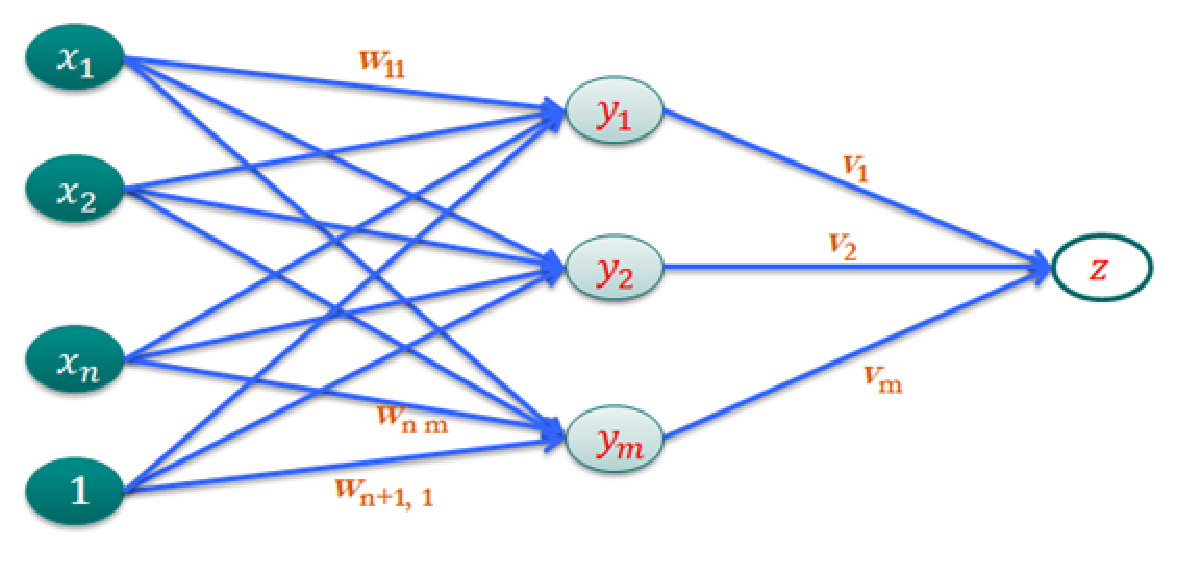
\includegraphics[width=0.65\textwidth,height=6cm]{figures/neuralnetwork.eps}
  \caption{三层神经网络}\label{fig:neuralnetwork}
\end{figure}

典型的神经网络,将神经元划分为三种类型:输入层(Input Layer)、隐藏层(Hidden Layer)、输出层(Output Layer)。每一层都包含多个神经元。输入层主要是用于数据的传递入口;输出层用于输出网络预测的结果;隐藏层是神经网络最吸引人的一层,是神经网络具有强大模拟和学习能力的一个主要因素。
图~\ref{fig:neuralnetwork}是一个典型的三层神经网络,包含$n$个输入神经元,$m$个隐藏神经元,1个输出神经元。箭头方向表示前向传播路径,每一条路径代表一个“突触”,“突触”的权值表示两相邻层神经元关系的重要程度。每个神经元都包含一个激活函数(Activation Function)表示对输入信号的反应,常用的激活函数都是Sigmoid 类型,如Logistic函数,Hyperbolic Tangent函数等。

\section{神经网络简史}
1943年,心理学家Warren McCulloch和数理逻辑学家Walter Pitts\cite{mcculloch1943logical}提出第一个用数理语言描述大脑信息处理过程的计算模型(阈值逻辑或Mcculloch—Pitts神经元),并产生人工神经网络研究的第一次分化:一个方向偏重于生物处理过程,另一个则偏重于神经网络在人工智能方面的应用。
1949年,心理学家Donald Hebb\cite{hebb1968the}提出突触联系可变假设,奠定了神经网络学习算法的研究基础。
1957年,Frank Rosenblatt\cite{rosenblatt1957perceptron} 提出了著名的感知器模型,它是第一个完整的人工神经网络,第一次把神经网络研究付诸工程实现,应用于模式识别、联想记忆等领域,一度有上百家实验室投入研究,美国军方甚至认为神经网络工程比“原子弹工程”更重要,给予巨额资助,并在声纳信号识别等领域取得一定的成绩。
1960年,Bernard Widrow和Marcian Hoff\cite{widrow1960adaptive} 提出自适应线性单元(ADAptive LINear Element, AdaLine),可用于自适应滤波、预测和模式识别,使得人工神经网络的研究进入第一个高潮。
1969年, Marvin Minsky和Seymour Papert\cite{minsky1969perceptron}指出单层感知器表示能力有限,无法处理线性不可分的问题,如异或判断,而多层感知器又过于复杂,按照当时计算机的处理能力根本无法实现。神经网络的研究受此影响,进入长达10年的萧条期。
1982年,Teuvo Kohonen\cite{kohonen1982self}总结大脑神经细胞的自组织特性、记忆方式以及神经细胞兴奋刺激的规律,提出著名的自组织映射(Self-Organizing Map, SOM)理论。
1982年,John Hopfield\cite{hopfield1982neural}用能量函数的思想提出一种新的计算方法,阐明了神经网络与动力学的关系,并用非线性动力学的方法来研究这种神经网络的特性,建立了神经网络稳定性判据,并指出信息存储在网络中神经元之间的连接上,形成了离散Hopfield网络。
1984年\cite{hopfield1984neurons},他又设计与研制了Hopfield网络模型的电路,指出神经元可以用运算放大器来实现,所有神经元的连接可用电子线路来模拟,并称之为连续Hopfield网络。他的研究成果有力推动了神经网络的发展,掀起神经网络研究的又一次热潮。
1984年,David Ackley和Geoffrey Hinton
\footnote{深度学习泰斗、多伦多大学特聘教授、爱丁堡大学人工智能博士,2012年获得加拿大国家最高科学奖,有“加拿大诺贝尔奖”之称的Killam 奖。}
等人\cite{ackley1985learning}将模拟退火算法引入神经网络,提出Boltzmann机网络模型,提供了一种有效的神经网络优化方法。
1986年,Rumelhart等人\cite{rumelhart1986learning}提出了误差反向传播算法(Back Propagation,BP),成为至今为止影响最大的一种网络学习方法。事实上早在1974 年,Paul Werbos\cite{werbos1974beyond}就在博士论文中首次给出了训练一般网络的反向传播学习算法,但一直不为人知。

BP网络存在两种基本的行为:前向传播和反向更新。前向传播表示神经元对信号的传播路径是单向的,从输入层逐层往下一层传播,直至从输出层获取输出信号的过程。反向更新是按照从输出层向隐藏层,从最后一个隐藏层向前一个隐藏层的顺序,从第一个隐藏层向输入层,逐层调整“突触”的权值过程。在监督学习中,反向更新实际上是对前向传播预测偏差的一种反馈和调整,以期达到逐步优化模型的目的。

利用BP算法网络可以从大量的训练样本学习统计规律,从而对未知事件做出预测,具有明显的优越性。90年代,各种机器学习模型相继诞生,如SVM、Boosting、最大熵方法(如逻辑回归)等,它们的结构基本上可以看成是含有单层隐藏节点(SVM、Boosting),甚至没有隐藏节点(逻辑回归)的模型,在小样本和有限计算单元时对复杂函数的表示能力有限,对于复杂问题泛化能力也受到一定制约,因此也被称为\textbf{浅层学习}(Shallow Learning)。

\section{深度学习}
2006年,机器学习领域的泰斗Geoffrey Hinton和他的学生Ruslan Salakhutdinov在《科学》上发表的一篇文章\cite{hinton2006reducing},掀起深度学习的研究浪潮。深度学习通过神经网络模拟人的大脑学习过程,从底层特征中逐层自动学习合并生成具有隐含语义的深层特征,根据大脑的多层抽象机制实现对数据(音频、图片和文本等)的抽象表达。深度学习已经在多个应用人工智能领域,如语音识别(Speech Recognition)、计算机视觉(Computer Vision)和自然语言处理(Nature Language Processing,NLP)取得重大进展,学术研究成果已经成功地应用到产业化流程,诞生了Siri、Android语音识别系统。

2012年,Google在透漏的技术路线图中明确表示要将下一阶段的技术重心放到\textbf{深度学习与知识图谱}(Knowledge Graph)。2012年6月,《纽约时报》披露了Google Brain项目,由斯坦福大学机器学习教授Andrew Ng和大规模计算机系统专家Jeff Dean共同主导,Google Brain使用16,000个CPU Core的并行计算平台模拟神经网络系统,在语音识别和图像识别等领域获得了巨大的成功。2012年12月,Hinton教授在多伦多大学的研究团队使用卷积神经网络深度学习系统,参加被誉为计算机视觉圣杯的ImageNet 大赛并大比分(16\% v.s. 26\%)领先。2013 年3 月,Google收购Hinton团队创立的DNNResearch
\footnote{DNNResearch是一家专注于语音和图像识别技术的研究公司。},
改善Google 图片搜索质量。2013年7月31日,Google发布用于自然语言处理的word2vec。2013年1月,百度成立深度学习研究院(Institute of Deep Learning,IDL),前Facebook资深科学家徐伟、人工智能领域专家余凯、美国新泽西州立大学统计系教授张潼、前AMD 异构计算专家吴韧陆续加盟百度IDL。2013年12月,Facebook成立人工智能实验室,并聘请Yann LeCun
\footnote{深度学习大拿,Hinton教授多伦多大学的博士后,纽约大学终身教授,纽约大学数据科学中心负责人。他在巴黎第六大学(也称皮埃尔玛丽居里大学)Paris VI (Universit\'{e} Pierre et Marie Curie)获得计算机科学博士学位,期间提出反向传播算法。在加盟Facebook之前,他已经在贝尔实验室工作20多年,期间使用卷积神经网络CNN开发出一套手写数字识别系统LeNet,拥有14项发明专利。}
教授坐镇指导。与LeCun一起加入的还有纽约大学计算机科学系副教授Rob Fergus,他的学生Matthew Zeiler 创立一家专门提供图像搜索服务的公司Clarifai,其研发的深度学习算法在2013年ImageNet大赛保持领先。2013 年12月13日,Mark Zuckerburg 与俄罗斯富豪Yuri Milner 出资300万美元设立Breakthrough Prize in Mathematics奖项。

传统的神经网络采用反向传播方式进行,利用迭代算法训练整个网络:随机设定初值,计算当前网络的输出,根据它与真实标签间的差异反向更新网络各层参数,直至收敛。深度学习为克服神经网络训练速度慢、容易过拟合的问题,采用迥然不同的逐层(Layer-wise)训练机制,从而避免深层反向传播误差校正信号减弱,出现梯度扩散
(Gradient Diffusion)现象。

一般地,信号处理(以图像处理为例)都包括以下几个流程(见图\ref{fig:featurelearning}):
\begin{itemize}
    \item 预处理:对输入图像放缩、去噪、背景差分等。
    \item 特征处理:在预处理后的数据上进行特征提取、特征选择、特征降维等工作。
    \item 模型训练:根据图像的特征向量,学习和训练模型。
\end{itemize}
通常,前两步统称为“特征学习”。
\begin{figure}[htbp]
  \centering
  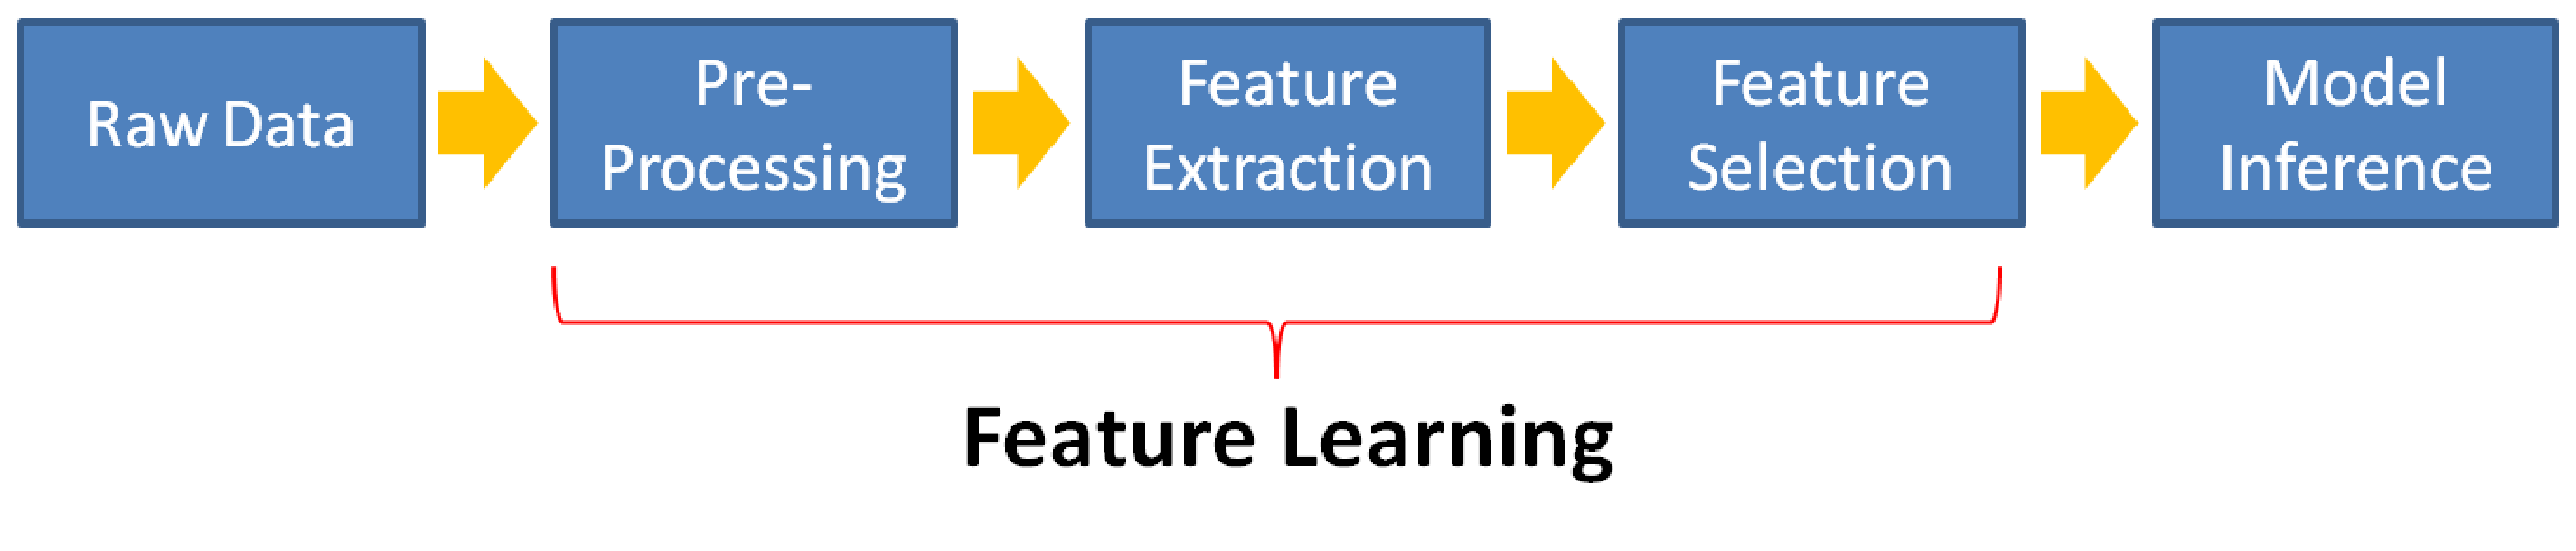
\includegraphics[width=0.85\textwidth,height=2cm]{figures/featurelearning.eps}
  \caption{信号处理流程}\label{fig:featurelearning}
\end{figure}
在流程图中我们看出,后续操作均建立在前面输出结果的基础之上,越是靠前的处理愈加重要,不考虑预处理,特征提取是其中最为重要的部分。特征提取需要大量的人工参与,既增加了特征的不确定性,也产生了大量人力开销。研究人员期望直接从原始数据中学习特征,于是发展出深度学习的概念,距离人工智能的目标又近了一步。深度学习的“无监督特征学习”、“特征学习”之别称由此得名。

假设一个系统$S$有$n$层$S_1,S_2,\ldots,S_n$,系统输入是$I$,输出为$O$,形象地我们可以将其表示成:
\begin{equation}
    I \Rightarrow S_1 \Rightarrow S_2\Rightarrow \cdots \Rightarrow S_n \Rightarrow O
\end{equation}
如果$O=I$,即输入$I$经过系统变化后无任何信息损失,则意味着经过每一层$S_i$,输入$I$都没有任何信息损失,$S_i$可看做原有输入信息$I$的另一种表示。假设有一组输入,并设计了系统$S$,通过调整系统中的参数,使得系统输出$O=I$,由此可自动地获取输入$I$的一系列层次的特征表示$S_1,S_2,\ldots,S_n$。

深度学习常用的方法有Auto Encoder、Sparse Coding和受限Boltzmann机,我们将在后文陆续介绍。

\subsection{自动编码器}
人工神经网络自身就是具有层次结构的系统,给定一个神经网络,假设其输出与输入是相同的,通过训练、调整参数,可以确定每层的权重,代表输入$I$的一层表示。将输入$I$ 的多层表示作为新的特征添加到原始特征中,实验表明有利于改善模型的预测精度,在分类问题中甚至比目前最好的分类算法效果还要好。我们所描述的这种方法称为自动编码器(Auto Encoder)。如果在自动编码器的基础上添加约束性条件,如$\ell_1-$规则化约束,就是“稀疏的自动编码器”方法。

\subsection{稀疏编码方法}
“输出$O$严格地等于输入$I$”的限制略微放松,比如只要二者的差别尽可能地小,由此衍生出一类方法,即稀疏编码(Sparse Coding)方法。假设$b_1,\ldots,b_n$ 是基,输出$O$使用基线性表示:
\[
    O = \sum\limits_{i=1}^n \omega_i b_i
\]
其中,$\omega_i$是基$b_i$的系数,则我们可以得到下面形式的优化问题:
\begin{equation}\label{eq:sparsecode}
    \begin{array}{ll}
      \min\limits_{\omega,b} & \|I-O\|
    \end{array}
\end{equation}
通过解决最小化问题,得到最优的系数与基,它们就是输入$I$的一种近似表达,可以作为特征表示输入。如果对问题\eqref{eq:sparsecode}添加$\ell_1-$规则项:
\begin{equation}\label{eq:regsparsecode}
    \begin{array}{ll}
      \min\limits_{\omega,b} & \|I-O\| + \lambda\sum\limits_{i=1}^n |\omega_i|
    \end{array}
\end{equation}
将一个信号表示为一组基的线性组合,只需要较少的几个基即可近似表示原始信号。

\subsection{玻尔兹曼机}
神经网络是由大量神经元组成的动力学系统。从宏观上看,各神经元的状态可看作是一个随机变量,正如统计物理学中,把大量气体分子看作一个系统,每个分子状态服从统计规律。从统计观点分析,也可寻找神经网络系统中某种神经元的状态的概率分布,分布的形式与网络的结构有关,其参数则是权系数。Hinton等人~\cite{hinton1983optimal}借助统计物理学的方法提出了玻尔兹曼模型,可用于模式分类、预测、组合优化及规划等方面。

1986年,Hinton和Sejnowski~\cite{hinton1986learning}发展出受限玻尔兹曼机(Restricted Boltzmann Machine, RBM),成为机器学习的一个重要工具。RBM属于
\textbf{生成型随机神经网络模型},同普通神经网络类似,包括三层结构:输入层、输出层与隐藏层,由于输入层与输出层可见,称作可见单元(Visible Units),对应地称隐藏层为隐藏单元(Hidden Units)。在图\ref{fig:rbm}中,玻尔兹曼机含有12个可见单元(构成向量$v$)和3个隐藏单元(构成向量$h$)。RBM网络的每一对神经元之间的进行双向对称的信息传递,权值矩阵$W=(w_{ij})$对称,并且自身无反馈$w_{ii}=0$。在RBM网络图上,可见变量与隐藏变量均是二元变量,状态取值范围是$\{0,1\}$。
\begin{figure}[htbp]
  \centering
  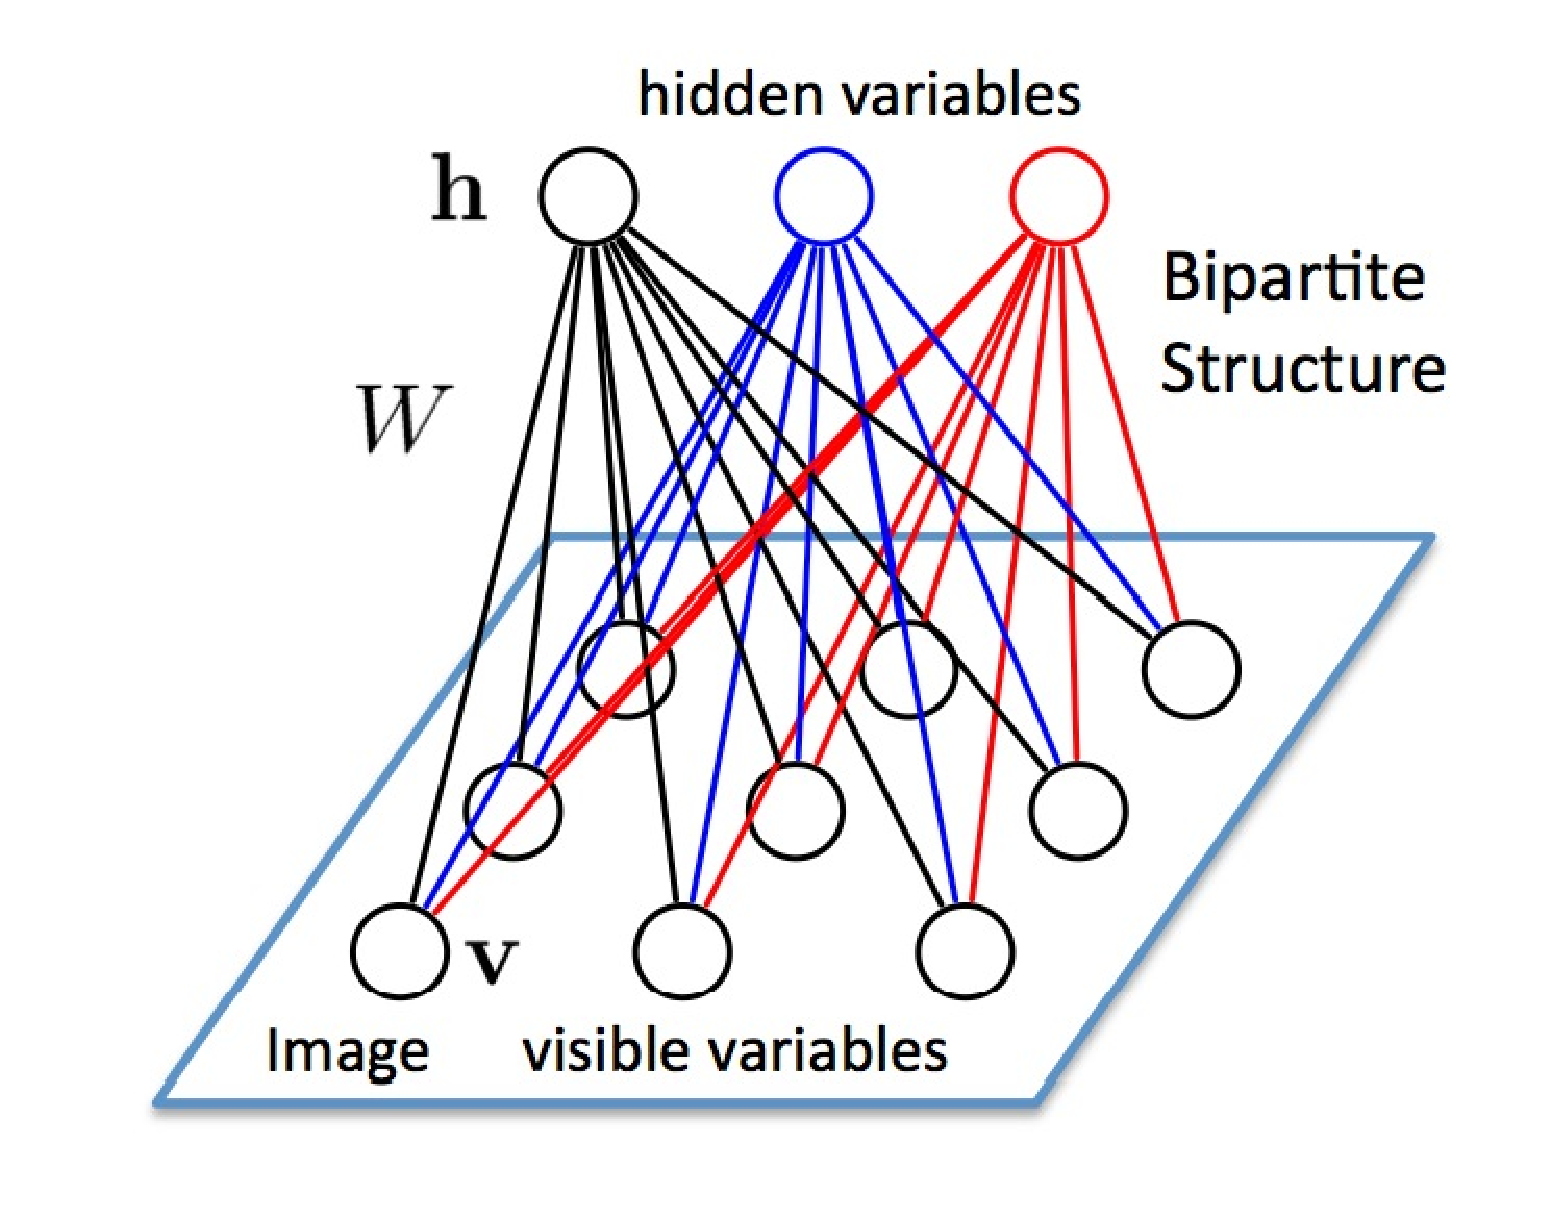
\includegraphics[width=0.5\textwidth, height=5cm]{figures/rbm.eps}
  \caption{受限Boltzmann机}\label{fig:rbm}
\end{figure}

RBM对网络配置$(v,h;\theta)$定义了能量的概念,数学表示如下:
\begin{equation}\label{eq:rbm-energy}
    E(v,h;\theta) = - \sum\limits_{i}\sum\limits_{j} w_{ij} v_i h_j - \sum\limits_{i} a_i v_i - \sum\limits_{j} b_j h_j
\end{equation}
其中,$a_i,b_j$分别表示可见单元$v_i$,隐藏单元$h_j$的偏置权重,$\theta$表示网络参数集。

根据配置能量的定义,RBM给出下面形式的网络配置概率分布
\begin{equation}
    P_{\theta}(v,h) = \frac{1}{Z(\theta)} \exp\big(-E(v,h;\theta)\big)
\end{equation}
其中,$Z(\theta)$表示归一化因子,也称\textbf{配分函数}(Partition Function)。将式子~\eqref{eq:rbm-energy}代入概率分布,可得:
\begin{equation}\label{eq:rbm-distribution}
    P_{\theta}(v,h) = \frac{1}{Z(\theta)} \exp\big(\sum\limits_{i}\sum\limits_{j} w_{ij} v_i h_j + \sum\limits_{i} a_i v_i + \sum\limits_{j} b_j h_j\big)
\end{equation}
对隐藏层上所有可能的配置加和,可计算观测数据的似然函数
\begin{equation}
    P_{\theta}(v) = \frac{1}{Z'(\theta)} \sum\limits_{h} \exp\big(v^T W h + a^T v + b^T h\big)
\end{equation}
并构造对数似然估计函数
\begin{equation}\label{eq:likelihood-estimation}
    L(\theta) = \frac{1}{|V|} \log(\prod\limits_{v\in V} P_{\theta}(v)) = \frac{1}{|V|} \sum\limits_{v\in V} \log(P_{\theta}(v)).
\end{equation}
其中,
\[
    Z'(\theta) = \sum\limits_{v} \sum\limits_{h} \exp\big(v^T W h + a^T v + b^T h\big)
\]
表示归一化项。根据最大似然估计方法,计算对数似然函数的梯度
\begin{equation}
    \begin{array}{lll}
      \partial L(\theta)/\partial w_{ij} & = & \frac{1}{|V|}  \sum\limits_{v\in V} \partial \log(P_{\theta}(v))/\partial w_{ij} = \frac{1}{|V|} \sum\limits_{v\in V} \frac{1}{P_{\theta}(v)} \frac{\partial P_{\theta}(v)}{\partial w_{ij}} \\
       & = & \frac{1}{|V|} \sum\limits_{v\in V} \frac{1}{P_{\theta}(v) Z'(\theta)} \big\{\sum\limits_{h} \exp\big(v^T W h + a^T v + b^T h\big) v_i h_j - P_{\theta}(v) \frac{\partial Z'(\theta)}{\partial w_{ij}} \big\}
   \end{array}
\end{equation}
由于
\begin{equation}
    \partial Z'(\theta)/\partial w_{ij} = \sum\limits_{v} \sum\limits_{h} \exp\big(v^T W h + a^T v + b^T h\big) v_i h_j
\end{equation}
若记
\begin{equation}
    P'_{\theta} = \frac{\exp\big(v^T W h + a^T v + b^T h\big)}{\sum\limits_{h} \exp\big(v^T W h + a^T v + b^T h\big)} = \frac{\exp\big(v^T W h + a^T v + b^T h\big)}{P_{\theta}(v) Z'(\theta)}
\end{equation}
则有
\begin{equation}
    \begin{array}{lll}
      \frac{\partial L(\theta)}{\partial W_{ij}} & = & \frac{1}{|V|} \sum\limits_{v\in V} \bigg[P'_{\theta} v_i h_j - P_{\theta}v^T h\bigg] \\
      & = & \mathbb{E}_{P'_{\theta}} (v_i h_j) - \mathbb{E}_{P_{\theta}} (v_i h_j)
   \end{array}
\end{equation}
成立。由于计算开销较大,Hinton~\cite{hinton2002training}提出了一种高效的学习算法:\textbf{对比散列}(Contrastive Divergence, CD)。

如果增加受限玻尔兹曼机隐藏层的层数,就是\textbf{深度玻尔兹曼}(DBM)。如果在靠近可视层处使用\textbf{贝叶斯信念网络}(Bayisian Belief Network,BBN,表示有向图模型),在离可视层最远处使用受限玻尔兹曼机,就是\textbf{深度信念网络}(Deep Belief Network,DBN)。

\section{信念网络}
1985年,Judea Pearl提出贝叶斯网络,也称信念网络(Belief Network)。它是一种模拟人类推理过程中因果关系的不确定性处理模型,其网络拓朴结构是一个有向无环图(Directed Acyclic Graphic, DAG)。它的节点用随机变量或命题来标识,认为有直接关系的命题或变量则用弧来连接。

\section{卷积神经网络}
卷积神经网络(Convolutional Neural Networks, CNN)是一种特殊的深层神经网络模型,网络中神经元并非完全连接,同一层部分神经元之间共享连接权重。卷积神经网络稀疏连接(Sparse Connectivity)和权值共享(Shared Weights)的结构特性更接近生物神经网络,有效降低了网络模型的复杂度。

CNN源于视觉神经机制,为识别二维图形而设计出的一种多层感知器,对平移、比例缩放、倾斜或其他形式的变形具有高度不变性。1962 年,David Hubel和Torsten Wiesel 研究猫视觉皮层细胞时,提出了感受野(Receptive Field)概念;1984年,日本学者Kunihiko Fukushima基于感受野提出神经认知机(Neocognitron)模型。神经认知机将一个视觉模式分解成多个子模式(特征),进入分层递阶式相连的特征平面进行处理,在物体发生位移或轻微变形时,也能进行识别。神经认知机模型是第一个CNN模型,后来成功应用到手写数字识别、车牌识别和人脸识别等领域。

\chapter{极限学习机}
2006年,Huang Guang-Bin等人\cite{huang2006extreme}在单隐层前向神经网络(Single Hidden Layer Feed-forward Neural Networks,SLFNs)基础上提出一种高效的学习方法,称作\textbf{极限学习机}(Extreme Learning Machine,ELM)。

在传统的神经网络模型中,所有网络中的参数都需要调整,不同层之间存在相互依赖关系。对于前向神经网络模型中,主要使用梯度下降法调整模型参数。梯度下降法存在一个比较常见的问题,迭代步长设置的太小则收敛速度放慢,设置的太大则容易陷入局部最优点。ELM算法不需要调整所有的参数,它随机产生隐藏层权值(输入与隐藏层),并通过解矩阵的广义逆确定输出权值(隐藏层与输出层)。

给定任意$N$个训练样本$(x_i,y_i)$,$i=1,2,\ldots,N$,$x_i\in \mathbb R^n$为输入向量,$y_i\in \mathbb R^m$表示输出向量。对于标准的存在$L$个隐藏节点的前向神经网络模型可以表示成下面形式的数学模型:
\begin{equation}
    f(x) = \sum\limits_{i=1}^L \beta_i g_i(x) = \sum\limits_{i=1}^l \beta_i g(\omega_i^T x + b_i)\in \mathbb R^m
\end{equation}
对于第$i$个隐藏节点,它与输入节点的链接权值向量为$\omega_i\in \mathbb R^n$,它的偏置量(阈值)为$b_i$,它与输出节点链接权值向量为$\beta_i \in \mathbb R^n$,隐藏层的激活函数为$g$,输出层的激活函数是线性函数。给定输入$x\in \mathbb R^n$,模型的第$j$维输出为
\begin{equation}
    f_j(x) = \sum\limits_{i=1}^L \beta_{ij} g_i(x),\quad j = 1,2,\ldots,m.
\end{equation}
对于$N$个输入样本,我们使用向量形式表示单层前向神经网络模型:
\begin{equation}
    f(X) = H \beta
\end{equation}
其中,$H$称作神经网络的隐藏层输出矩阵,具体地
\begin{equation}
    H =
    \begin{bmatrix}
    g(\omega_1^T x_1 + b_1) & g(\omega_2^T x_1 + b_2) & \ldots & g(\omega_L^T x_1 + b_L)\\
    g(\omega_1^T x_2 + b_1) & g(\omega_2^T x_2 + b_2) & \ldots & g(\omega_L^T x_2 + b_L)\\
    \vdots & \vdots & \ddots & \vdots\\
    g(\omega_1^T x_N + b_1) & g(\omega_2^T x_N + b_2) & \ldots & g(\omega_L^T x_N + b_L)\\
    \end{bmatrix}
\end{equation}
如果隐藏层激活函数在任何区间都是无限次可微(Infinitely Differentiable),那么对于任意$N$个不同的输入样本$(x_i,y_i)$,对于任意随机生成的$\omega_i$ 与$b_i$,隐藏层输出矩阵$H$都是可逆矩阵\cite{huang2006extreme}。SLFN模型可以零误差逼近$N$个输入样本,即满足
\begin{equation}
    H\beta = Y.
\end{equation}
传统神经网络模型大多都是基于梯度下降法调整模型参数,SLFN模型随机选择参数$\omega$与$b$,并通过求解最小范数最小二乘问题
\begin{equation}
    \min\limits_{\beta}~\|H\beta - Y\|
\end{equation}
确定Moore-Penrose广义逆表示的最优解
\begin{equation}
    \hat \beta = H^{\dag} Y.
\end{equation}

为了处理分类问题,ELM建立下面形式的优化模型
\begin{equation}
    \begin{array}{ll}
    \min\limits_{\beta,\xi} & \frac{1}{2} \beta^T \beta + \frac{1}{2} C \sum\limits_{i=1}^N \xi_i^T \xi_i\\
    \textit{s.t.} & h(x_i) \beta = y_i^T - \xi_i^T,i = 1,2,\ldots,N
    \end{array}
\end{equation}
建立拉格朗日函数
\begin{equation}
    L(\beta, \xi, \lambda) = \frac{1}{2} \beta^T \beta + \frac{1}{2} C \sum\limits_{i=1}^N \xi_i^T \xi_i - \sum\limits_{i=1}^N \lambda_i (h(x_i) \beta - y_i^T + \xi_i^T)
\end{equation}
根据KKT条件可以得到优化模型的解析解:
\begin{equation}
    \beta = H^T (C^{-1} I + HH^T)^{-1} Y,
\end{equation}
以及输出模型
\begin{equation}
    f(x) = h(x) H^T (C^{-1} I + HH^T)^{-1} Y,
\end{equation}
将其应用于多元分类,我们可以得到决策模型
\begin{equation}
    \hat y_x = \argmax\limits_{i\in\{1,\ldots,m\}} f_i(x).
\end{equation}

\chapter{决策树}
决策树是一种重要的数据表示、决策分析和预测技术,常用于辅助分析决策,学习构造决策模型,在运筹学、数据挖掘、机器学习领域中应用广泛。决策树的优点包括直观易懂、预测准确率高、稳定性好,决策树的成长不需要任何领域知识或参数设置,适用于探索式的知识发现应用。

每一颗决策树都有根节点、内部节点、叶子节点,及连接节点的树枝。如果使用决策树表示一个预测模型,那么根节点表示全部数据集合,每个内部节点表示样本的一个属性,每根树枝则代表对属性的一种判断(测试)结果,每个叶子节点对应一个决策目标(类别标签)。沿着树根到达任意一个叶子节点所经过的路径,就是一个决策(预测)规则。我们在这一节主要介绍和讨论用于数据挖掘的决策树方法。

最早的决策树算法是由Hunt等人\cite{hunt1966experiments}于1966 年提出的概念学习系统(Concept Learning System,CLS)。目前最具影响的是John Quinlan提出的ID3 算法\cite{quinlan1986induction}与C4.5算法\cite{quinlan1993c4}。ID3 算法的目的在于减少树的深度,但忽略了叶子数目的研究。C4.5算法在ID3 算法的基础上进行了改进,对于预测变量的缺值处理、剪枝技术等方面作了较大改进,既适合于分类问题,又适合于回归问题。根据决策树预测结果的数据类型,可以将决策树分成:分类树和回归树,前者预测的是离散型数据,而后者预测的是连续型数据,并且两类决策树的生成方式也不同。ID3与C4.5是两个典型的决策树分类算法,在数据挖掘与机器学习领域还存在其他一些著名的决策树算法,如1980年Gordon Kass\cite{kass1980exploratory}在其博士论文中提出的卡方自动交互检测算法(CHi-squared Automatic Interaction Detection,\textbf{CHAID}),1984年Leo Breiman等人\cite{breiman1993classification}提出的分类回归树(Classification And Regression Tree,\textbf{CART}),1991年Jerome Friedman\cite{friedman1991multivariate}发展的多元自适应回归样条模型(Multivariate Adaptive Regression Splines,\textbf{MARS})。

决策树的生长是一个自顶向下,分而治之的递归过程,在数据集$S$ 上,树的生长基本流程如下:
\begin{itemize}
  \item 如果$S$中所有样本都属于同一类或满足其他停止生长准则,则$S$不再划分,生成叶子节点。
  \item 否则,根据一个指标选择合适的属性与分裂节点,对$S$进行划分,产生多个样本子集$S_i,i=1,2,\dots$,并对每个样本子集$S_i$执行以上两步。
\end{itemize}
在决策树的生长过程,每步选择一个变量对样本做\textbf{最佳划分},衡量划分质量的性能指标,包括ID3算法使用的信息增益、C4.5 使用的信息增益率、CART 算法使用的Gini混杂度(Gini Impurity, GI)和CHAID算法使用的$\chi$值。

\begin{example}
Gore Forest是一家高尔夫俱乐部的经理,他希望通过天气预测人们是否打高尔夫球,以适时调整雇员数量减少开支。为此,他记录了两周内天气情况与高尔夫运动的统计数据(见表~\ref{tbl:golf})。记录的数据中,天气状况包括Outlook(sunny,overcast,rain),Temperature(64--85),Humidity(65--96),Windy
(yes,no)四个变量;类标变量是二元的,表示人们是否打高尔夫。根据统计数据,我们可以构建如图~\ref{fig:decisiontree}所示二元分类决策树模型。
\begin{table}[htbp]
    \centering
    \begin{tabular}{|l|c|c|c|c|c|}
      \hline
        Outlook & Temperature & Humidity & Windy & Play\\
        \hline
        sunny & 85 & 85 & no & no\\
        \hline
        sunny & 80 & 90 & yes & no\\
        \hline
        overcast & 83 & 78 & no & yes\\
        \hline
        rain & 70 & 96 & no & yes\\
        \hline
        rain & 68 & 80 & no & yes\\
        \hline
        rain & 65 & 70 & yes & no\\
        \hline
        overcast & 64 & 65 & yes & yes\\
        \hline
        sunny & 72 & 95 & no & no\\
        \hline
        sunny & 69 & 70 & no & yes\\
        \hline
        rain & 75 & 80 & no & yes\\
        \hline
        sunny & 75 & 70 & yes & yes\\
        \hline
        overcast & 72 & 90 & yes & yes\\
        \hline
        overcast & 81 & 75 & no & yes\\
        \hline
        rain & 71 & 80 & yes & no\\
      \hline
    \end{tabular}
    \caption{天气状况与高尔夫运动状况关联表}
    \label{tbl:golf}
\end{table}

\begin{figure}[htbp]
  \centering
  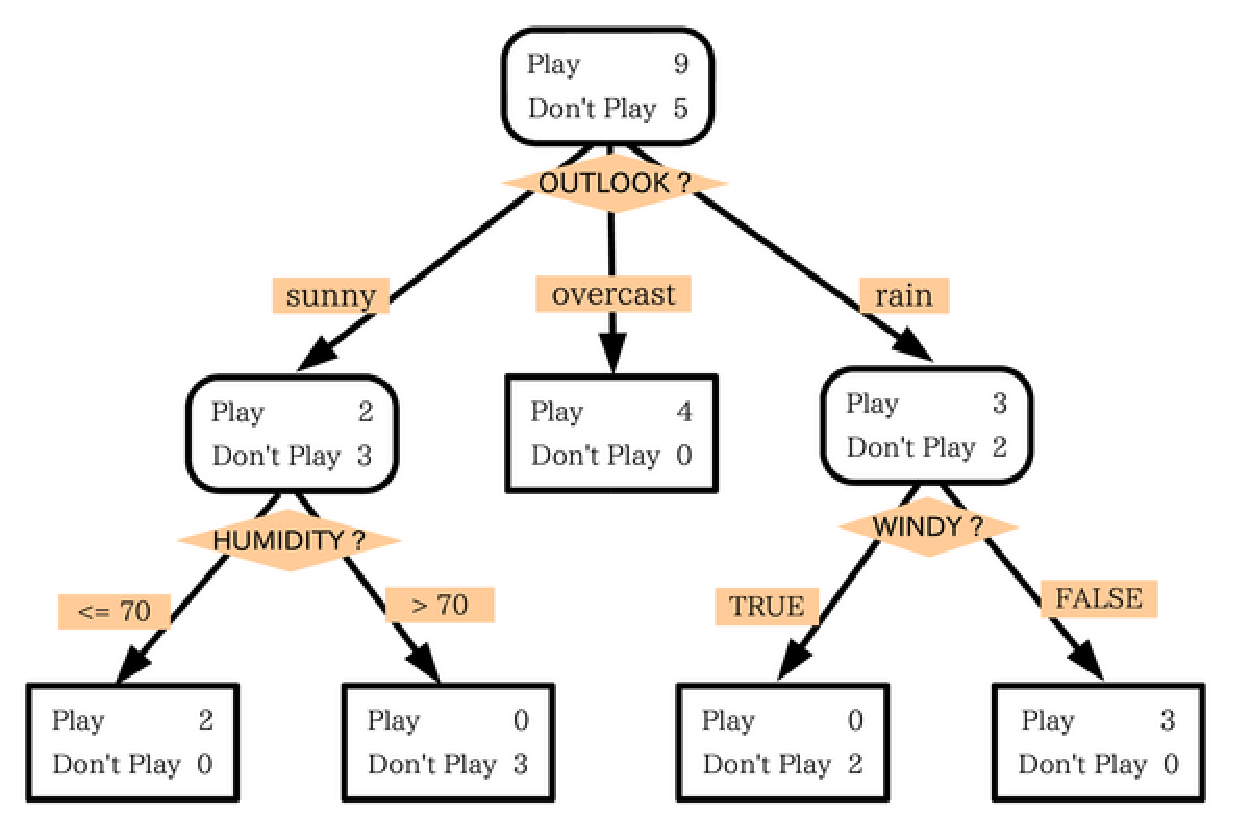
\includegraphics[width=0.85\textwidth]{figures/decisiontree.eps}
  \caption{决策树预测模型}\label{fig:decisiontree}
\end{figure}

\end{example}

\subsection{决策树桩}
决策树桩(Decision Stump)是最简单的二叉树,只含有两个叶子节点,在单个特征上做出决策,是一种简单有效的机器学习算法,如集成算法中常用作基本模型,独立使用时,可用于筛选变量、搜寻连续变量上具有预测意义的节点等。

\subsection{剪枝}
在实际应用中,采集的数据可能存在噪声和异常点(离群点或孤立点),可能导致决策树模型过拟合。为此,可以对决策树剪枝(Pruning),剪掉不重要的节点以简化决策树模型,提高决策树的泛化能力。常见的剪枝策略是\textbf{预剪枝}(Pre-Pruning, Early Stop Rule)和后剪枝(Post-Pruning),前者是在决策树生长的同时根据一定指标确定停止生长的节点,后者则是在决策树长成后,遍历决策树剪掉符合剪枝条件的节点。对于剪枝后的分类决策树,叶子节点的类别根据多数投票准则确定。

\textbf{预剪枝}:在预剪枝方法中,最直接的方法设置决策树生长的最大深度,使决策树无法充分生长。但是,如何选择合适的深度是一个及其重要的问题。此外,还有一个方法是检验当前结点对应的样本集合,如果集合中样本数量小于预先指定的阈值,则将当前结点设为叶子结点并停止生长。

\textbf{后剪枝}:后剪枝技术是指在完全长成的决策树上,根据一定的指标剪掉树中冗余的子树,形成一棵约简的新树,与树的生长顺序相反自底向上地剪枝。决策树算法ID3、C4.5和CART 主要采用后剪枝技术。后剪枝策略使用一组测试数据用于检验剪枝操作的合理性,一边修剪一边检验,其基本原则是\textbf{确保每次剪枝后,决策树在测试集上的预测精度至少不会下降}。

\subsection{缺值}
实际采集的数据中可能出现缺值,处理缺值问题比较常见的方法是给它赋值,如数据集中相应属性均值、最大值、最小值等,C4.5算法则将一个概率分布向量赋予它。比如,对于二元属性$A$,数据集中12个样本属性值$A=0$,88个样本属性值$A=1$,C4.5根据数据集中样本在属性值$A$上的分布,推断属性$A$缺失的值为0的可能性是12\%,为1 的可能性是88\%。利用缺值的概率分布,有助于选择合适的分裂节点。

\subsection{树的集成模型}
目前,集成技术在机器学习领域颇受青睐,如Bagging决策树、随机森林、提升树和旋转森林(Rotation Forest)都是通过构造多个决策树做模型聚合。

\section{ID3和C4.5}
1986年,Ross Quinlan提出ID3(Iterative Dichotomiser 3)算法\cite{quinlan1986induction},它是目前最具影响力的决策树算法。1993年,Quinlan对ID3进行改进,发展为C4.5算法\cite{quinlan1993c4},能够同时处理离散型与连续型属性。ID3与C4.5均属于归纳(Inductive)模型,假设训练数据与测试数据服从相同的未知分布。

ID3算法源于概念学习系统思想,对于训练集$S$,概念学习系统基本步骤包括:
\begin{enumerate}[Step 1.]
  \item 如果$S$中的所有样本都是正例(或负例),则创建yes(no)叶子节点,停止算法;
  \item 如果$S$中正负例都有,则由专家选择一个分裂属性$A=\{a_1,\ldots,a_m\}$,创建中间节点;
  \item 根据属性$A$将输入样本空间分割成$m$个子集:$S_1,\ldots,S_m$;
  \item 对每个子集,重复以上步骤。
\end{enumerate}
概念学习系统在创建中间节点是由专家选择分割属性,带有明显的主观性。为此,ID3算法根据信息增益自动搜索分割节点(属性)。

对于分类问题,假设训练集是$S=\{x_i,y_i\}_{i=1}^N$,其中$x_i$ 是一个多属性向量,属性可以是离散的也可以是连续型,$y_i=\{1,\ldots,K\}$是分类变量。对于训练集$S$,根据统计的样本类别分布$\{p_k\}_{k=1}^K$,可以计算数据分类所包含的信息熵:
\begin{equation}
    H(S) = -\sum\limits_k p_k \log p_k
\end{equation}
其中,$p_k$表示类别$y=k$的样本比例,$\sum\limits_k p_k = 1$。 在信息论中,熵也是衡量混杂程度的指标,当类别分布为均匀分布时,分类状态最混杂,数据包含的信息熵最大。比如,对于前述高尔夫球运动预测的例子,打高尔夫的比例$p_1=9/14$,不打高尔夫的有$p_2=5/14$,则分类属性包含的信息熵:
\begin{equation}
    H(S) = -9/14 \log(9/14) - 5/14 \log(5/14) = 0.94
\end{equation}

决策树生长过程,最核心的一步是选择合适的属性(值)作为分裂点。ID3算法根据“Occam剃刀理论”,选择信息增益最大的属性作为分裂点,构建一棵深度最浅、完全分裂的决策树。根据属性$A=\{a_1,\ldots,a_m\}$,可以将输入的样本空间分割成$m$个子空间:$S_1,\ldots,S_m$,在每个子空间上都可以计算分类属性的信息熵,并根据各个子空间中样本比例计算属性$A$包含的平均信息熵。属性$A$产生的信息增益表示属性A包含的平均信息熵相对于整个输入空间上分类属性的信息熵的减少量(混杂度下降),具体地
\begin{equation}
    \textrm{IG}(S,A) = H(S) - \sum\limits_i \frac{|S_i|}{|S|} H(S_i)
\end{equation}
对于属性Outlook,其平均信息熵:
\begin{eqnarray}
  \text{H(S,Outlook)} &=& \frac{5}{14} \text{H(sunny)} + \frac{4}{14} \text{H(overcast)} + \frac{5}{14} \text{H(rain)}\\
  &=& 0.694.
\end{eqnarray}
同理,我们可以计算Windy的平均熵H(S,Windy)=0.892,属性Outlook 与Windy的信息增益分别是IG(S,Outlook) = 0.246,IG(S,Windy)=0.048。

ID3算法存在两个明显的缺陷:信息增益的计算要求数据属性是离散的,对于连续的数值属性,无法直接计算信息增益。ID3算法还倾向于多值属性,可能会产生无意义的分割。

对于离散型属性,C4.5算法与ID3的处理方法相同。对于连续型数值属性,C4.5算法对属性值进行离散化处理:假设数据集大小为$n$,根据数据集属性A列对数据样本进行升序排列,获得一个属性值序列$a_1<a_2<\ldots<a_m$。根据属性值序列确定$m-1$个分割点$s_1,\ldots, s_{m-1}$,第$i$个分割点取为$a_i$和$a_{i+1}$的均值,即
\[
    s_i = \frac{1}{2}(a_i + a_{i+1})
\]
每个分割点将属性序列值分割成两个子集:$[a_1,s_i)$与$(s_i,a_m]$,根据两个子集可以计算每个分割点产生的信息增益率(Information Gain Ratio),并选择信息增益率最大的分割点做树的分裂。信息增益率定义如下:
\begin{equation}
    \text{GR(S,A)} = \frac{\text{IG(S,A)}}{\text{SI(S,A)}}
\end{equation}
其中,SI(S,A)是属性A的分裂信息量(Split Information),反映数据关于属性A分布的均匀程度
\begin{equation}
    \text{SI(S,A)} = -\sum\limits_{i=1}^m \frac{|S_i|}{|S|} log \frac{|S_i|}{|S|}
\end{equation}
对于分布均匀的属性,分裂信息量比存在峰值的分布大。最极端的情况,每个样本在的A属性值均不同,则其信息增益最大。分裂信息量作为标准化项可以抵消掉分裂时对均匀分布属性的偏好。

在C4.5算法中,决策树的生长需要对数据集进行多次扫描和属性值排序,效率低下,而且训练数据需要读入内存,并不适合处理大数据集。C5.0算法进一步改进C4.5 算法在速度和空间利用方面均达到了工业化应用的标准。

\section{分类与回归树}
分类与回归树(Classification And Regression Trees, CART)是一种非参数决策树分类技术\cite{breiman1993classification}。CART 可以轻松处理离散和连续的属性,它的一个重要特点是对异常点不敏感,并且自变量的单调变换(如指数、对数变换)不影响决策树的生成、模型的构建。

CART的目标是生成一个完全树,树的叶子节点是同质的,归属于同一类别。在树的构建过程,树的分裂对于分类树与回归树是不同的。分类树的生成依据混杂度下降幅度最大选择分裂属性,如Gini指数、信息增益(率)。对于包含$K$个类别的样本数据集,Gini指数可以度量样本数据集关于类别进行分裂的混杂度
\begin{equation}
    \text{GI}(S) = 1- \sum\limits_{k=1}^K p_k^2
\end{equation}
对于给定属性A,将数据集分裂成$m$个子集$\{S_1,\ldots,S_m\}$,则基于它进行分裂的混杂度对应一个平均Gini指数
\begin{equation}
    \text{GI}(S,A) = \sum\limits_{i=1}^m \frac{|S_i|}{|S|} \text{GI}(S_i)
\end{equation}
分类树选择能够产生最大程度Gini指数降幅的节点作为分裂节点
\begin{equation}
    \Delta \text{GI}(S,A) = \text{GI}(S) - \text{GI}(S,A)
\end{equation}
回归树选择分裂节点的依据是最小化左右子树的平均方差
\begin{equation}
    \argmin\limits_{a}~[p_l \sigma^2_{y_l} + p_r \sigma^2_{y_r}]
\end{equation}
其中,$a$是属性A的一个属性值。一般地,如果选择它作为分裂节点,则将属性值A小于$a$的样本分到左子树,其他的分配到右子树。$p_l,p_r$分别表示左、右子树包含的样本比例,$\sigma^2_{y_l},\sigma^2_{y_r}$分别表示左、右子树样本响应变量的方差。

\section{随机森林}
2001年,Leo Brieman\cite{breiman2001random}吸取Bagging和随机变量选取的思想,提出在数据集上随机生成多棵决策树,构成随机森林(Random Forest)。在随机森林的生成中,决策树均相互独立。使用随机森林作为预测模型,在处理新输入的样本时,由森林中每棵决策树分别做出判断,比如预测样本的类别,则新样本的类别就可以依据各个决策树的分类结果基于多数准则确定。随机森林的优势体现在未明显增加运算量的前提下,能够大幅提高预测精度,并且在缺失数据和非平衡数据上较为稳健,能够在多达几千个解释变量的数据集上获得良好的预测效果(小$n$大$p$问题),可以说是当前最好的算法之一。

在决策树的生长过程中,要经过两个关键步骤:随机采样与完全分裂。在决策树生长之前,随机森林对输入数据进行随机采样分为\textbf{行采样}与\textbf{列采样},行采样是基于Bootstrap重采样技术生成多个样本集合,在每个样本集中必然出现重复样本,从本质上来看,每个样本集只是整个输入数据集的一个子集,大大降低过拟合的几率。利用行采样生成的决策树,通常还需要在未采集到的大约1/3的样本数据集上测试精度,称作\textbf{Out-Of-Bag误差率估计}。行采样采集的对象是样本,而列采样采集的对象是样本特征:从$p$个特征中抽取$m<p$个特征,并以完全分裂的方式生成决策树。一般地,$m=\sqrt{p}$ 或$m=\log{p}$。

通常,决策树算法都有一个剪枝的步骤,随机森林算法通过随机采样向模型注入随机性,即时没有剪枝环节,也不易产生过拟合。随机森林简单易于实现,对参数的选择不敏感,可并行化、便捷处理高维数据,在模型训练的同时还可用于特征选择。

\section{梯度提升算法}
1999年,Friedman\cite{friedman2001greedy,friedman2002stochastic}发明了梯度提升算法(Gradient Boosting),它是解决回归问题的一个机器学习技术,通过优化损失函数逐步构建模型,组合基模型(弱模型,如决策树)逐步生成最终预测模型。

若输入$x$与输出$y$联合分布已知,监督学习的目标就是搜索能够最小化期望损失的预测模型:
\begin{equation}
    \hat F = \argmin\limits_{F\in \mathcal F} E_{x,y} L(y,F(x)).
\end{equation}
对于回归问题,我们可以选择使用平方损失函数$L(y,F(x)) = (y-F(x))^2$或者绝对值损失函数$L(y,F(x)) = |y-F(x)|$;对于二元分类问题$y\in\{-1,1\}$,我们可以使用对数似然损失$L(y,F(x)) = \log(1+e^{-2yF(x)})$。

(1)含参函数优化:若要从$x$的含参函数空间$F(x;\Theta)$搜索最佳预测函数$F(x)$,$\Theta$是参数集,决定了预测函数的形式,函数优化问题可转化为下面形式的参数优化问题:
\begin{equation}
    \hat\Theta = \argmin\limits_{\Theta} \Phi(\Theta) = \argmin\limits_{\Theta} E_{x,y} L(y,F(x;\Theta))
\end{equation}
一般地,优化的参数可以表示成加法形式
\begin{equation}
    \hat\Theta = \sum\limits_{m=0}^M \theta_m
\end{equation}
其中,$\theta_0$是初始的猜测值,$\{\theta_m\}_1^M$表示连续增量(Successive Increments),均是基于之前的增量序列,每个增量$\theta_m$的计算方法则赖于所使用的优化技术。根据最速下降法,期望损失在当前状态下的梯度:
\begin{equation}
    g_m = \frac{\partial \Phi(\Theta)}{\partial \Theta}\Big |_{\Theta = \Theta_{m-1}}
\end{equation}
其中,$\Theta_{m-1} = \sum\limits_{i=0}^{m-1} \theta_i$,选择在梯度下降的方向改变参数:
\begin{equation}
    \Theta_m - \Theta_{m-1} = \theta_m = -\rho_m g_m
\end{equation}
步长$\rho_m$可以通过线性搜索确定:
\begin{equation}
    \rho_m = \argmin_{\rho} \Phi(\Theta_{m-1} - \rho g_m)
\end{equation}
由此确定出最优预测模型$\hat F(x)=F(x;\hat\Theta)$。

(2)非参数函数优化:损失函数$\Phi$是关于$F(x)$的函数
\begin{equation}
    \Phi(F(x)) = E_{x,y} L(y,F(x))
\end{equation}
我们以函数值$F(x)$为“参数”,最小化关于$F(x)$的损失函数。假设
\begin{equation}
    F^*(x) = \sum\limits_{m=0}^M f_m(x)
\end{equation}
其中,$f_0(x)$是初始的猜测值,$\{f_m(x)\}_1^M$是增量函数。根据最速下降法,则有
\begin{equation}
    \begin{array}{lll}
      g_m & = & \frac{\partial \Phi(F(x))}{\partial F(x)}\Big |_{F(x) = F_{m-1}(x)} \\
      f_m(x) & = & F_m(x) - F_{m-1}(x) = -\rho_m g_m
    \end{array}
\end{equation}
其中,$F_{m-1}(x) = \sum\limits_{i=0}^{m-1} F_i(x)$,步长$\rho_m$可以通过线性搜索确定:
\begin{equation}
    \rho_m = \argmin_{\rho} \Phi(F_{m-1}(x)- \rho g_m)
\end{equation}

梯度提升算法使用贪婪分段方法,构建一个加法模型
\begin{equation}
    F(x;\{\beta_m,\alpha_m\}_1^M) = \sum\limits_{m=1}^M \beta_m h(x;\alpha_m)
\end{equation}
其中,$h(x;\alpha)$是输入变量$x$的含参函数,称为基学习器或者弱学习器,$\beta$是函数$h(x;\alpha)$的权重。

假设训练集中包含$N$个样本$\{x_i,y_i\}_{i=1}^N$,则根据经验损失最小化原则,搜索最优参数:
\begin{equation}
    (\beta_m,\alpha_m) = \argmin_{\beta,\alpha} \sum\limits_{i=1}^N L(y_i, F_{m-1}(x_i) + \beta h(x_i,\alpha))
\end{equation}
其中,$F_m(x) = F_{m-1}(x) + \beta_m h(x,\alpha_m)$。给定当前近似函数为$F_{m-1}(x)$,函数$\beta_m h(x,\alpha_m)$是逼近最小化解$\hat F(x)$的最佳路径。

通常,优化经验损失十分困难,从最速下降的角度来看,$h(x,\alpha_m)$应该同$N$维负梯度向量强相关,由此可以利用最小二乘拟合技术通过下面形式的优化模型确定:
\begin{equation}
    \alpha_m = \argmin_{\beta,\alpha} \sum\limits_{i=1}^N (-g_m(x_i) - \beta h(x_i,\alpha))^2
\end{equation}
我们不仅要确定函数逼近的方向,还需要确定最佳的逼近步长:
\begin{equation}
    \rho_m = \argmin_{\rho} \sum\limits_{i=1}^N L(y_i, F_{m-1}(x_i) + \rho h(x_i,\alpha_m))
\end{equation}
更新近似函数
\begin{equation}
    F_m(x) = F_{m-1}(x) + \rho_m h(x,\alpha_m)
\end{equation}

\begin{algorithm}[htbp]
        \caption{梯度提升算法}
        \begin{algorithmic}
            \REQUIRE ~~训练集$\{x_i,y_i\}_{i=1}^N$,可微的损失函数$L(y,F(x))$,迭代次数$M$ \\
            \STATE
            \begin{itemize}
              \item 初始化预测模型$F_0(x)=\argmin\limits_{\rho} \sum\limits_{i=1}^N L(y_i,\rho)$
            \end{itemize}
            \FOR{$m = 1,\dots, M$}
            \STATE
            \begin{enumerate}
                \item 计算梯度$g_m$:
                \begin{equation}
                    g_m(x_i) = \frac{\partial L(y_i,F(x_i))}{\partial F(x_i)}\Big |_{F(x) = F_{m-1}(x)}, ~~i=1,\ldots,N
                \end{equation}
                \item 将负梯度作为“伪响应变量”$\tilde{y}$:
                \begin{equation}
                    \tilde{y}_i = -g_m(x_i), ~~i=1,\ldots,N
                \end{equation}
                \item 根据最小二乘技术确定最优含参基函数$h(x;\alpha_m)$:
                \begin{equation}
                    \alpha_m = \argmin_{\beta,\alpha} \sum\limits_{i=1}^N \big[\tilde{y}_i - \beta h(x_i,\alpha)\big]^2
                \end{equation}
                \item 线性搜索最佳步长$\rho_m$:
                \begin{equation}
                    \rho_m = \argmin_{\rho} \sum\limits_{i=1}^N L(y_i, F_{m-1}(x_i) + \rho h(x_i,\alpha_m))
                \end{equation}
                \item 更新预测模型:
                \begin{equation}
                    F_m(x) = F_{m-1}(x) + \rho_m h(x,\alpha_m)
                \end{equation}
            \end{enumerate}
            \ENDFOR
            \ENSURE ~~预测模型$F_M(x) = \sum\limits_{m=1}^M \rho_m h(x;\alpha_m)$
        \end{algorithmic}
\end{algorithm}

\subsection{损失函数}
\begin{enumerate}[(1)]
  \item \textcolor{blue}{LSBoost}:如果使用的损失函数为最小二乘回归损失$L(y,F)=(y-F)^2$,关于函数值$F(x_i)$的梯度:
    \begin{equation}
        g_m(x_i) = -(y_i - F_{m-1}(x_i))
    \end{equation}
    则选取的初始值为响应变量的均值:
    \begin{equation}
        F_0(x) = \bar{y}
    \end{equation}
    基函数参数与步长的选择可以合并为:
    \begin{equation}
        (\rho_m,\alpha_m) = \argmin\limits_{\rho,\alpha} (\tilde{y}_i - \rho h(x_i;\alpha))^2
    \end{equation}
    伪响应变量$\tilde{y}_i=y_i - F_{m-1}(x_i)$表示当前组合模型的预测偏差,基函数$h(x;\alpha_m)$是预测偏差的最小二乘估计。
  \item \textcolor{blue}{LADTreeBoost}:如果使用的损失函数为最小绝对值偏差(Least Absolute Derivation)回归损失$L(y,F) = |y-F|$,关于函数值$F(x_i)$的梯度:
    \begin{equation}
        g_m(x_i) = -\sgn(y_i - F_{m-1}(x_i))
    \end{equation}
    则选取的初始值为响应变量的中位数:
    \begin{equation}
        F_0(x) = \text{median}\{y_i\}_{i=1}^N
    \end{equation}
    最优步长可以表示成加权中位数:
    \begin{equation}
        \begin{array}{lll}
          \rho_m & = & \argmin\limits_{\rho} |y_i - F_{m-1}(x_i) - \rho h(x_i;\alpha_m)| \\
            & = & \text{median}_\omega \{\frac{y_i - F_{m-1}(x_i)}{h(x_i;\alpha_m)}\}_{i=1}^N
        \end{array}
    \end{equation}
    其中,$\omega_i=|h(x_i;\alpha_m)|$。

    如果我们使用含有$L$个叶子节点的决策树作为基学习器,拟合“二元伪响应变量”$\tilde{y}=\sgn(y - F_{m-1}(x))$,将训练样本分裂为$L$个子集$\{S_{m1},\ldots,S_{mL}\}$,我们需要在每个子集上分别进行线性搜索$\rho_m=(\rho_{ml})_{l=1}^L$。对于第$l$个子集:
    \begin{equation}
        \rho_{ml} = \text{median}_\omega \{\frac{y_i - F_{m-1}(x_i)}{h(x_i;\alpha_m)}\}_{x_i\in S_{ml}}
    \end{equation}
    其中,$\omega_i=|h(x_i;\alpha_m)|$。

    由于在同一个叶子节点上$x_i\in S_{ml}$,基学习器预测的结果相同$h_{ml}=h(x_i;\alpha_m)$,我们可以化简得
    \begin{equation}
        \rho_{ml} = \frac{1}{h_{ml}}~\text{median} \{y_i - F_{m-1}(x_i)\}_{x_i\in S_{ml}}
    \end{equation}
    更新预测模型
    \begin{equation}
        \begin{array}{lll}
          F_m(x) & = & F_{m-1}(x) + \sum\limits_{l=1}^L  \rho_{ml} h_{ml} I(x\in S_{ml}) \\
          & = & F_{m-1}(x) + \sum\limits_{l=1}^L  \text{median} \{y_i - F_{m-1}(x_i)\}_{x_i\in S_{ml}} I(x\in S_{ml})
        \end{array}
    \end{equation}
    据信,LADTreeBoost算法十分健壮。
  \item \textcolor{blue}{MTreeBoost}:如果使用的损失函数是Huber损失函数:
    \begin{equation}
        L(y,F) = \left\{
        \begin{array}{ll}
          (y-F)^2/2 & |y-F|\le \delta \\
          \delta(|y-F|-\delta/2) & |y-F|> \delta
        \end{array}
        \right.
    \end{equation}
    由此可以计算伪响应变量
    \begin{equation}
        \tilde{y}_i = \left\{
        \begin{array}{ll}
          y_i-F_{m-1}(x_i) & |y_i-F_{m-1}(x_i)|\le \delta \\
          \delta *\sgn(y_i-F_{m-1}(x_i)) & |y_i-F_{m-1}(x_i)|> \delta
        \end{array}
        \right.
    \end{equation}
    其中,$\delta$随着迭代次数改变,$\delta_m$是$\{|y_i-F_{m-1}(x_i)|\}_{i=1}^N$的$\alpha-$分位点估计值,如$\alpha=0.2$。

    我们使用决策树作为基学习器,采用分裂策略分别在每个叶子节点$S_{ml}$上进行一次线性搜索,确定最佳步长:
    \begin{equation}
        \rho_{ml} = \argmin_{\rho} \sum\limits_{x_i\in S_{ml}} L(y_i, F_{m-1}(x_i) + \rho h_{ml})
    \end{equation}
    等价地
    \begin{equation}
        \gamma_{ml} = \rho_{ml} h_{ml} = \argmin_{\gamma} \sum\limits_{x_i\in S_{ml}} L(y_i, F_{m-1}(x_i) + \gamma)
    \end{equation}
    更新预测模型
    \begin{equation}
        F_m(x) = F_{m-1}(x) + \sum\limits_{l=1}^L \gamma_{ml} I(x\in S_{ml})
    \end{equation}
    \begin{algorithm}[htbp]
            \caption{MTreeBoost算法}
            \begin{algorithmic}
                \REQUIRE ~~训练集$\{x_i,y_i\}_{i=1}^N$,可微的损失函数$L(y,F(x))$,迭代次数$M$ \\
                \STATE
                \begin{itemize}
                  \item 初始化预测模型$F_0(x)=\text{median}~\{y_i\}_{i=1}^N$
                \end{itemize}
                \FOR{$m = 1,\dots, M$}
                \STATE
                \begin{enumerate}[1.]
                    \item 计算残差$r_{m-1}$:
                    \begin{equation}
                        r_{m-1}(x_i) = y_i - F_{m-1}(x_i),~~i=1,\ldots,N
                    \end{equation}
                    \item 计算断点$\delta_m$:
                    \begin{equation}
                        \delta_m = \text{quantile}_{\alpha}~\{|r_{m-1}(x_i)|\}_{i=1}^N
                    \end{equation}
                    \item 计算伪响应变量$\tilde{y}$:
                    \begin{equation}
                        \tilde{y}_i =\left\{
                            \begin{array}{ll}
                                r_{m-1}(x_i) & |r_{m-1}(x_i)|\le \delta \\
                                \delta_m~\sgn(r_{m-1}(x_i)) & |r_{m-1}(x_i)|> \delta
                            \end{array}
                        \right.
                    \end{equation}
                    \item 根据$\{x_i,\tilde{y}_i\}_{i=1}^N$拟合一个包含$L$个叶子节点的决策树模型$S_{ml}, l=1,\ldots,L$
                    \item 计算
                    \begin{equation}
                        \tilde{r}_{ml} = \text{median}~\{|r_{m-1}(x_i)|\}_{x_i\in S_{ml}},~~l=1,\ldots,L
                    \end{equation}
                    \item 确定最佳步长$\gamma_m$:
                    \begin{equation}
                        \gamma_{ml} = \tilde{r}_{ml} + \frac{1}{N_{ml}} \sum\limits_{x_i\in S_{ml}} \big[\sgn(r_{m-1}(x_i) - \tilde{r}_{ml})* \min\{\delta_m, |r_{m-1}(x_i) - \tilde{r}_{ml}|\} \big],~~l=1,\ldots,L
                    \end{equation}
                    \item 更新预测模型:
                    \begin{equation}
                        F_m(x) = F_{m-1}(x) + \sum\limits_{l=1}^L \gamma_{ml} I(x\in S_{ml})
                    \end{equation}
                \end{enumerate}
                \ENDFOR
                \ENSURE ~~预测模型$F_M(x) = \sum\limits_{m=0}^M F_m(x)$
            \end{algorithmic}
    \end{algorithm}
  \item \textcolor{blue}{$L_2$TreeBoost}:对于二元分类问题,使用交叉损失函数(也称Negative Binomial Log-likelihood Loss):
    \begin{equation}
        L(y,F) = \log(1+e^{-2yF}),~~y\in \{-1,1\}
    \end{equation}
    其中,$F=\frac{1}{2}\log \frac{Pr(y=1|x)}{Pr(y=-1|x)}$。

    伪响应变量为
    \begin{equation}
        \tilde{y}_i = 2y_i/[1+e^{2y_iF_{m-1}(x_i)}]
    \end{equation}

    我们使用决策树作为基学习器,采用分裂策略分别在每个叶子节点$S_{ml}$上进行一次线性搜索,确定最佳步长:
    \begin{equation}
        \rho_{ml} = \argmin_{\rho} \sum\limits_{x_i\in S_{ml}} log(1+ e^{-2y_i(F_{m-1}(x_i) + \rho h_{ml})} )
    \end{equation}
    等价地
    \begin{equation}
        \gamma_{ml} = \rho_{ml} h_{ml} = \argmin_{\gamma} \sum\limits_{x_i\in S_{ml}} log(1+ e^{-2y_i(F_{m-1}(x_i) + \gamma)}) \equiv \argmin_{\gamma} g(\gamma)
    \end{equation}
    它没有解析解,由于$g$二阶可导,采用Newton-Raphson近似,我们有:
    \begin{equation}
        \gamma_{k+1} = \gamma_k - \frac{g'(\gamma_k)}{g''(\gamma_k)}
    \end{equation}
    假设初始值$\gamma_0=0$,则取$\gamma_{ml} = \gamma_1=-g'(0)/g''(0)$,可知:
    \begin{equation}
        \gamma_{ml} = \frac{\sum\limits_{x_i\in S_{ml}} \tilde{y}_i}{\sum\limits_{x_i\in S_{ml}} |\tilde{y}_i|(2-|\tilde{y}_i|)}
    \end{equation}
    更新预测模型:
    \begin{equation}
        F_m(x) = F_{m-1}(x) + \sum\limits_{l=1}^L \gamma_{ml} I(x\in S_{ml})
    \end{equation}
    其中,$F_0(x)=\frac{1}{2}\log \frac{1+\bar{y}}{1-\bar{y}}$。根据预测模型$F_M(x)$可以推出概率估计值:
    \begin{equation}
        \begin{array}{lll}
          p_{+}(x) & = & \widetilde{Pr}(y=1|x) = 1/[1+e^{-2F_M(x)}] \\
          p_{-}(x) & = & \widetilde{Pr}(y=-1|x) = 1/[1+e^{2F_M(x)}]
        \end{array}
    \end{equation}
    从而可以构建分类模型:
    \begin{equation}
        \hat{y}(x) = 2*I(c(-1,1) p_{+}(x)> c(1,-1)p_{-}(x)) - 1
    \end{equation}
    其中,$c(\hat{y},y)$是预测值为$\hat{y}$,真实响应为$y$ 时的成本。
\end{enumerate}

\subsection{梯度提升决策树}
如果梯度提升算法使用决策树作为基函数,则梯度提升算法又称梯度提升决策树(Gradient Boosting Decision Tree,\textbf{GBDT})算法、梯度提升回归树(Gradient Boosting Regression Tree,\textbf{GBRT})算法、\textbf{MART}(Multiple Additive Regression Tree)算法、梯度提升模型(Gradient Boosting Machine,\textbf{GBM})或\textbf{TreeNet} 算法。阿里巴巴集团又称它为TreeLink 算法。GBDT 由多棵决策树(回归树)构成,能够将所有决策树的预测结果累加作为最终模型的预测结果,在训练精度和泛化能力两方面得到恰当的平衡,广泛应用于训练分类模型、回归模型与搜索排序模型\cite{zheng2007general,burges2010from},比如2010年Yahoo!排序学习挑战赛中取得佳绩的团队大多都吸取了GBDT 的思想。

假设GBDT使用$M$个决策树作为基学习器,在第$m$次迭代中使用一个决策树模型$h(x;\alpha_m)$拟合“伪响应变量”。假设决策树模型含有$L$个叶子节点,将输入空间分裂为$L$个子空间:$S_{m1},\ldots,S_{mL}$,在任意单个子空间$S_{ml}$上决策树的预测结果相同,记为$h_{ml}$,基模型$h(x;\alpha_m)$可以表示为下面的加和形式:
\begin{equation}
    h(x;\alpha_m) = \sum\limits_{l=1}^L h_{ml} I(x\in S_{ml})
\end{equation}
更新预测模型:
\begin{equation}
    F_m(x) = F_{m-1}(x) + \rho_m h(x;\alpha_m)
\end{equation}
其中,最佳步长$\rho_m$通过线性搜索下面模型确定:
\begin{equation}
    \rho_m = \argmin_{\rho} \sum\limits_{i=1}^N L(y_i, F_{m-1}(x_i) + \rho h(x_i,\alpha_m))
\end{equation}
最佳步长$\rho_m$对整个决策树有效。Friedman提出TreeBoost改进算法,在每个输入子集上确定一个最佳的步长$\rho_{ml}$:
\begin{equation}
    \rho_{ml} = \argmin_{\rho} \sum\limits_{x_i\in S_{ml}} L(y_i, F_{m-1}(x_i) + \rho h(x_i,\alpha_m))
\end{equation}
由于对任意的$x_i\in S_{ml}$,都有$h(x_i,\alpha_m)=h_{ml}$,可知:
\begin{equation}
    \gamma_{ml} = \rho_{ml} h_{ml} = \argmin_{\gamma} \sum\limits_{x_i\in S_{ml}} L(y_i, F_{m-1}(x_i) + \gamma)
\end{equation}
更新预测模型:
\begin{equation}
    F_m(x) = F_{m-1}(x) + \sum\limits_{l=1}^L \gamma_{ml} I(x\in S_{ml})
\end{equation}

GBDT算法与随机森林算法类似,均包含一个决策树集,不同之处在于GBDT使用随机方法创建决策树。随机森林可以并行的方式同时创建多棵树,每棵树相互独立,森林利用多数投票法则确定预测结果。GBDT 累积所有决策树的预测值综合做出预测,每一棵树的创建都依赖于在它之前生成的决策树预测精度。

通常,GBDT包含的决策树有上百棵,单棵决策树都很小。假设训练样本的大小是$N$,经验表明,单棵决策树森深度在$2\sim 3$时,缩减因子为$\eta=\max(0.01,0.1\times \min(1.0,N/10,000))$时表现最佳。

\subsection{缩减}
根据缩减(Shrinkage)思想,细化函数逼近的幅度,可以有效地避免过拟合问题。对于前向分步方式构造的加法预测模型,我们可以添加一个缩减因子$\eta$(也称学习速率,Learning Rate),改变预测模型的更新幅度:
\begin{equation}
    F_m(x) = F_{m-1} + \eta \rho_m h(x;\alpha_m)
\end{equation}
其中,$0<\eta \le 1$,通常取值在$0.01$与$0.1$之间。

一般地,缩减因子会影响算法的最优迭代次数$M$,缩减因子越小则最优迭代次数增大,反之亦反。

\subsection{随机梯度提升}
梯度提升算法诞生不久,Friedman\cite{friedman2002stochastic}借鉴Bagging思想,引入Bootstrap重采样策略,发展了随机梯度提升算法。他提出每次迭代使用无放回的随机抽样方法,在抽取的训练子集上拟合产生一个基学习器。随机梯度提升算法基于不同的训练子集建立不同的弱(基)学习器,增加了模型的多样性,有益于提升模型性能。

假设抽样子集比例是$c$,则当$c=1$时,使用全部训练集训练基学习器,属于梯度提升算法;若$c<1$,通过引入随机性有助于降低过拟合的影响,并且效率更高。通常,$c=0.5$,意味着使用一半的训练集训练基学习器。

\begin{example}
假设我们现在利用商品房的三个特征:住房面积(连续变量)、位置(二元变量,是否在内环)、类型(二元变量,是否学区房)预测上海房价,使用GBDT构建如图
\ref{fig:treelink}所示的四棵决策树模型,每棵决策树只进行一次分裂,深度为一,即决策树桩(Decision Stump)。
\begin{figure}[htbp]
  \centering
  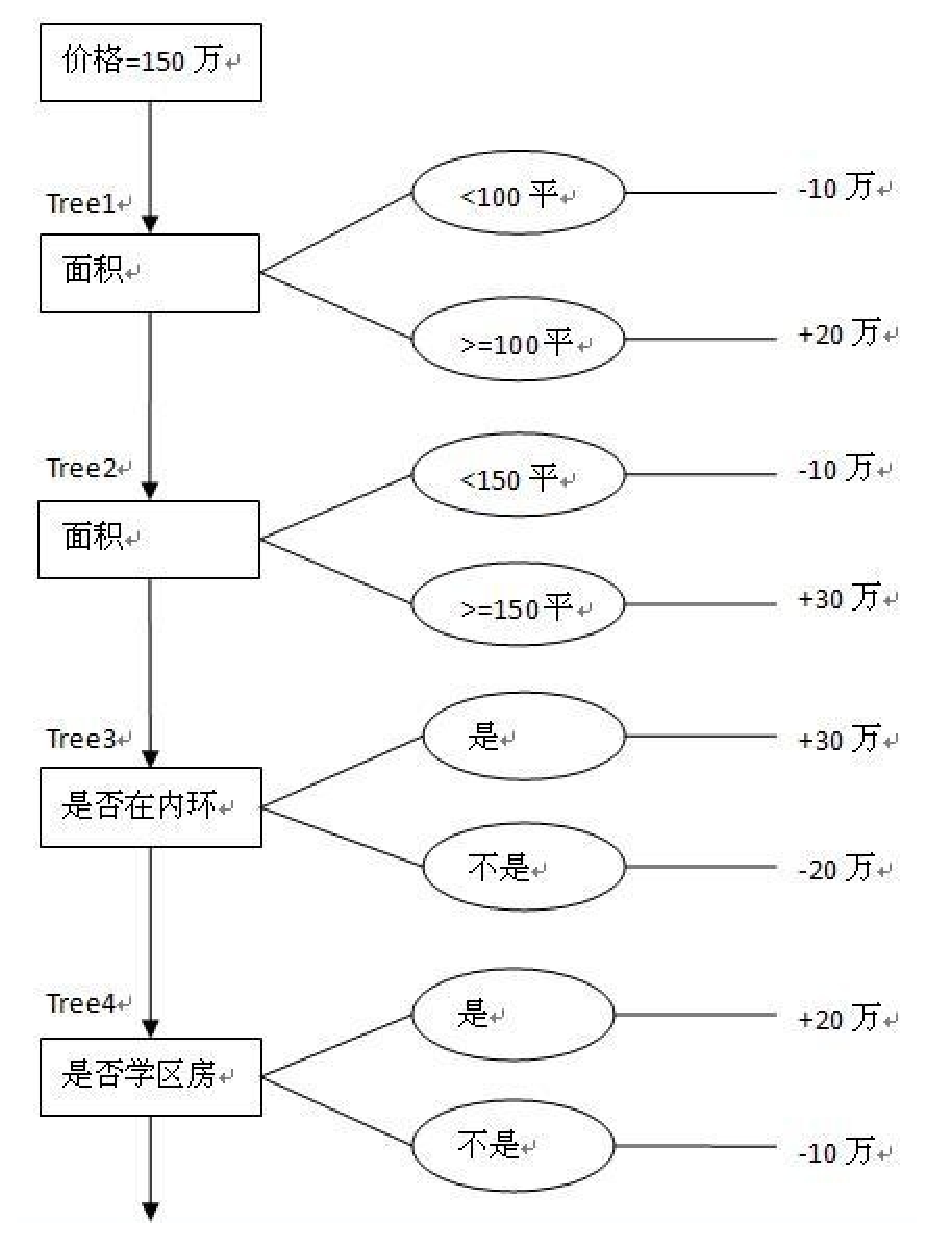
\includegraphics[width=0.85\textwidth,height=10cm]{figures/treelink.eps}
  \caption{商品房价格预测模型}\label{fig:treelink}
\end{figure}
对于新输入的样本,模型会赋予它一个初值(例子中初值设定为上海普通商品房价的均值150万),然后遍历每一棵决策树,每经过一棵树,都会对预测值进行调整修正,得到最后的预测结果:
\begin{equation}
    F(x) = F_0(x) + \sum\limits_{m=1}^M \beta_m h_m(x)
\end{equation}
比如,一个面积为120平米的内环非学区房,模型预测价格为:$150+20-10+30-10=180$万。
\end{example}

\subsection{排名问题}
\cite{busa2011ranking}和\cite{mohan2011web}使用逐点型排序学习方法,同序对型、序列型排序学习方法相比毫不逊色。\cite{busa2011ranking}在模型组合时引入序列型方法,取得不错的性能。\cite{mohan2011web}融合随机森林与GBDT的优点,使用随机森林模型初始化GBDT,不仅节省模型训练的时间,而且表现优于随机森林与GBDT算法。随机森林给了GBRT一个接近收敛的起始点,即使步长较小,也能很快结束迭代。

\chapter{聚类分析}
聚类分析是人类活动的一个重要内容,也是人类认知发展必然经历的一个过程。人类从孩童时期就在不断地完善潜意识下的分类模式,并逐渐掌握识别不同物理事物和抽象概念,如猫和狗、动物和植物、欢乐和痛苦等。所谓“物以类聚人以群分”,聚类是一个通过相似性关系划分抽象概念和物理对象的认知过程,有利于从复杂的信息结构中识别出规律性的数据分布特征,从而方便构建不同属性间的潜在关联。聚类分析是数据挖掘研究中一个非常活跃的研究课题,它不依赖人工标记数据揭示出数据内在关联与特征,已经成为机器学习、生物信息处理和市场分析等领域一个不可或缺的工具。

假设原始数据集$X=\{x_i\}_{i=1}^n$,$x_i\in \mathbb R^m$,聚类分析的目标是根据相似性关系将数据集划分至$K$个彼此不相交的子集(类簇或组),记作$\mathbb C=\{c_i\}_{i=1}^K$,则有
\[
    \bigcup\limits_{i=1}^K c_i = X,~~ c_s \cap c_t = \emptyset, \forall s\ne t = 1, 2,\ldots,K.
\]

\section{K-Means和K-Medoids}
K-Means算法从给定的K个初始簇心,根据数据点同簇心之间的距离,构造出K个簇类。一般地,K-Means算法是以迭代方式进行,在上一次构造的簇类上利用每个簇内所有数据点的均值选择新的簇心。K-Medoids算法与K-Means算法类似,不同之处在每次选取的质心,前者选中的必须是簇中的点。

\section{谱聚类}
传统聚类算法,如K-Means算法和K-Medoids算法,大多适用于凸球状样本空间,如果样本空间不是凸球状,则算法容易陷入局部最优。为了能够在任意形状的样本空间上做聚类分析,并使得聚类结果收敛于全局最优,研究人员设计出一种基于\textbf{谱图分割}(Spectral Graph Partition)的聚类算法:\textbf{谱聚类}(Spectral Clustering)。谱聚类算法以数据点为顶点,根据数据间的相似度连接数据顶点,构造一个无向加权图$G=(V, E)$,将聚类问题转化为谱图分割问题。在具体讨论谱聚类算法之前,我们先熟悉一下谱图分割算法及相关矩阵理论。

谱聚类算法计算出原始数据集$X$上的相似度矩阵(也称亲和矩阵)$A\in \mathbb R^{n\times n}$,根据一定的\textbf{连接规则}确定连接数据点的边,由此构造出含有$n$个顶点的无向加权图$G=(V, E)$,最终根据某种的\textbf{划分准则},可实现对$n$个数据顶点的聚类或分组。

谱聚类算法常用的连接规则有三种,对应地可以构造出三种不同的连接图:\textbf{全连接图}、\textbf{$\varepsilon-$近邻图}与\textbf{$K$近邻图},每一种连接图都对应一个边权矩阵$W\in \mathbb R^{n\times n}$。一般地,$W\ge 0$且$w_{ij}=0$表示节点$i$与$j$不相似,两个节点没有直接的连接通路。通常,数据相似度的选择依赖于数据空间的形状,比如凸球形的数据样本空间可以使用欧式距离定义相似性,对于非凸球形的样本空间最常见的是高斯核函数定义的相似性度量。
\begin{itemize}
  \item 如果直接使用数据相似度作为边的权值
        \[
            w_{ij}=a_{ij}, 1\le i,j \le n,
        \]
        我们可以构造出数据集$X$上的一个全连接图。
  \item 如果给定$\varepsilon>0$,并定义边的权值
        \[
            w_{ij}=\left\{
            \begin{array}{rl}
              a_{ij}, a_{ij}\ge \varepsilon,\\
              0, a_{ij}<\varepsilon,
            \end{array}
            \right.
        \]
        我们可以构造出数据集$X$上的一个$\varepsilon-$近邻图。
  \item 如果选定$K$值,连接各顶点的$K$个最近邻顶点,我们可以构造出$X$上的一个$K$近邻图。
\end{itemize}

我们下面从矩阵谱分析的角度分析谱聚类的理论基础,并在后续小节从图的划分角度分析它,建立谱聚类和矩阵论、谱图分割之间的紧密关系。
\subsection{谱分析}
假设$A\in \mathbb R^{n\times n}$是图$G$上顶点相似度矩阵,我们可以通过三种方法连接顶点,并构造对应图上边的权值矩阵$W\in \mathbb R^{n\times n}$。利用图上边的权值矩阵,我们可以计算各个顶点与其他顶点的连通度(Degree)。对于顶点$x_i$,其连通度定义为所有连接它和近邻顶点的边的权值之和,记作$d_i$,则有
\begin{equation}
    d_i = \sum\limits_{j=1}^n w_{ij},~~~D=\diag(d_1,\ldots,d_n)\in \mathbb R^{n\times n}.
\end{equation}
我们基于此构建三种类型的拉普拉斯矩阵(Graph Laplacian Matrix),它们是非标准化的拉普拉斯矩阵$L$、标准化对称的拉普拉斯矩阵$L_{\text{sym}}$和标准化随机游走的拉普拉斯矩阵$L_{\text{rw}}$:
\begin{eqnarray}
  L &=& D - W,\\
  L_\text{sym} &=& D^{-1/2} L D^{-1/2} = I - D^{-1/2} W D^{-1/2},\\
  L_\text{rw} &=& D^{-1} L = I - D^{-1} W.
\end{eqnarray}
由于拉普拉斯矩阵具有一些重要的基本性质,我们可以建立起矩阵谱系统和数据聚类的密切关联。
\begin{proposition}
非标准化拉普拉斯矩阵$L=D-W\in \mathbb R^{n\times n}$是对称的、半正定矩阵,对任意$f\in \mathbb R^n$都有
\[
    f^T L f = \frac{1}{2} \sum\limits_{1\le i,j\le n} w_{ij} (f_i-f_j)^2.
\]
它有$n$个非负实数特征值$\lambda_1\le \lambda_2 \le \cdots\le \lambda_n$,并且最小特征值$\lambda_1=0$,而其对应特征向量为$\mathbf 1$。
\end{proposition}

\begin{proposition}
假设$G$是一个无向图,边的权值非负,则矩阵$L$的零特征值的重数(Multiplicity)$K$与图$G$上独立连通子图的数目相同。如果记独立连通子图为$\{G_1,\ldots,G_K\}$,则零特征值对应的特征向量空间可由指标向量集$\{\mathbf 1_{G_1},\ldots,\mathbf 1_{G_K}\}$张成(Span)。
\end{proposition}
通过矩阵$L$的特征系统,利用其所有零特征值及对应特征向量可以直接将原始数据精确分组。一般地,原始数据存在大量的噪声干扰,非标准化的谱聚类算法计算拉普拉斯矩阵$L$ 的特征系统,固定或适应性地通过一个特征值阈值,选择出最小的$K$个特征值$\{\lambda_1,\ldots,\lambda_K\}$,利用对应特征向量$\{\alpha_1, \ldots, \alpha_K\}$ 将原始数据映射到一个低维空间
\[
    z_i = (\alpha_{1i}, \alpha_{2i}, \ldots, \alpha_{Ki})^T \in \mathbb R^K,~~~1\le i\le n
\]
在此低维数据集上运行K-Means聚类算法,对原始数据进行高效的近似分割。谱聚类算法存在一个明显的优势,它实际上不需显性的原始数据(维度不同或彼此异构),仅仅依赖于顶点之间的相似性关系,比其他聚类算法适用范围更广也更健壮。

\subsection{谱图分割}
目前,研究人员已经提出多种谱图分割方法,如最小割(Minimum Cut)、比率割(Ratio Cut)、标准割(Normalized Cut)等,将图的顶点分割成不相交的两个(Two-Way)或多个(K-Way)子图。我们将在后续章节逐一介绍它们。

假设图$G$可以被切割为$K$个彼此不相交的子图,分割准则是最小化被割边的权值之和,则有:
\begin{equation}\label{eq:mincut}
    \text{Cut}(c_1,\ldots, c_K) = \frac{1}{2} \sum\limits_{i=1}^K W(c_i,\bar c_i),
\end{equation}
其中,$\bar c_i$表示$c_i$的补集,$W(c_i,\bar c_i)$是$c_i$与$\bar c_i$间所有边的权值之和。由于最小割得到的子图分布可能极不均匀,出现部分子图为孤立点,其他子图所含数据点又太多。为此有人在最小割的基础上,提出改进的比率割:
\begin{equation}\label{eq:ratiocut}
    \text{RatioCut}(c_1,\ldots,c_K) = \frac{1}{2} \sum\limits_{i=1}^K \frac{W(c_i,\bar c_i)}{|c_i|} = \sum\limits_{i=1}^K \frac{\text{Cut}(c_i,\bar c_i)}{|c_i|},
\end{equation}
以及标准割:
\begin{equation}\label{eq:ratiocut}
    \text{NCut}(c_1,\ldots,c_K) = \frac{1}{2} \sum\limits_{i=1}^K \frac{W(c_i,\bar c_i)}{\text{vol}(c_i)} = \sum\limits_{i=1}^K \frac{\text{Cut}(c_i,\bar c_i)}{\text{vol}(c_i)},
\end{equation}
其中$|c|$表示$c$中所含顶点数目,$\text{vol}(c)=\sum\limits_{i\in c} d_i$表示$c$的容量。

\section{密度峰值聚类}
2014年,意大利国际高等研究院
\footnote{意大利国际高等研究院(\textit{it.} Scuola Internazionale Superiore di Studi Avanzati, \textit{en.} International School for Advanced Studies)创立于1978年,坐落于意大利北部城市里雅斯特(Trieste)。它是一所高级指导性学术研究中心,也是意大利第一所颁发博士学位的大学。它只在数学、物理及神经科学几个领域开展研究与教学,数学与神经科学在意大利排名第一,物理学排名第二,著名的国际理论物理中心就坐落在其校园内,声誉可与比萨高等师范学院(
\textit{it.} Scuola Normale Superiore di Pisa, \textit{en.} Advanced Normal School of Pisa)并肩。}
\href{http://people.sissa.it/~laio/index.html}{Alessandro Laio}教授的课题组提出一种基于密度峰值的高效聚类算法~\cite{rodriguez2014clustering},思想简明但效率和效果都很显著。它无需预先指定类簇数目,自动聚类时还能检测出异常点,一度成为年度聚类分析的热门话题。密度峰值聚类引入样本\textbf{局部密度}的概念,使得\textbf{每个类簇都是一个局部密度高地,而每个中心点都对应其类簇高地上的密度峰值,并为其近邻所环绕左右},故名\textbf{密度峰值聚类算法}。

\begin{figure}[ht]
  \centering
  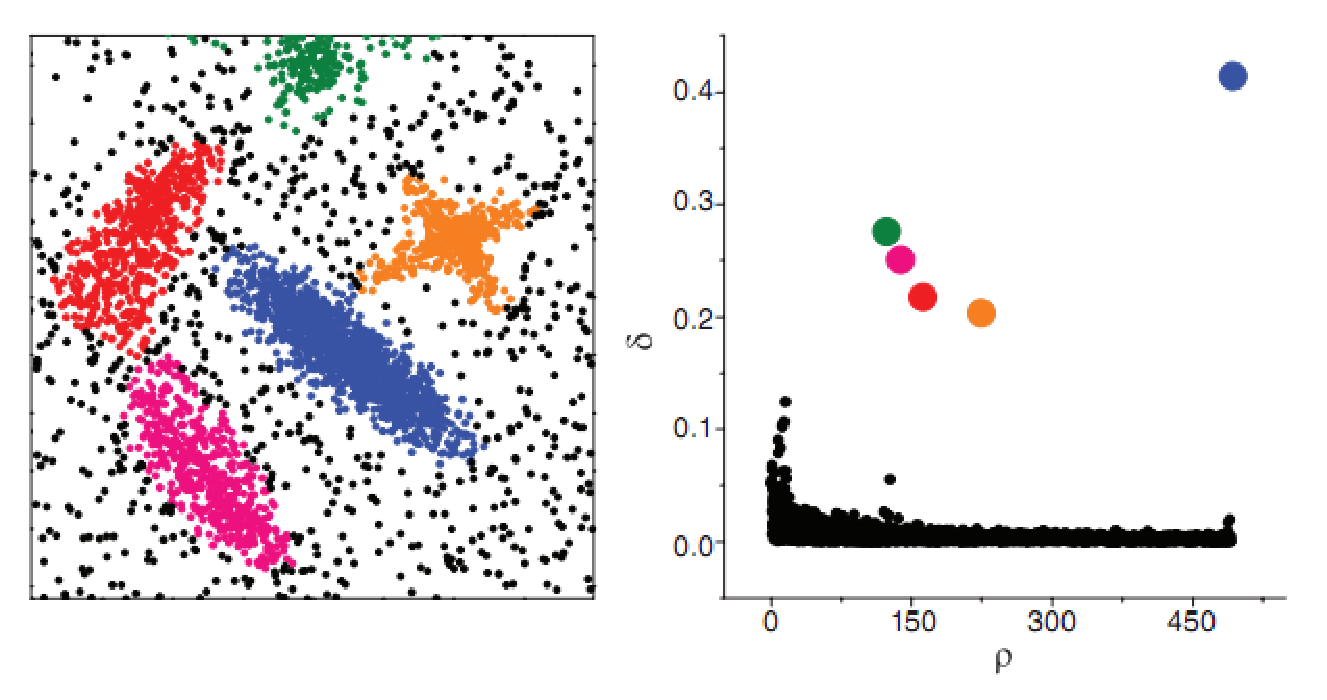
\includegraphics[width=0.8\textwidth, height=6cm]{figures/densitypeak_decisiongraph.eps}\\
  \caption{密度峰值聚类决策图~\cite{rodriguez2014clustering}}\label{fig:decisiongraph}
\end{figure}

密度峰值聚类算法依赖于两个指标:局部密度$\rho$、数据点与高密度近邻的最短距离$\delta$,后者依赖于前者以自动筛选类簇中心点。根据密度峰值聚类算法,数据点$x_i$ 的局部密度定义如下:
\begin{equation}\label{eq:localdensity}
    \rho_i = \sum\limits_{j=1}^n \chi(d_{ij}, d_c),~~~1\le i\le n,
\end{equation}
其中$d_c>0$是用户指定的截断距离,$d_{ij}$是$x_i$与$x_j$的空间距离,$\chi(\cdot)$是一个密度函数。一般地,距离$x_i$越近,对其密度的贡献越大,比如$\chi(d_{ij}, d_c) = e^{-d_{ij}/d_c}$。如果$\chi(d_{ij},d_c)=\ind(d_{ij} < d_c)$,则$x_i$的密度就是所有距离它在$d_c$范围内的近邻数目,计算密度时$d_c$范围外的点完全不予考虑。

密度峰值聚类算法将类簇内普通数据点视为其类簇中心点的随众,密度上低于中心点的局部密度,距离上相对其他高密度数据点中心数据点距离最近,每个类簇都是紧密围绕中心点而成的一个局部密度高地。一般地,聚类的显著特征是类簇内部紧密相联,而类簇之间则彼此分隔。
此外,算法还引入数据点与高密度近邻的最短距离
\begin{equation}
    \delta_i = \min\limits_{\rho_i < \rho_j} d_{ij},
\end{equation}
并对局部密度最大的数据点$\rho_i = \max\limits_{1\le j\le n} \rho_j$,定义其高密度最短距离
\begin{equation}
    \delta_i = \max\limits_{1\le j\le n} d_{ij}.
\end{equation}
如果以密度、高密度最短距离分别作横轴与纵轴,构建一个二维指标面板,则在面板右上角位置的点:密度高并且最短距离大,对应类簇的中心点。由此,指标面板可直接用作从数据集自动分离出类簇中心,实现自动分组的\textbf{决策图}(Decision Graph),如图\ref{fig:decisiongraph}。右侧决策图的右上角5个点对应五个类簇中心,其他点可依据各自高密度最近邻进行分组。从图\ref{fig:decisiongraph}和\ref{fig:dpcluster}可知密度峰值聚类算法性能优良、聚类准确。此外,密度峰值算法在分组时也存在一定的层次性,隐含不同类簇之间的蕴含关系,可以说它也是一个有效的\textbf{分层聚类方法}(Hierarchical Clustering Method)。
\begin{figure}[ht]
    \begin{minipage}[t]{\linewidth}
        \centering
          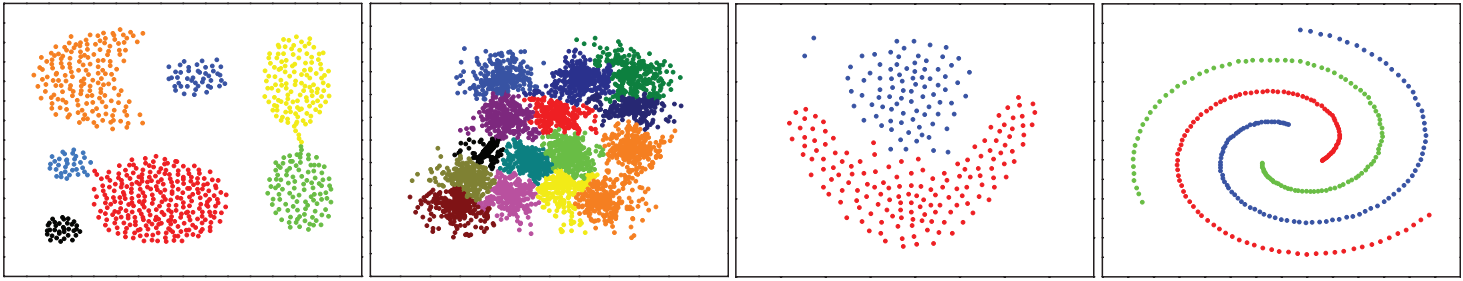
\includegraphics[width=0.95\textwidth,height=4cm]{figures/densitypeak_clustering}
    \end{minipage}
    \begin{minipage}[t]{\linewidth}
        \centering
          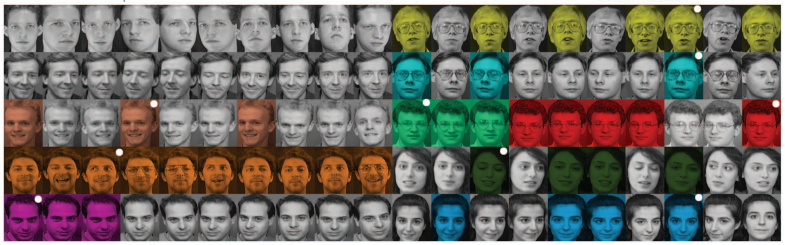
\includegraphics[width=0.95\textwidth,height=4cm]{figures/densitypeak_olivettiface}
    \end{minipage}
    \caption{经典人工数据集(上)与Olivetti人脸数据集(下)上密度峰值算法的性能~\cite{rodriguez2014clustering}}\label{fig:dpcluster}
\end{figure}

聚类算法在对不同数据分组时,可能存在可信度上的差异:有些可信度高,部分可信度差,后者很有可能就是异常点。为了能够从数据集中探测异常点,密度峰值聚类设法确定类簇间的模糊\textbf{边界}(Border),边界上的每个点与边界两侧的类簇中心的距离都在截断距离$d_c$ 范围之内。在确立类簇边界后,密度峰值聚类算法以边界上最高局部密度$\rho_c$作为检测异常点的阈值,当数据点的局部密度高于$\rho_c$,则认为此数据点的分组可信度高,称作\textbf{聚类核心
(Cluster Core)点},否则其可信度存疑,可以认定为\textbf{聚类光晕(Cluster Halo)点},即异常点。

\chapter{统计模型}
\section{EM算法}
EM(Expectation Maximization)算法是一种对缺失数据或者带有隐含变量的统计模型进行最大似然估计或最大后验估计的数值迭代算法\cite{dempster1977maximum}。本节简要介绍EM算法基本思想,并用它估计混合高斯模型的参数。

假设随机变量$X$的参数空间为$\theta$,则其的似然函数可表示为$P(X; \theta)$,根据最大似然估计法,我们可以通过最大化$P(X|\theta)$解出参数的似然估计值,等价地可以最大化其对数值:
\begin{equation}
  \max\limits_{\theta\in \Theta} L(\theta) = \log P(X; \theta).
\end{equation}
EM算法通过迭代的方式最大化对数似然函数,设当前参数估计值为$\theta_n$,则最大化对数似然函数即等价于解下面形式的目标函数:
\begin{equation}
  \max\limits_{\theta\in \Theta} L(\theta) - L(\theta_n) = \log P(X; \theta) - \log P(X; \theta_n).
\end{equation}
引入隐含变量$Z$,利用全概率公式$P(X; \theta) = \sum\limits_z P(X| z;\theta)P(z;\theta)$展开$L(\theta) - L(\theta_n)$,则有等式
\begin{equation}
\begin{array}{lcl}
  L(\theta) - L(\theta_n)  & = & \log\sum\limits_z P(X| z;\theta)P(z;\theta) - \log P(X;\theta_n) \\
  & = & \log\sum\limits_z P(X|z;\theta)P(z;\theta) \frac{P(z| X;\theta_n)}{P(z| X;\theta_n)} - \log P(X; \theta_n),
\end{array}
\end{equation}
由$\sum\limits_z P(z| X;\theta_n) = 1$与对数函数的凸性可知
\begin{eqnarray}
  L(\theta) - L(\theta_n) & \ge & \sum\limits_z P(z| X;\theta_n) \log \frac{P(X| z;\theta)P(z;\theta)}{P(z| X;\theta_n)} - \log P(X; \theta_n)\\
  & = & \sum\limits_z P(z| X;\theta_n) \log \frac{P(X|z;\theta)P(z;\theta)}{P(z| X;\theta_n)P(X;\theta_n)}\\
  & \triangleq & Q(\theta, \theta_n) - U(\theta_n)
\end{eqnarray}
其中,
\begin{eqnarray}
  &&Q(\theta, \theta_n) =  \sum\limits_z P(z|X;\theta_n) \log \big[P(X|z; \theta)P(z;\theta)\big],\\
  &&U(\theta_n) = \sum\limits_z P(z|X;\theta_n) \log \big[P(z|X; \theta_n)P(X;\theta_n)\big].
\end{eqnarray}
最大化$L(\theta)$可以通过其最大化$L(\theta) - L(\theta_n)$的一个下界近似趋近。既然$U(\theta_n)$与$\theta$完全无关,则等价于最大化$Q(\theta, \theta_n)$
\begin{equation}
    \max\limits_{\theta\in \Theta} \sum\limits_z P(z|X;\theta_n) \log P(X,z; \theta) = \sum\limits_z E_{z|X;\theta_n} \log P(X,z; \theta).
\end{equation}
至此,我们导出EM算法每次迭代所经历的两个基本步骤:
\begin{itemize}
  \item \textbf{E步骤}:$E_{z|X;\theta_n} \log P(X,z;\theta)$
  \item \textbf{M步骤}:$\max\limits_{\theta\in \Theta} E_{z|X;\theta_n} \log P(X,z;\theta)$
\end{itemize}

\subsection{高斯混合模型}
\textbf{高斯混合模型}(Gaussian Mixture Model,GMM),顾名思义是多个高斯模型的混合。假设混合模型$\Lambda$每个成员都是一个高斯模型,给定数据集$X=\{x_1, x_2,\ldots, x_n\}$,我们可以使用最大似然估计法估计模型的参数。假设数据集$X$所有样本独立同分布,可以构建对数似然函数
\begin{equation}
    L(X; \Lambda) = \sum\limits_i \log p(x_i; \Lambda),
\end{equation}
其中,$x_i\in \mathbb R^d, i = 1, 2, \ldots, n$。

混合模型是一个黑盒,我们的目标是剖解其结构,并利用EM算法估计各个成员参数。现在引入隐含随机变量$Z$,并根据全概率公式
\begin{equation}\label{eq:totalprob}
    p(x_i; \Lambda, p(z), z\in \mathbb Z) = \sum\limits_z p(z) p(x_i|z; \Lambda)
\end{equation}
改写对数似然函数
\begin{equation}
    L(X; \theta) = \sum\limits_i \log p(x_i; \theta) = \sum\limits_i \log \Big[\sum\limits_z p(z) p(x_i|z; \Lambda)\Big].
\end{equation}
其中,
\[\Lambda = \{\mu_z, \Sigma_z, z\in \mathbb Z\}, ~~\mu_z \in \mathbb R^d, \Sigma_z\in \mathbb R^{d\times d}\]
是混合模型中各个成员的均值向量与协方差矩阵,并且依赖于隐含随机变量$Z$,成员数目对应$\mathbb Z$的容量。新引入的概率分布$p(z),z\in \mathbb Z$表示各个成员在混合模型中的权重,且满足具有下面两个基本性质:
\begin{equation}
    0 < p(z) < 1,~~\sum\limits_z p(z) = 1.
\end{equation}
参数$\theta$对参数$\Lambda$与$p(z), z\in \mathbb Z$的组合定义:
\[\theta = \{\mu_z, \Sigma_z, p(z), z\in \mathbb Z\}.\]
根据混合模型的定义可知$x|z;\Lambda \sim N(\mu_z, \Sigma_z)$,则随机变量$x|z;\Lambda$对应的概率密度函数为
\begin{equation}
    p(x|z;\Lambda) = \frac{1}{(2\pi)^{d/2} |\Sigma_z|^{1/2}} \exp \Big\{-\frac{1}{2} (x-\mu_z)^T \Sigma_z^{-1} (x-\mu_z)\Big\}.
\end{equation}
假设混合模型的最大似然估计为$\hat \theta_{MLE}$,则有
\begin{equation}
    \hat \theta_{MLE} = \argmax\limits_{\theta\in \Theta} L(X; \theta) = \argmax\limits_{\theta\in \Theta} \sum\limits_i \log \Big[\sum\limits_z p(z) p(x_i|z; \Lambda)\Big].
\end{equation}

我们下面利用已知约束条件
\[
   0 < p(z) < 1,~~\sum\limits_z p(z) = 1,
\]
确定对数似然函数极值所对应的最优参数$\hat \Lambda$和$\hat p(z), z\in \mathbb Z$。由于约束条件只与参数$p(z)$相关,而参数$\Lambda$又不依赖于$p(z)$,故此可直接通过对数似然函数关于参数$\Lambda$的偏导解出对应的$\hat \Lambda$。当然,确定最优的$p(z)$,则相对复杂一些,要通过拉格朗日乘子法搜索。

我们现在利用拉格朗日乘子法搜索最优的$p(z), z \in \mathbb Z$:引入拉格朗日乘子$\lambda > 0$,构造拉格朗日函数
\begin{equation}
    \mathscr L = L(X; \theta) - \lambda (\sum\limits_z p(z) - 1).
\end{equation}
然后求关于$\lambda$与$p(z)$的偏导,并令它们为零,可以得到方程组
\begin{equation}\label{eq:partialarray}
    \left\{
        \begin{array}{lcl}
            \partial \mathscr L/\partial \lambda &=& 1 - \sum\limits_z p(z) = 0,\\
            \partial \mathscr L/\partial p(z) &=& \frac{\partial L(X; \theta)}{\partial p(z)} - \lambda = 0, ~~z\in \mathbb Z.
        \end{array}
    \right.
\end{equation}
在具体展开对数似然函数关于$p(z)$的偏导之前,可以看出:
\begin{equation}\label{eq:partialtheta}
    \frac{\partial L(X; \theta)}{\partial \theta} = \sum\limits_i \frac{1}{p(x_i; \theta)} \frac{p(x_i; \theta)}{\partial \theta},
\end{equation}
再根据全概率公式
\[p(x_i; \theta) = \sum\limits_z p(z) p(x_i|z; \Lambda),\]
我们可以推导$p(x_i; \theta)$关于$p(z)$的偏导:
\begin{equation}
    \frac{p(x_i; \theta)}{\partial p(z)} = p(x_i|z; \Lambda),
\end{equation}
将其代入式子\eqref{eq:partialtheta}可知
\[
\frac{\partial L(X; \theta)}{\partial p(z)} = \sum\limits_i \frac{p(x_i|z; \Lambda)}{p(x_i; \theta)}
    = \sum\limits_i \frac{p(x_i|z; \Lambda) p(z)}{p(x_i; \theta)} \frac{1}{p(z)}
    = \frac{1}{p(z)} \sum\limits_i p(z|x_i; \Lambda),
\]
再将其代入方程组\eqref{eq:partialarray},可以推得
\begin{equation}\label{eq:optimalpz}
    \hat p(z) = \frac{\sum\limits_i p(z|x_i;\Lambda)}{\sum\limits_z\sum\limits_i p(z|x_i;\Lambda)}
    = \frac{\sum\limits_i p(z|x_i;\Lambda)}{\sum\limits_i \sum\limits_z p(z|x_i;\Lambda)}
    = \frac{1}{n} \sum\limits_i p(z|x_i;\Lambda).
\end{equation}

我们继续从式子\eqref{eq:partialtheta}和全概率公式\eqref{eq:totalprob}出发,推导$p(x_i; \Lambda)$关于$\Lambda$的偏导:
\begin{equation}\label{eq:partiallambda}
    \frac{\partial L(X; \theta)}{\partial \Lambda}% = \sum\limits_i \frac{1}{p(x_i; \theta)} \frac{\partial p(x_i; \theta)}{\partial \Lambda}
   % = \sum\limits_i \frac{p(z)}{p(x_i; \theta)} \frac{\partial p(x_i|z;\Lambda)}{\partial \Lambda}
    = \sum\limits_i \frac{p(z) p(x_i|z;\Lambda)}{p(x_i; \theta)} \frac{\partial \log p(x_i|z;\Lambda)}{\partial \Lambda}
    = \sum\limits_i p(z|x_i;\Lambda) \frac{\partial \log p(x_i|z;\Lambda)}{\partial \Lambda}.
\end{equation}

根据变量$x_i|z;\Lambda$的概率密度函数,及其对数形式
\[
  \log p(x_i|z;\Lambda) = - \frac{d}{2} \log (2\pi) - \frac{1}{2} \log |\Sigma_z| - \frac{1}{2} (x_i - \mu_z)^T \Sigma_z^{-1} (x_i - \mu_z),
\]
其中协方差矩阵$\Sigma_z$是非奇异对称实矩阵,我们可以推导出$\log p(x_i|z;\Lambda)$关于均值向量$\mu_z$和协方差矩阵$\Sigma_z$的偏导函数:
\[
    \frac{\partial \log p(x_i|z;\Lambda)}{\partial \mu_z} %= \frac{1}{2} \Big[\Sigma_z^{-1} + \big(\Sigma_z^{-1}\big)^T\Big](x_i - \mu_z)
    = \Sigma_z^{-1} (x_i - \mu_z)
\]
将其代入等式\eqref{eq:partiallambda},再根据极值条件有:
\[
    \frac{\partial L(X; \theta)}{\partial \mu_z} = \sum\limits_i p(z|x_i;\Lambda) \Sigma_z^{-1} (x_i - \mu_z)
    = \Sigma_z^{-1} \sum\limits_i p(z|x_i;\Lambda) (x_i - \mu_z)
    = 0,
\]
从而解出最优解
\begin{equation}\label{optimalmuz}
    \hat \mu_z = \frac{\sum\limits_i p(z|x_i;\Lambda) x_i}{\sum\limits_i p(z|x_i;\Lambda)}.
\end{equation}

下面我们继续推导$\log p(x_i|z;\Lambda)$关于协方差矩阵$\Sigma_z$的偏导函数:
\begin{equation}\label{eq:partialsigmaz}
    \frac{\partial \log p(x_i|z;\Lambda)}{\partial \Sigma_z} = -\frac{1}{2} \Big[\frac{\partial \log |\Sigma_z|}{\partial \Sigma_z} + \frac{\partial (x_i - \mu_z)^T \Sigma_z^{-1} (x_i - \mu_z)}{\partial \Sigma_z}\Big]
    \triangleq -\frac{1}{2}\big[V_1(\Sigma_z) + V_2(\Sigma_z)\big]
\end{equation}
等式右侧第一部分$V_1(\Sigma_z)\in \mathbb R$是关于可逆矩阵的行列式求导,第二部分$V_2(\Sigma_z)\in \mathbb R$则涉及到矩阵迹的求导。在具体展开之前,我们先来看看矩阵求导的相关性质:
\begin{eqnarray}
  &&\frac{\partial \log |A|}{\partial A} = \big(A^{-1}\big)^T,~~|A|>0 \\
  &&\tr(ABC) = \tr(BCA) = \tr(CAB), ~~ABC\in \mathbb R \\
  &&\frac{\partial A^{-1} B}{\partial A} = -\big(A^{-1}\big)^T B \big(A^{-1}\big)^T, ~~|A|>0
\end{eqnarray}
利用这些性质,我们可以求$V_1(\Sigma_z)$与$V_2(\Sigma_z)$关于$\Sigma_z$的偏导函数:
\begin{eqnarray}
    \frac{\partial V_1(\Sigma_z)}{\partial \Sigma_z} &=& \big(\Sigma_z^{-1}\big)^T\\
    \frac{\partial V_2(\Sigma_z)}{\partial \Sigma_z} &=& \frac{\partial \tr\Big(\Sigma_z^{-1} (x_i - \mu_z)(x_i - \mu_z)^T\Big)}{\partial \Sigma_z}\\
    &=& -\big(\Sigma_z^{-1}\big)^T (x_i - \mu_z)(x_i - \mu_z)^T \big(\Sigma_z^{-1}\big)^T
\end{eqnarray}
同时代入式子\eqref{eq:partialsigmaz}与\eqref{eq:partiallambda},再根据极值条件有:
\[
    \frac{\partial L(X; \theta)}{\partial \Sigma_z} = -\frac{1}{2} \sum\limits_i p(z|x_i;\Lambda) \Big[\big(\Sigma_z^{-1}\big)^T -\big(\Sigma_z^{-1}\big)^T (x_i - \mu_z)(x_i - \mu_z)^T \big(\Sigma_z^{-1}\big)^T \Big]
    =0,
\]
从而解出最优解
\begin{equation}\label{optimalsigmaz}
    \hat \Sigma_z = \frac{\sum\limits_i p(z|x_i;\Lambda) (x_i - \mu_z)(x_i - \mu_z)^T }{\sum\limits_i p(z|x_i;\Lambda)}.
\end{equation}
综上可知最优解
\begin{eqnarray}
  &&\hat p(z) =  \frac{1}{n} \sum\limits_i \textcolor{red}{p(z|x_i;\Lambda)}\\
  &&\hat \mu_z = \frac{\sum\limits_i \textcolor{red}{p(z|x_i;\Lambda)} x_i}{\sum\limits_i p(z|x_i;\Lambda)}\\
  &&\hat \Sigma_z = \frac{\sum\limits_i \textcolor{red}{p(z|x_i;\Lambda)} (x_i - \mu_z)(x_i - \mu_z)^T }{\sum\limits_i p(z|x_i;\Lambda)}
\end{eqnarray}
都与$\textcolor{red}{p(z|x_i;\Lambda)}$紧密相关,而根据贝叶斯定理又有
\[
    p(z|x_i;\Lambda) = \frac{p(z)p(x_i|z;\Lambda)}{p(x_i;\theta)} = \frac{p(z)p(x_i|z;\Lambda)}{\sum\limits_z p(z) p(x_i|z;\Lambda)},
\]
其中
\[
    p(x_i|z;\Lambda) = \frac{1}{(2\pi)^{d/2} |\Sigma_z|^{1/2}} \exp \Big\{-\frac{1}{2} (x_i-\mu_z)^T \Sigma_z^{-1} (x_i-\mu_z)\Big\},
\]
可见参数最优解又决定了$\textcolor{red}{p(z|x_i;\Lambda)}$,彼此相互依赖。EM算法通过循环交替地使用E步骤与M步骤算出最优解。

EM算法引入的隐含随机变量在不同应用情景下具有不同的含义,比如聚类分析问题中的类别属性、词性分析问题中的单词词性等。
\section{概率隐语义分析}%Probabilistic Latent Semantic Analysis: pLSA
\section{隐含狄利克雷分布}%Latent Dirichlet Allocation: LDA

\section{最大熵模型}
最大熵模型(Maximum Entropy Model, MaxEnt)与隐马尔科夫模型(Hidden Markov Model, HMM)\cite{jurafsky1999speech}是自然语言处理(如词性标注、中文分词、句子边界识别、浅层句法分析及文本分类等\cite{berger1996maximum})和语音识别问题中得到广泛应用的两种统计模型。本节主要介绍最大熵模型,下一节重点介绍隐马尔科夫模型。

\subsection{最大熵原理}
1957年,物理学家Edwin Thompson Jaynes\cite{jaynes1957information1,jaynes1957information2}最早阐述了\textbf{最大熵原理}:
\begin{quote}
  \textit{Information theory provides a constructive criterion for setting up probability distributions on the basis of partial knowledge, and leads to a type of statistical inference which is called the maximum entropy estimate. It is least biased estimate possible on the given information; i.e., it is maximally noncommittal with regard to missing information.}
\end{quote}

最大熵原理是概率模型学习的一个准则,它对未知事物不做任何主观假设,在预测一个随机事件的概率分布时,在满足所有已知约束条件下,对未知情况不含任何主观偏见的结果是满足均匀概率分布,此时概率分布的信息熵做大,预测的风险也最小。根据最大熵原理推导的模型称作“最大熵模型”,比如投资学中“不要把所有的鸡蛋都放在一个篮子里”就是一种典型的最大熵策略:当出现不确定性时,就要保留各种可能性。

最大熵模型在形式上是最漂亮的统计模型,在实现上却是最复杂的模型之一,至今天为止,世界上能有效实现快速算法的人寥寥无几。第一个解决最大熵模型的优化算法是1972年John Darroch和Douglas Ratcliff联合提出的广义迭代尺度算法(Generalized Iterative Scaling, GIS)\cite{darroch1972generalized}。1989年,匈牙利著名数学家、信息论最高奖香农奖得主Imre Csiszar 从几何学角度详细分析最大熵模型\cite{csiszar1989geometric},并证明“对任何一组相容的信息,最大熵模型不仅存在,并且以指数函数的形式唯一存在”。由于GIS迭代算法效率低、复杂度高、稳定性差,在实际应用中鲜有人使用它。1997年,Della Pietra等人提出一种改进的迭代尺度算法IIS (Improved Iterative Scaling)\cite{della1997inducing},将最大熵模型训练所需时间降低了一两个数量级,成为当前最常用的最大熵模型优化算法。后来,Della Pietra兄弟二人离开IBM,退出学术圈转战金融界大显身手,加入当时籍籍无名的文艺复兴技术公司(Renaissance Technologies)。文艺复兴公司是数学家James Simons于1982年创立,已经发展为当今世界最成功的一家对冲基金公司。在金融市场,决定股票价格的因素成千上万,而最大熵方法正是建立能够同时满足所有不同条件的模型,文艺复兴技术公司的科学家们(包括Della Pietra兄弟)使用最大熵方法和其他先进的数学工具,建立量化的股票价格预测模型,获得巨大的成功。从1982年基金创立至今资产规模已经达到三百多亿美元,其净回报率高达平均每年34\%,远超股神巴菲特的旗舰公司——伯克希尔$\cdot$哈撒韦公司(Berkshire Hathaway)\cite{wu2012math}。

信息论提供了一种基于部分知识建立概率分布的构造性准则,由此而产生了一类统计推断(Statistical Inference)方法\footnote{统计推断方法是根据带随机性的观测数据(样本)以及问题的条件和假定(模型),而对未知事物作出的,以概率形式表述的推断。它是数理统计学的主要任务,其理论和方法构成数理统计学的主要内容。},即最大熵估计。在基于给定信息进行估计的所有方法中,最大熵估计属于最无偏见的一种,它对缺失的信息保留了最大的灵活性和不确定性\cite{jaynes1957information}。

根据最大熵原理,概率模型必须满足所有由已知事实构成的约束条件,并且在没有更多信息的条件下,其他不确定或未知的事件都是“等可能地发生”,而等可能的概率模型对应的熵最大。我们下面使用一个简单的实例介绍最大熵原理。
\begin{example}
假设随机投掷骰子,出现的点数$X$,则其可能取值为$\{1,2,\ldots,6\}$。对于某次投掷实验,估计各个点数出现的概率$P(X=1), P(X=2), \ldots, P(X=6)$。如果没有任何其他关于骰子的信息,根据最大熵对其点数出现的概率分布进行估计,则各个点数出现的概率相等$P(X=i)=1/6, i = 1, 2, \ldots, 6$。如果我们知道投掷骰子出现点数$1$和$6$的概率之和等于1/2,即概率分布的约束条件有两个:
\[P(X=1) + P(X=6) = 1/2, P(X=2) + P(X=3) + P(X=4) + P(X=5) = 1/2.\]
满足两个约束条件的概率分布有无穷多个,根据最大熵原理,可以认为出现点数1和点数6的概率是相等的,出现其他点数彼此也是等概率事件,即
\[P(X=1) = P(X=6) = 1/4, P(X=2) = P(X=3) = P(X=4) = P(X=5) = 1/8.\]
\end{example}

\subsection{最大熵模型}
假设分类模型是一个条件概率分布$P(Y|X)$,给定训练数据集$\{(x_1, y_1),(x_2,y_2),\ldots, (x_N, y_N)\}$,我们学习的目标是根据最大熵原理选择最佳的分类模型。从训练数据集,我们可以确定联合概率分布$P(X,Y)$的经验概率分布$\tilde{P}(X,Y)$、边际概率分布$P(X)$的经验概率分布$\tilde{P}(X)$,则有
\[\tilde{P}(x,y) = \frac{1}{N}C(x, y)\]
\[\tilde{P}(x) = \frac{1}{N}C(x)\]
其中,$C(x, y)$表示训练数据集中样本$(x,y)$出现的频数,$C(x)$ 表示训练数据集中输入$x$出现的频数。$N$表示训练样本容量。

为刻画已知事实,最大熵模型定义输入$x$与输出$y$的二值特征函数$f(x,y)$:当输入$x$与输出$y$之间存在某一事实关系,则$f(x,y)$ 取值1,否则取值0,其数学定义为
\[f(x,y) = \left\{
\begin{array}{ll}
    1, & x\text{与}y\text{存在某一事实},\\
    0, & \text{否则}.
\end{array}
\right.\]
如果给定训练数据集,则特征函数$f(x,y)$在训练集上的期望值$E_{\tilde P}(f)$定义如下:
\[E_{\tilde P}(f)=\sum \limits_{x,y} \tilde P(x,y) f(x,y)\]
其中,$\tilde P(x,y)$是样本$(x,y)$在数据集中的经验分布,可根据样本$(x,y)$在训练集上的频数进行计算。如果我们能够从数据集训练得到概率模型$P(y|x)$,则特征函数关于此概率模型的期望$E_P(f)$可写作:
\[E_P(f) = \sum\limits_{x,y} P(x, y) f(x,y) = \sum\limits_{x,y} \textcolor{red}{P(x)} P(y|x) f(x,y) = \sum\limits_{x,y} \textcolor{red}{\tilde P(x)} P(y|x) f(x,y)\]
其中,$\tilde P(x)$是样本输入$x$在数据集中的经验分布,与$\tilde P(x,y)$类似,可以从训练集中统计出相应频数并计算得到。我们对于输入真实的先验分布$P(x)$并不关心,从而直接使用数据集上的经验分布$\tilde P(x)$代替。如果概率模型能够充分刻画训练数据的所有信息,则可以认为特征函数的两种期望相等,即有
\begin{equation}
    E_P(f) = E_{\tilde{P}}(f).
\end{equation}
假设存在$n$个特征函数$f_i(x,y),i=1,2,\ldots,n$,刻画输入$x$与输出$y$的$n$种事实关系,它们就构成$n$个约束条件。

\begin{definition}[最大熵模型]
假设满足所有约束条件的概率模型集合为
\begin{equation}
   \mathcal P = \{P| E_P(f_i) = E_{\tilde{P}}(f_i), i = 1,2,\ldots,n\},
\end{equation}
则模型集合中条件熵
\begin{equation}
    H(P) = \sum\limits_x \textcolor{red}{P(x)} \Big(-\sum\limits_y P(y|x) \log P(y|x)\Big) = -\sum\limits_{x,y} \textcolor{red}{\tilde{P}(x)} P(y|x) \log P(y|x),
\end{equation}
最大的模型称作\textbf{最大熵模型}。
\end{definition}

\noindent 最大熵模型是如下带约束最优化问题
\begin{equation}\label{eq:maxent}
  \begin{array}{ll}
    \textit{max} & H(P) = -\sum\limits_{x,y} \tilde{P}(x)P(y|x) \log P(y|x)\\
    \textit{s.t.}& E_P(f_i) = E_{\tilde{P}}(f_i), i = 1,2,\ldots,n, \\
    & \sum\limits_y P(y|x) = 1,
  \end{array}
\end{equation}
的解,它等价于如下形式的最小化问题:
\begin{equation}
  \begin{array}{ll}
    \textit{min} & -H(P) = \sum\limits_{x,y} \tilde{P}(x)P(y|x) \log P(y|x)\\
    \textit{s.t.}&  E_{\tilde{P}}(f_i) - E_P(f_i)= 0, i = 1,2,\ldots,n, \\
    & \sum\limits_y P(y|x) = 1.
  \end{array}
\end{equation}
我们引入拉格朗日乘子$\lambda_0,\lambda_1,\lambda_2,\ldots, \lambda_n$,定义拉格朗日函数$L(P,\lambda)$:
\begin{equation}
    L(P,\lambda) = -H(P) + \lambda_0 \big(1-\sum\limits_{y} P(y|x)\big) + \sum\limits_i \lambda_i\big(E_{\tilde{P}}(f_i) - E_P(f_i)\big),
\end{equation}
将其转化为无约束最优化问题。
由于函数$L(P,\lambda)$是$P$的凸函数,原始问题$\min\limits_{P\in \mathcal P} \max\limits_{\lambda} L(P,\lambda)$与对偶问题$\max\limits_{\lambda} \min\limits_{P\in \mathcal P} L(P,\lambda)$的解等价,我们通过解对偶问题可以得到原始问题的解。对拉格朗日函数求关于$P(y|x)$ 的偏导,并令其为0,则有
\begin{equation}
    \frac{\partial L(P,\lambda)}{\partial P(y|x)} = \tilde{P}(x)\big[1 + \log P(y|x)\big] - \lambda_0 - \tilde{P}(x) \sum\limits_i \lambda_i f_i(x,y) = 0,
\end{equation}
由于$\tilde{P}(x)>0$,两边同除以$\tilde{P}(x)$,经过整理可得:
\begin{equation}
    P(y|x) = \exp\Big(\sum\limits_i \lambda_i f_i(x,y) + \frac{\lambda_0}{\tilde{P}(x)} - 1\Big),
\end{equation}
根据$\sum\limits_y P(y|x)=1$,可对其归一化处理,可得最大熵模型:
\begin{equation}
    P_\lambda(y|x) = \exp\Big(\sum\limits_i \lambda_i f_i(x,y)\Big)\frac{1}{Z_\lambda(x)},
\end{equation}
其中,$Z_\lambda(x)$是归一化因子:
\begin{equation}
    Z_\lambda(x) = \sum\limits_y \exp\Big(\sum\limits_i \lambda_i f_i(x,y)\Big).
\end{equation}
根据对偶理论,将最优概率模型$P_\lambda(y|x)$带入拉格朗日函数,最大化目标函数
\begin{equation}\label{eq:dualmaximum}
    \begin{array}{lcl}
        L(\lambda) & = &\sum\limits_{x,y} \tilde{P}(x) P_\lambda(y|x) \log P_\lambda(y|x) + \sum\limits_i \lambda_i \sum\limits_{x,y} \Big(\tilde P(x,y)-\tilde{P}(x) P_\lambda(y|x) \Big) f_i(x,y)\\
        & = & \sum\limits_{x,y} \tilde P(x,y) \sum\limits_i \lambda_i f_i(x,y) -\sum\limits_x \tilde P(x) \log Z_\lambda(x),
    \end{array}
\end{equation}
以确定最优模型参数$\lambda^*$。由于函数$L(\lambda)$是光滑凸函数,大多数优化算法,如梯度下降法、牛顿法、拟牛顿法、改进的迭代尺度(Improved Iterative Scaling, IIS)算法均适用,并搜索到$L(\lambda)$的全局最优解。我们下面介绍基于改进的迭代尺度算法搜索最大熵模型参数。

\subsection{参数优化 - IIS算法}
IIS算法通过迭代的方法搜索最优模型参数,假设当前参数向量为$\lambda=(\lambda_1,\lambda_2,\ldots,\lambda_n)^T$,只要在下次迭代时搜索到一个新的参数向量$\lambda+\delta=(\lambda_1+\delta_1, \lambda_2+\delta_2,\ldots, \lambda_n+\delta_n)^T$,使得目标函数$L(\lambda)$增大,依此不断更新参数,最终可以确定最优参数向量。当参数从$\lambda$更新至$\lambda+\delta$,目标函数$L(\lambda)$的变化量$\Delta L(\delta|\lambda) = L(\lambda+\delta) - L(\lambda)$:
\begin{equation}
    \begin{array}{lcl}
         \Delta L(\delta|\lambda) &=& \sum\limits_{x,y} \tilde P(x,y) \sum\limits_i \delta_i f_i(x,y)-\sum\limits_x \tilde P(x) \Big(\log Z_{\lambda+\delta}(x) - \log Z_\lambda(x) \Big)\\
        &=& \sum\limits_{x,y} \tilde P(x,y) \sum\limits_i \delta_i f_i(x,y)-\sum\limits_x \tilde P(x) \log \frac{Z_{\lambda+\delta}(x)}{Z_\lambda(x)}.
    \end{array}
\end{equation}
根据不等式$-\log \alpha \ge 1 - \alpha, \alpha > 0$,则有
\begin{equation}
    \begin{array}{lcl}
    \Delta L(\delta|\lambda) &\ge& \sum\limits_{x,y} \tilde P(x,y) \sum\limits_i \delta_i f_i(x,y)+\sum\limits_x \tilde P(x) (1-\frac{Z_{\lambda+\delta}(x)}{Z_\lambda(x)})\\
    & = & \sum\limits_{x,y} \tilde P(x,y) \sum\limits_i \delta_i f_i(x,y) + 1 - \sum\limits_x \tilde P(x) \sum\limits_y P_\lambda(y|x) \exp\Big(\sum\limits_i \delta_i f_i(x,y)\Big)\\
    & \triangleq & A(\delta|\lambda),
    \end{array}
\end{equation}
并确定目标函数变化量的一个下界$A(\delta|\lambda)$。如果我们可以搜索到一条使下界增加的路径,则目标函数$\Delta L(\delta|\lambda)$循此路径自然也会增加。由于$A(\delta|\lambda)$表达式中含有参数$\delta_i$的加和指数项,彼此相互依赖,不易同步更新所有维度的参数。我们改写下界函数$A(\delta|\lambda)$
\begin{equation}
    A(\delta|\lambda) = \sum\limits_{x,y} \tilde P(x,y) \sum\limits_i \delta_i f_i(x,y) + 1 - \sum\limits_x \tilde P(x) \sum\limits_y P_\lambda(y|x) \exp\Big(g(x,y) \sum\limits_i \frac{\delta_i f_i(x,y)}{g(x,y)}\Big),
\end{equation}
其中,
\[g(x,y) = \sum\limits_i f_i(x,y).\]
由于\[0\le \frac{f_i(x,y)}{g(x,y)} \le 1, \sum\limits_i \frac{f_i(x,y)}{g(x,y)} = 1,\]
根据Jensen不等式
\begin{equation}
    \exp\Big(\sum\limits_i \frac{f_i(x,y)}{g(x,y)} \delta_i \Big) \le \sum\limits_i \frac{f_i(x,y)}{g(x,y)} \exp \delta_i,
\end{equation}
再行放松下界函数$A(\delta|\lambda)$,可以得到它的一个下界
\begin{equation}
    \begin{array}{lcl}
    A(\delta|\lambda) &\ge& \sum\limits_{x,y} \tilde P(x,y) \sum\limits_i \delta_i f_i(x,y) + 1\\
    &&-\sum\limits_x \tilde P(x) \sum\limits_y P_\lambda(y|x) \sum\limits_i \frac{f_i(x,y)}{g(x,y)} \exp\big(\delta_i g(x,y)\big) \triangleq B(\delta|\lambda).
    \end{array}
\end{equation}
目前,最大化$L(\lambda + \delta) - L(\lambda)$近似等价于最大化$B(\delta|\lambda)$的问题,只要对$B(\delta|\lambda)$取关于$\delta_i$的导数并令其为0,可得等式:
\begin{equation}\label{eq:deltaroot}
    \frac{\partial B(\delta|\lambda)}{\partial \delta_i} = \sum\limits_{x,y} \tilde P(x,y) f_i(x,y) - \sum\limits_x \tilde P(x) \sum\limits_y P_\lambda(y|x) \sum\limits_i f_i(x,y) \exp\big(\delta_i g(x,y)\big)=0.
\end{equation}
如果$g(x,y)$是常数,则我们可以确定参数增量的解析解
\begin{equation}
    \delta_i = \frac{1}{g(x,y)} \log \frac{E_{\tilde P}(f_i)}{E_P(f_i)} = \frac{1}{g} \log \frac{E_{\tilde P}(f_i)}{E_P(f_i)}, i = 1, 2, \ldots, n.
\end{equation}
如果$g(x,y)$不是常数,我们可以使用牛顿法解出等式\eqref{eq:deltaroot}的根$\delta_i$,由此再更新参数向量$\lambda$
\[\lambda \leftarrow \lambda + \delta.\]
最大熵模型与逻辑回归模型形式相似,都属于概率模型,于是统称它们为\textbf{对数线性模型}(Log Linear Model)。

\subsection{模型参数最大似然估计}
我们下面考察最大熵模型的最大似然估计与对偶模型参数优化之间的关系,并证明两者等价。假设条件概率分布$P_\lambda(y|x)$是最大熵概率模型,我们通过最大化训练数据集上的对数似然函数
\begin{equation}
    L(\lambda) = \log \prod\limits_{x,y} P_\lambda(y|x)^{\tilde P(x,y)} = \sum\limits_{x,y} \tilde P(x,y) \log P_\lambda(y|x),
\end{equation}
确定参数$\lambda$的最大似然估计$\hat\lambda = \argmax\limits_\lambda L(\lambda)$。由于
\begin{equation}
    \begin{array}{lcl}
         L(\lambda) &=& \sum\limits_{x,y} \tilde P(x,y) \log P_\lambda(y|x)\\
         &=& \sum\limits_{x,y} \tilde P(x,y) \sum\limits_i \lambda_i f_i(x,y) - \sum\limits_{x,y} \tilde P(x,y) \log Z_\lambda(x)\\
         &=& \sum\limits_{x,y} \tilde P(x,y) \sum\limits_i \lambda_i f_i(x,y) - \sum\limits_{x} \tilde P(x) \log Z_\lambda(x),
    \end{array}
\end{equation}
它与式\eqref{eq:dualmaximum}完全相同,由此可以证明:最大熵模型参数在训练数据集上的极大似然估计与对偶问题优化等价。

\subsection{规则化模型}
由于通过式\eqref{eq:dualmaximum}得到的模型可能出现过拟合,我们给目标函数添加一个正则化项\cite{huang2010iterative},以控制模型的复杂度
\begin{equation}
    L(\lambda) = \sum\limits_{x,y} \tilde P(x,y) \sum\limits_i \lambda_i f_i(x,y) - \sum\limits_{x} \tilde P(x) \log Z_\lambda(x) + \frac{1}{2\sigma^2} \sum\limits_i \lambda_i^2,
\end{equation}
其中,$\sigma>0$是正则化因子,添加了正则化项的目标函数是严格的凸函数。

\section{隐马尔科夫模型}\label{sec:hmm}
\textbf{隐马尔科夫模型}(Hidden Markov Model,HMM)描述由隐含未知参数的马尔科夫链随机生成观测序列的过程,属于生成模型(Generative Model)\footnote{机器学习模型通常可以划分为判别模型(Discriminative Model)和生成模型。在典型的机器学习问题中,常常会给定输入$X$ 和输出$Y$,通过寻找$X$ 和$Y$之间的关系进行预测。判别模型通过给定$X$,寻找$Y$ 的规律(如分类器),而生成模型试图确定$X$ 和$Y$同时满足何种规律。从概率的角度来看,判别模型对应着条件概率分布,而生成模型对应于联合概率分布。}。
HMM是对马尔科夫模型的一种扩充,20世纪60年代末70 年代初Leonard Baum等人\cite{baum1966statistical,baum1967inequality,baum1968growth,baum1970maximization} 的研究工作奠定了HMM的理论基础。70年代,卡内基梅隆大学的James Baker\cite{baker1975dragon}和IBM的Frederick Jelinek等人\cite{jelinek1975design}将其应用到语音识别问题。后来,计算语言学家用它来处理英语文本的词性标注(Part-of-Speech Tagging, POST),并取得极大成功。现在,HMM已经广泛应用于语音识别、自然语言处理、生物信息、模式识别、信息抽取等领域\cite{li2012statlearning}。

\begin{definition}[马尔科夫链]
假设$\mathcal S$是由有限个状态组成的集合,如果随机序列$X$在$t+1$时刻所处的状态$s_{t+1}\in \mathcal S$只与它在$t$时刻的状态$s_t\in \mathcal S$ 有关,而与它$t$时刻之前的所有状态均无关,即满足
\[
    P(s_{t+1}|s_t, s_{t-1},\ldots) = P(s_{t+1}|s_t),
\]
则称随机序列$X$构成一阶\textbf{马尔科夫链}(Markov Chain),随机序列在不同时刻的状态序列构成一个\textbf{随机游走}(Random Walk)路径。
\end{definition}

假设$\mathcal S=\{1,2,\ldots,n\}$表示有限个状态索引表,$O=\{1,2,\ldots,m\}$表示有限个观测值或输出符号索引表,$X=\{x_1,x_2,\ldots,x_T\}$表示一个长度为$T$的状态序列,$Z=\{s_1,s_2,\ldots,s_T\}$为观测序列$X$对应的潜在状态序列,隐马尔科夫模型可以使用一个三元组$\Theta=(A, B, \pi)$表示,其中$A$ 表示状态转移矩阵$A= (a_{ij})_{n\times n}$
\[
    a_{ij} = P(s_{t+1} = j|s_t = i),1\le i,j\le n,
\]
$B$表示观测值或输出符号的概率分布矩阵$B=(b_{jk})_{n\times m}$
\[
    b_{jk} = P(x_t = k|s_t = j),1\le j\le n,1\le k\le m,
\]
$\pi$是初始状态概率分布$\pi = (\pi_1,\pi_2,\ldots,\pi_n)^T$
\[
    \pi_i = P(s_1=i),1\le i\le n.
\]
隐马尔科夫模型是一个双重随机过程,一重随机过程无法直接观测,只能通过状态转移矩阵描述,另一重随机过程输出可以观察到的观测值或输出符号,通过输出符号的概率分布矩阵描述。实际上,隐马尔科夫模型假设随机序列满足\textbf{齐次马尔科夫性}和\textbf{观测独立性}。所谓齐次马尔科夫性表示隐马尔科夫链在任意时刻$t+1$的状态只依赖于前一时刻$t$的状态,与时刻$t$、其他时刻马尔科夫链的状态和观测值都无关,即
\[
    P(s_{t+1}|s_t) = P(s_{t+1}|s_t,x_t,s_{t-1},x_{t-1},\ldots,s_1,x_1).
\]
观测独立性假设任意时刻$t$的观测只依赖于时刻$t$马尔科夫链的状态,与其他时刻马尔科夫链的观测值与状态均无关,即
\[
    P(x_t|s_1,x_1, \ldots,s_t,x_t,s_{t+1},x_{t+1},\ldots) = P(x_t|s_t).
\]

隐马尔科夫模型可用以解决三类问题:\textbf{评估问题}、\textbf{解码问题}和\textbf{学习问题}。所谓评估问题是指给定模型参数$\Theta=(A,B,\pi)$和\textbf{观测序列}(Observation Sequence)$X=\{x_1,x_2,\ldots,x_T\}$,有效估算出隐马尔科夫模型生成观测序列$X$的概率$P(X;\Theta)$。解码问题是指给定模型参数$\Theta$ 和\textbf{观测序列}(Observation Sequence)$X$,搜索最有可能生成观测序列$X$的隐含\textbf{状态序列}(State Sequence)$Z=\{s_1,s_2,\ldots,s_T\}$。学习问题则是使用最大似然估计确定模型参数。我们下面就这三个问题介绍隐马尔科夫模型的原理。

\subsection{评估问题:Forward-Backward算法}
隐马尔科夫模型可以从状态指标集$\mathcal S=\{1,2,\ldots,n\}$中产生$n^T$个长度为$T$的潜在状态序列$Z=\{s_1,s_2,\ldots,s_T\}$,每个潜在的状态序列都可能产生给定的观测序列$X=\{x_1,x_2,\ldots,x_T\}$。评估问题在模型参数$\Theta=(A,B,\pi)$和观测序列$X$的基础上,估算出模型生成观测序列$X$的概率$P(X;\Theta)$,根据全概率公式有
\[
\begin{array}{lcl}
    P(X;\Theta) &=& \sum\limits_Z P(X|Z;\Theta) P(Z;\Theta) \\
    &=& \sum\limits_Z P(x_1,x_2,\ldots,x_T|s_1,s_2,\ldots,s_T;\Theta) P(s_1,s_2,\ldots,s_T;\Theta)\\
    &=& \sum\limits_Z \big[P(x_1|Z;\Theta) \prod\limits_{i=1}^{T-1} P(x_{i+1}|x_1,\ldots,x_i,Z;\Theta)\big] \big[P(s_1;\Theta) \prod\limits_{i=1}^{T-1} P(s_{i+1}|s_1,\ldots,s_i;\Theta)\big],
\end{array}
\]
根据隐马尔科夫模型的基本假设可知
\[
    P(x_{i+1}|Z, x_1,\ldots,x_i;\Theta) = P(x_{i+1}|s_{i+1};\Theta),~~~P(s_{i+1}|s_1,\ldots,s_i;\Theta) = P(s_{i+1}|s_i;\Theta),
\]
则有
\[
\begin{array}{lcl}
    P(X;\Theta) &=& \sum\limits_Z \prod\limits_{i=1}^{T-1} \big[P(x_i|s_i;\Theta)P(x_{i+2}|x_i;\Theta)\big] P(x_T|s_T;\Theta) P(s_1;\Theta)\\
    &=&\sum\limits_Z \pi_{s_1} \prod\limits_{i=1}^{T-1} [a_{s_i,s_{i+1}} b_{s_i,x_i}]b_{s_T,x_T}.
\end{array}
\]
计算这个概率分布需要$(2T-1)n^T$次乘法运算,$n^T-1$次加法运算,计算量相当大。如果深入概率分布$P(X;\Theta)$的计算公式可以发现,对于每个可能的状态序列$Z$,都存在很多重复计算。为此,Leonard Baum等人改进原始计算方法,在部分观测数据上定义局部概率分布,通过递推的方式逐步完成对$P(X;\Theta)$的计算。我们在下文分别介绍两种高效的计算方法:\textbf{前向算法}(Forward Algorithm)和\textbf{后向算法}(Backward Algorithm)。

前向算法利用时刻$t$之前所有观测数据,定义前向变量$\alpha_t(i)=P(x_1,x_2,\ldots,x_t, s_t=i;\Theta)$。它表示给定模型参数$\Theta$,时刻$t$的状态为$s_t$,部分序列观测值为$x_1,x_2,\ldots,x_t$的联合概率。显然,$\alpha_1(i)=P(x_1,s_1=i;\Theta)=\pi_i b_{i,x_1}$,根据基本假设,可以推导出相邻时刻前向变量$\alpha_{t+1}(i)$ 和$\alpha_t(i)$之间的关系
\begin{equation}
\begin{array}{lcl}
    \alpha_{t+1}(i) &=& P(x_1,\ldots,x_t,x_{t+1},s_{t+1} = i;\Theta)\\
    &=& \sum\limits_{j\in \mathcal S} P(x_1,\ldots,x_t,s_t=j,x_{t+1},s_{t+1} = i;\Theta)\\
    &=& \sum\limits_{j\in \mathcal S} P(x_{t+1}|x_1,\ldots,x_t,s_t=j,s_{t+1} = i; \Theta) P(x_1,\ldots,x_t,s_t=i,s_{t+1} = j; \Theta)\\
    &=& \sum\limits_{j\in \mathcal S} P(x_{t+1}|s_{t+1} = i; \Theta) P(s_{t+1} = i|x_1,\ldots,x_t,s_t=j;\Theta)P(x_1,\ldots,x_t,s_t=j; \Theta)\\
    &=& \sum\limits_{j\in \mathcal S} b_{i,x_{t+1}} P(s_{t+1} = i|s_t=j; \Theta) \alpha_t(j)\\
    &=& \sum\limits_{j\in \mathcal S} b_{i,x_{t+1}} a_{ji} \alpha_t(j) = \big[\sum\limits_{j\in \mathcal S} a_{ji} \alpha_t(j)\big]b_{i,x_{t+1}},
\end{array}
\end{equation}
我们下面利用所有前向变量推导和估算模型生成观测序列$X$的概率$P(X;\Theta)$
\begin{equation}
\begin{array}{lcl}
    P(X;\Theta)&=&P(x_1,x_2,\ldots,x_T;\Theta)\\
    &=&\sum\limits_{i\in \mathcal S} P(x_1,x_2,\ldots,x_T,s_T=i;\Theta)\\
    &=&\sum\limits_{i\in \mathcal S} \alpha_T(i).
\end{array}
\end{equation}
估算需要$n(n+1)(T-1)+n$次乘法运算,$n(n-1)(T-1)+n$次加法运算。

\begin{algorithm}[htbp]
\caption{前向算法(Forward Algorithm)}
\begin{algorithmic}
    \REQUIRE ~~模型参数$\Theta=(A,B,\pi)$,观测序列$X=\{x_1,x_2,\ldots,x_T\}$
    \begin{enumerate}[1.]
        \item 初始化前向变量$\alpha_1(i)=\pi_i b_{i,x_1}$,$i\in \mathcal S$
        \FOR{$t = 1, 2, \ldots, T-1$}
        \item 计算前向变量$\alpha_{t+1}(i)=\big[\sum\limits_{j\in \mathcal S} a_{ji} \alpha_t(j)\big]b_{i,x_{t+1}},~~~i\in \mathcal S.$
        \ENDFOR
    \end{enumerate}
    \ENSURE ~~估算模型生成观测序列$X$的概率$P(X;\Theta)=\sum\limits_{i\in \mathcal S} \alpha_T(i).$
\end{algorithmic}
\end{algorithm}

后向算法利用时刻$t$之后的所有观测数据,定义后向变量$\beta_t(i)=P(x_{t+1},x_{t+2},\ldots,x_T|s_t=i;\Theta)$。它表示给定模型参数$\Theta$,时刻$t$的状态为$s_t$,部分序列观测值为$x_1,x_2,\ldots,x_t$的条件概率。对任意$i\in \mathcal S$,后向算法初始化时刻$T$的后向变量$\beta_T(i)=1$,由此可以推导出其他时刻的后向变量
\begin{equation}
\begin{array}{lcl}
    \beta_t(i) &=& \sum\limits_{j\in \mathcal S} P(x_{t+1},x_{t+2},\ldots,x_T,s_{t+1}=j|s_t=i;\Theta)\\
    &=& \sum\limits_{j\in \mathcal S} P(x_{t+2},\ldots,x_T|\textcolor{red}{s_{t+1}=j,x_{t+1},s_t=i};\Theta)P(s_{t+1}=j,x_{t+1}|s_t=i;\Theta)
\end{array}
\end{equation}
由于$P(s_{t+1}=j,x_{t+1}|s_t=i;\Theta) = P(x_{t+1}|s_{t+1}=j,s_t=i;\Theta)P(s_{t+1}=j|s_t=i;\Theta)$,根据基本假设则有
$P(x_{t+1}|s_{t+1}=j,s_t=i;\Theta)=P(x_{t+1}|s_{t+1}=j;\Theta)=b_{j,x_{t+1}}$,$P(s_{t+1}=j|s_t=i;\Theta)=a_{ij}$,所以
\begin{equation}\label{eq:backwardbeta}
    \beta_t(i)=\sum\limits_{j\in \mathcal S} \beta_{t+1}(j) b_{j,x_{t+1}} a_{ij}.
\end{equation}
我们下面利用所有后向变量推导和估算模型生成观测序列$X$的概率$P(X;\Theta)$
\begin{equation}
\begin{array}{lcl}
    P(X;\Theta)&=&P(x_1,x_2,\ldots,x_T;\Theta)\\
    &=&\sum\limits_{i\in \mathcal S} P(x_1,x_2,\ldots,x_T,s_1=i;\Theta)\\
    &=&\sum\limits_{i\in \mathcal S} P(x_2,\ldots,x_T|x_1,s_1=i;\Theta)P(x_1,s_1=i;\Theta)\\
    &=&\sum\limits_{i\in \mathcal S} \beta_1(i) b_{i,x_1} \pi_i.
\end{array}
\end{equation}
估算需要$n(n+1)(T-1)+2n$次乘法运算,$n(n-1)(T-1)+n$次加法运算。

\begin{algorithm}[htbp]
\caption{后向算法(Backward Algorithm)}
\begin{algorithmic}
    \REQUIRE ~~模型参数$\Theta=(A,B,\pi)$,观测序列$X=\{x_1,x_2,\ldots,x_T\}$
    \begin{enumerate}[1.]
        \item 初始化后向变量$\beta_T(i)=1$,$i\in \mathcal S$
        \FOR{$t = T-1, T-2, \ldots, 1$}
        \item 计算后向变量$\beta_t(i)=\sum\limits_{j\in \mathcal S} \beta_{t+1}(j) b_{j,x_{t+1}} a_{ij},~~~i\in \mathcal S.$
        \ENDFOR
    \end{enumerate}
    \ENSURE ~~估算模型生成观测序列$X$的概率$P(X;\Theta)=\sum\limits_{i\in \mathcal S} \beta_1(i) b_{i,x_1} \pi_i.$
\end{algorithmic}
\end{algorithm}

\subsection{解码问题:Viterbi算法}
\subsection{学习问题:Baum-Welch算法}

\section{最大熵马尔科夫模型}
\noindent \textbf{最大熵马尔科夫模型}(Maximum Entropy Markov Model,MEMM),也称\textbf{条件马尔科夫模型}(Conditional Markov Model,CMM)是一类判别图模型(Discriminative Graphical Model),主要应用于自然语言处理,解决\textbf{词性标记}(Part-of-speech Tagging, POST)、信息抽取(Information Extraction)等问题。

\section{条件随机场}
\begin{definition}[概率无向图模型]
对于联合概率分布$P(X)$,可以通过一个无向图$G=(V,E)$来表示,则图$G$中每个结点对应一个随机变量,每条边对应两个随机变量之间的依赖关系。如果概率分布$P(X)$ 满足成对、局部或全局马尔科夫性,则称其为\textbf{概率无向图模型}(Probability Undirected Graphical Model),或\textbf{马尔科夫随机场}(Markov Random Field, MRF)\footnote{条件随机场是无向图上的一类判别模型,受限玻尔兹曼机(Restricted Boltzmann Machine)是无向图上的一类生成模型,\textbf{贝叶斯网络}(Bayesian Network)是一类有向无环图模型。}。
\end{definition}
马尔科夫随机场是马尔科夫链在多维空间上扩展,条件随机场(Conditional Random Fields, CRF)是一类判别型无向图模型,对于重叠的、非独立性特征具有良好的兼容性。线性链条件随机场(Linear Chain CRF)是一类特殊的CRF,实际上是无向图下的隐马尔科夫模型。如果说HMM是序列型朴素贝叶斯模型,线性链CRF就是序列型逻辑回归模型。

线性链CRF模型对应条件概率
\[
    P(z_1,\ldots,z_T|x_1,\ldots,x_T) = \frac{1}{\mathcal Z} \exp\bigg(\sum\limits_t \sum\limits_i \lambda_i f_i(z_t,z_{t+1},x_1,\ldots,x_T,t )\bigg),
\]
其中$\mathcal Z$是标准化因子,$f_i$是对应于时刻$t$的一个特征函数,$\lambda_i$是$f_i$的权重,$i=1,2,\ldots$。特征函数的确定是CRF的核心工作。

\chapter{集成学习}
集成学习(Ensemble Learning),最初称作委员会投票方法(Committee Voting Method),是一种新型机器学习框架,使用多个(通常是同质的)弱学习器解决同一个问题。比如在分类模型集成学习中,经常使用的弱学习器(分类器)是决策树分类器、神经网络分类器、贝叶斯分类器、K近邻分类器等,许多优秀的算法如AdaBoost,GBDT都属于集成学习算法。集成学习技术已经在行星探测、地震波分析、Web 信息过滤、生物特征识别等众多领域得到广泛应用,由于集成学习可以有效地提高学习系统的泛化能力,已经成为业界研究的热点课题,并被列为机器学习四大研究方向之首\cite{dietterich1997machine, ditterrich1997direction}。

\begin{figure}[htbp]
  \centering
  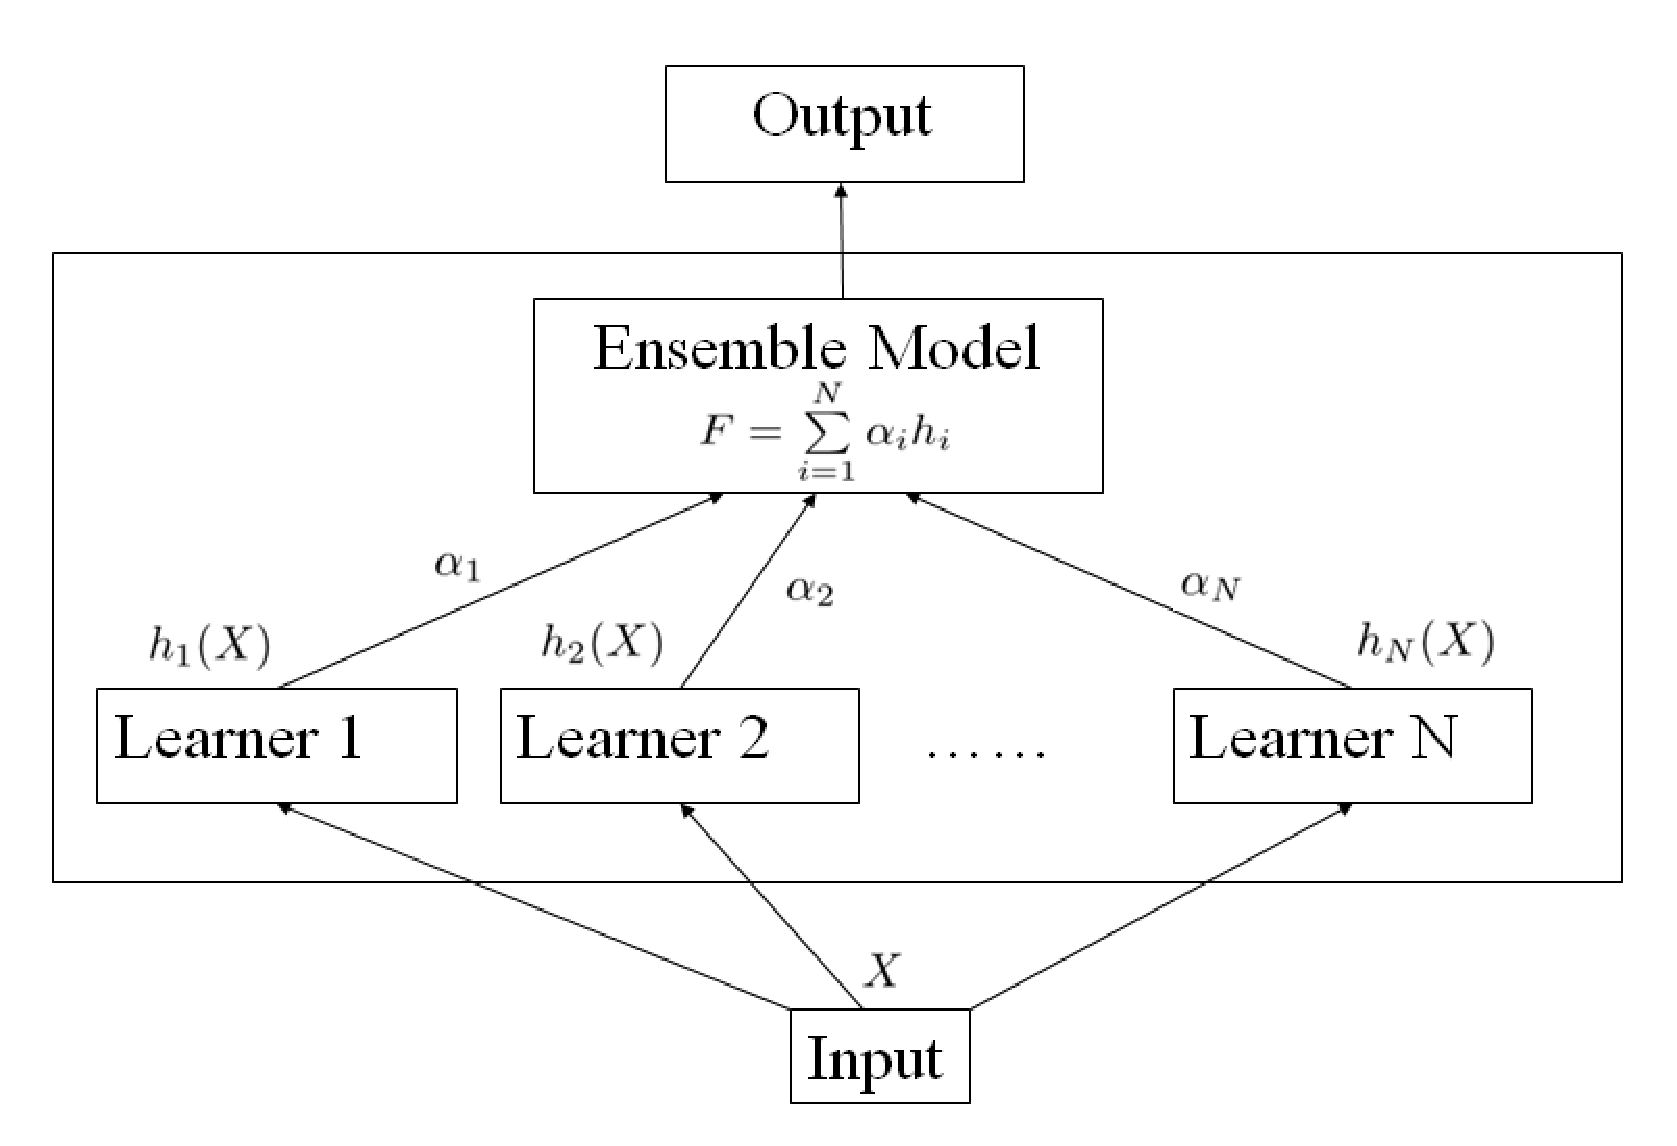
\includegraphics[width=0.6\textwidth,height=7cm]{figures/ensemblelearning.eps}\\
  \caption{集成学习框架}\label{fig:ensemblelearning}
\end{figure}

Thomas Dietterich\cite{dietterich2000ensemble}指出,集成学习有效可以归结于集成模型在统计、计算和模型表示三个方面的优势,认为集成模型能够有效地降低统计误差、优化误差和模型误差,那么构造出优良的集成模型自然水到渠成。

\begin{enumerate}[(1)]
  \item 统计的原因:一个学习算法就是从假设空间$\mathcal{H}$ 中寻找最佳的近似模型(假设),然而学习算法所使用的训练样本相对假设空间毕竟有限,假设空间中可能存在多个在训练集上精度相当的假设模型,构造集成模型要比选取单个模型更加明智,同时也免除了选择错误模型而带来的风险。
  \item 计算的原因:许多学习算法通常会陷于局部最优,通过增加训练样本,即便消除了统计误差,仍然不易找到全局最优的模型。每个假设模型实际上是从不同的初始点,不同的方向对真实函数的一种近似,集成模型的效果是大大降低单个模型的近似误差。
  \item 表示的原因:在实际应用中,也许假设空间$\mathcal{H}$ 中的任何假设都不能表示真实的函数$f$,那么通过加权形式集成的模型也就扩展了原始假设空间所表示的范围。
\end{enumerate}

在标准的监督学习问题中,给定训练数据集$S = \{x_i,y_i\}_{i=1}^n$,其中$x_i\in \mathbb{R}^m$是包含$m$个特征的样本,$y_i$表示样本的标记。假设样本特征$x$同样本标记$y$之间的真实关系是$y = f(x)$,或者说样本是从真实未知的分布$P(x,f(x))$ 中抽样得到。

假设当前学习的任务是训练一个分类器$h$,则分类器$h$就是未知函数$f$的一个假设。监督学习的目标是从训练数据集中学习出最佳模型$h\in \mathcal H$,从而使得损失函数的期望值最小:
\[
    h = \argmin\limits_{g\in \mathcal H} \mathbb E_{y,x} L(y,g(x))
\]
由于客观条件的限制,最终训练得到的模型还是会存在下面三种类型的误差(1)统计误差:由于真实函数未知,模型训练使用的训练集只能通过采样构建,并基于它最小化经验风险。(2)优化误差:优化损失函数的算法通常确定的是局部最优解,从而产生与全局最优解不一致的误差。(3)模型误差:监督学习建立在给定形式的模型上,或基于一定的先验概率,在模型空间的子空间中搜索,从而产生结构性的模型误差。集成学习的有效性分析,实际上就是分析集成模型降低统计误差、优化误差或模型误差的能力。

\ornamento
\section{多样性}\label{sec:diverisity}
假设集成分类器$F$包含$m$个基本分类器$\{h_i\}_{i=1}^m$,集成分类器的预测精度高于单个分类器的充分必要条件\cite{hansen1990neural}是:对于新的输入样本,单个分类器的预测精度要比随机猜测的高(Accurate),基本分类器间的预测误差具有差异性(Diverse)\cite{dietterich2000ensemble}。有研究表明,预测误差差异性的增加能够改善集成模型的性能:对于相同的输入,如果所有基本模型都给出相似的预测结果,则集成模型的泛化误差大于基本模型泛化误差的加权平均值;如果基本模型的预测误差存在较大的差异性,则集成模型的泛化误差远小于基本模型泛化误差的加权平均值。

A necessary condition for an ensemble to be more accurate than any of its individual members, is that the classifiers are accurate and diverse\cite{hansen1990neural}. An accurate classifier does better than random guessing on new examples. Two classifiers are diverse if they make different errors on new examples. There are several ways to introduce diversity: by \textbf{manipulating the training set} (by changing the weight of the examples\cite{breiman1996bagging,freund1996experiments} or by \textbf{changing the attribute values of the examples} \cite{breiman1999using}), or by \textbf{manipulating the learning algorithm itself} \cite{dietterich2000ensemble}.

目前,常见的增加集成模型误差多样性的方法包括:使用不同的训练集合(行采样、列采样)、使用不同类型的基本模型(模型结构、参数、初始化方式),整体而言可以分为同构(Homogeneous)与异构(Heterogeneous)模型两种。比如,Bagging、Boosting集成的基本模型是同构模型,Stacking集成的基本模型是异构模型。

Carbonell与Goldstein\cite{carbonell1998use}认为,评价信息检索的指标不仅要关注“检索相关性”(Query Relevance),还要考虑“信息新颖度”(Information Novelty)。他们引入“间隔相关性”(Marginal Relevance)的概念,兼顾相关性与新颖度,并充分考虑用户的个性化需求,通过灵活设置权衡参数,反映对二者的偏好程度。间隔相关性是相关性与新颖度的线性组合,选择备选文档的原则是最大化间隔相关性:
\begin{equation}\label{eq:mmr}
    \mathrm{MMR} = \argmax\limits_{d_i\in D\setminus S}\Big\{\lambda sim_1(d_i, q) - (1-\lambda) \max\limits_{d_j\in S}sim_2(d_i, d_j)\Big\}
\end{equation}
其中,$D$是文档集合,$S$代表已经选择的文档集,$q$表示检索词,$q_i,q_j$表示文档,$sim_1,sim_2$分别是文档-检索词相关性、文档-文档相似性的度量,$\lambda\in [0,1]$反映了对相关性偏好程度,比如当$\lambda=1$时,则仅仅以相关性为选择标准,当$\lambda = 0$,则新颖度是选择文档的主要依据。分析可以发现,如果备选文档同检索词相关程度越高,备选文档同已选文档之间的相似程度越低,则MMR越大。

由于精度-多样性两难问题(Accuracy-Diversity Dilemma),只有深入研究多样性同模型精度之间的密切关系,才能通过恰当的权衡获得最佳的性能。对此,多人已经作出深刻的分析\cite{cunningham2000diversity,kuncheva2003measures,tsymbal2005diversity}。 不同类型的多样性对于集成学习的影响也不同,
\cite{kuncheva2002experimental}中介绍了九种多样性度量,\cite{kuncheva2003measures}介绍了十种多样性度量。

\section{集成误差}
1992年,Stuart Geman等人\cite{geman1992neural}证明集成模型的预测误差可以分解为偏差、方差两部分(Bias-Variance分解)
\begin{equation}\label{eq:biasvariancedec}
    E (F - y)^2 = (E(F) - y)^2 + E(F- E(F))^2= \beta_F^2 + \sigma_F^2
\end{equation}
其中,$y$表示含有噪声的相应变量期望值,$F$表示集成模型,$\beta_F^2$表示它的预测偏差,$\sigma_F^2$表示集成模型的预测方差。图\ref{fig:bias-variance}形象解释了偏置与方差两个概念,偏置描述训练模型逼近真实模型的程度,而方差则反映训练模型忽略真实信号,学习随机事物的程度。

\begin{figure}[htbp]
  \centering
  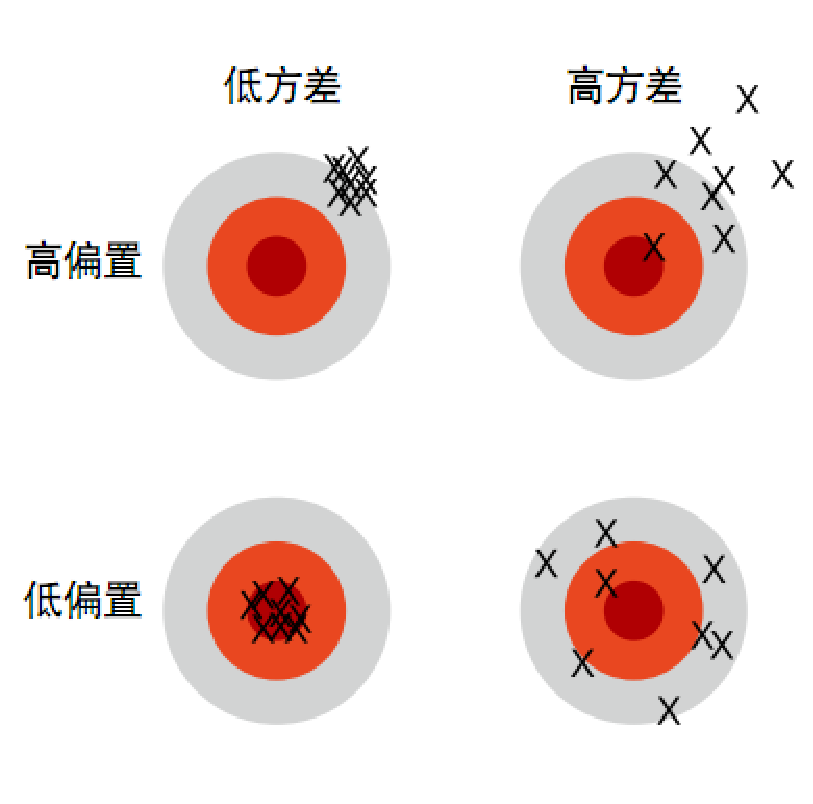
\includegraphics[width=0.45\textwidth,height=7cm]{figures/bias-variance.eps}
  \caption{飞镖投掷产生的偏置与方差}\label{fig:bias-variance}
\end{figure}

假设集成模型$F$是基本模型的凸组合:
\begin{equation}
    F= \sum\limits_i \omega_i h_i
\end{equation}
其中,$\omega_i$是基本模型$h_i$的权重,这里取$\omega_i=1/m$,$m$是基本模型的个数。

根据基本模型的平均偏差$\bar\beta_F^2$、平均方差$\bar\sigma_F^2$、平均协方差$\bar c_F$:
\begin{equation}\label{eq:averageq}
  \begin{array}{ll}
    \bar\beta_F^2 & =\frac{1}{m}\sum\limits_i (E(h_i) - y)^2 \\
    \bar\sigma_F^2 & =\frac{1}{m}\sum\limits_i E(h_i - E(h_i))^2\\
    \bar c_F & = \frac{1}{m(m-1)} \sum\limits_i \sum\limits_{j\neq i} E(h_i - E(h_i))(h_j - E(h_j))
  \end{array}
\end{equation}
分解方差项$\sigma_F^2$,从而将集成模型的预测误差分解成三个部分(Bias-Variance-Covariance分解)\cite{ueda1996generalization}:
\begin{equation}\label{eq:biasvariancecodec}
    E(F - y)^2 = E(\frac{1}{m} \sum\limits_i h_i - y)^2 = \bar\beta_F^2 + \frac{1}{m} \bar\sigma_F^2 + (1 - \frac{1}{m})\bar c_F
\end{equation}

1995年,Krogh和Vedelsby\cite{krogh1995neural}证明“集成模型的预测误差小于等于基本模型预测误差的加权平均值”(Ambiguity分解),具体地
\begin{equation}\label{eq:ambiguitydec}
    (F - y)^2 = \sum_i \omega_i(h_i - y)^2 - \sum_i \omega_i(F - h_i)^2 \le \sum_i \omega_i(h_i - y)^2
\end{equation}

Bias-Variance分解可以部分解释Boosting与Bagging集成技术的有效性,比如\cite{breiman1996bias}认为两者均能降低分类误差中的方差项,
\cite{freund1996experiments}则称Boosting能够降低分类误差中的偏差项。

\section{提升算法}
1984年,Leslie Valiant\cite{valiant1984theory}提出可能近似正确(Probably Approximately Correct,PAC)学习模型。
\footnote{Valint的PAC与Vapnik的统计学习理论(SLT),成为当今学习理论的主流,是使用最广泛的两种框架,并在实际中发展出经典的Boosting技术与SVM技术,1989 年,Anselm Blumer\cite{blumer1989learnability}等人首次将VC维与PAC联系起来。Leslie Valiant由此获得2010年的图灵奖,成为学习理论的先驱人物。}
1988年,Valiant与Kearns\cite{kearns1988learning}给出“强可学习”和“弱可学习”的概念:在PAC学习框架下,对于一个概念,如果存在一个多项式的学习算法,并且准确率很高,则称这个概念是\textbf{(强)可学习的},对应算法称为强学习算法;对于一个概念,如果存在一个多项式的学习算法,学习的准确率略高于随机猜测,则称这个概念是\textbf{弱可学习的},对应算法称为弱学习算法。与此同时,他们还提出一个开放性的问题:在PAC学习框架下,略好于随机猜测的弱学习算法能否提升为任意精度的强学习算法?如果可以,我们只要找到一种比随机猜测略好的弱学习算法就可将其提升为强学习算法,而不必费心设计出复杂的强学习算法。

1989年,Robert Schapire\cite{schapire1990strength}给出“强可学习与弱可学习等价”的数学证明,并设计出第一个多项式时间的Boosting算法;次年,Yoav Freund\cite{freund1990boosting}提出效率更高的“boost-by-majority”算法,但是两种算法都要求预先知道弱学习算法学习正确率的下限,给弱学习算法的选择设置了硬性的约束。1992年,Boosting首次用于提升神经网络模型OCR识别性能\cite{drucker1992improving,drucker1993boosting}。1995年,两人对“boost-by-majority”算法进行改进,提出了著名的AdaBoost算法(\textbf{Ada}ptive \textbf{Boost}ing)\cite{freund1995desicion}。两种算法效率相当,但AdaBoost没有对弱学习算法施加任何限制条件,更容易推广到实际应用。1999 年
\cite{schapire1999improved},两人引入置信分值的概念,将其扩展为广义的AdaBoost算法。目前,Boosting已经可以处理分类
\cite{freund1995desicion,friedman2000additive}、回归\cite{duffy2002boosting}与排序问题\cite{freund2003efficient,xu2007adarank}。

Boosting是一种典型的集成方法,其基本思想是通过迭代的方式构造弱学习器,依据弱学习器在训练集上的性能调整训练样本的权重,性能越高则权值越大,反之亦然,通过强化学习性能不佳的样例,构造出性能优良的集成模型。Boosting已经广泛应用到多个领域,如手写字符识别、图像识别及检索、文本分类、语音识别等。

对于稳定性差的学习算法,如决策树、决策树桩、神经网络,数据集的微小扰动都能明显改变学习的结果,Boosting倾向于使用它们作为弱学习算法,以增加误差产生的多样性,改善模型整体性能。
\subsection{AdaBoost}
AdaBoost算法对训练数据集每个样本赋以一个初始权值,迭代地添加弱分类器,并将选择的所有弱分类器组合作为最终的分类函数。在学习过程中,AdaBoost算法会实时调整样本权值,对当前分类函数正确分类的样本降低权值,而对错误分类的样本增加权重。
\begin{algorithm}[htbp]
        \caption{AdaBoost算法(二元分类)}
        \begin{algorithmic}
            \REQUIRE ~~训练集$S=\{x_i,y_i\}_{i=1}^n$,迭代次数$T$\\
            \STATE
            \begin{itemize}
              \item 初始化样本概率分布$P_1(i)=1/n,~~i=1,\ldots,n$
            \end{itemize}
            \FOR{$t = 1,\dots, T$}
            \STATE
            \begin{enumerate}
              \item 基于样本概率分布$P_t$训练弱学习器$h_t:X\mapsto \{-1,1\}$
              \item 计算弱学习器的分类误差
              \begin{equation}
                \epsilon_t = \sum\limits_{i=1}^n P_t(i) I(h_t(x_i)\ne y_i)
              \end{equation}
              \item 给弱学习器赋权值
                \begin{equation}
                    \alpha_t=\frac{1}{2}\log\frac{1-\epsilon_t}{\epsilon_t}
                \end{equation}
              \item 更新概率分布
              \begin{equation}
                P_{t+1}(i) = \frac{P_t(i) e^{-\alpha_t y_i h_t(x_i)}}{Z_t}
              \end{equation}
              其中,$Z_t$是标准化因子。
            \end{enumerate}
            \ENDFOR
            \ENSURE ~~最终分类模型$H(x) = \sgn\big(\sum\limits_{t=1}^T \alpha_t h_t(x)\big)$
        \end{algorithmic}
\end{algorithm}

\subsection{LPBoost}

\subsection{大间隔模型:提升算法}
1999年,Robert Freund与Yoav Schapire\cite{freund1999short}建立起Boosting同“间隔”的关系
\begin{equation}
    \rho = y f(x) = y \sum\limits_{t=1}^T \alpha_t h_t(x)\in [-1,1]
\end{equation}
其中,弱学习器$h_t$的权值$\alpha_t$为
\begin{equation}
    \alpha_t = \frac{1}{2} \log\frac{1-\sum\limits_i P_t(i) I\big[h_t(x_i)\ne y_i\big]}{\sum\limits_i P_t(i) I\big[h_t(x_i)\ne y_i\big]}.
\end{equation}

\subsection{提升算法的缺陷}
使用Boosting技术,能够在不依赖于先验知识的条件下,取得良好的预测性能。它也有缺点,比如在一定程度上依赖于训练数据集和弱学习器的选择,当训练数据小或弱学习器性能太差时,就会导致组合模型预测精度的下降。由于在迭代过程中,对噪声数据赋予了较大的权值,以增加其在后续迭代中的学习强度,从而对模型的收敛速度构成负面影响。如何选择合适的迭代次数,确定模型过拟合发生的条件,降低Boosting对噪声数据的敏感程度等,均是研究Boosting的重要课题。研究人员针对Boosting方法的缺陷陆续提出改进算法,经典的如Breiman\cite{breiman1998arcing}提出的Arching算法(Adaptive Re-sampling and Combining),Friedman等人\cite{friedman2000additive} 提出的LogitBoost 算法和Freund 的BrownBoost算法\cite{freund2001adaptive}。

\section{Bagging}
Bagging(\textbf{B}ootstrap \textbf{Agg}regat\textbf{ing})是第一个有效的集成学习算法,也是最简单的Arching(Adaptive Reweighting and Combining)方法,由Leo Breiman于1996 年发明\cite{breiman1996bagging}。 在Bagging 方法中,使用自举复制(Bootstrap Replicate)
\footnote{Bootstrap一说源自Rudolf Erich Raspe 的小说\textit{The Surprising Adventures of Baron Munchausen},主人翁Baron声称曾经揪着头发从沼泽中把自己拉出来,后来经过传播异化为拽着鞋带把自己拉起来(Pull oneself up by one's bootstraps),表示不可能完成的事。后来,计算机发明以后,机器的启动称为Boot,实际上就是Bootstrap的简写,因为计算机启动是一个很矛盾的过程:必须先运行程序,然后计算机才能启动,但是计算机不启动就无法运行程序。在统计学中,利用自举法构建新数据集的过程称为\textbf{重采样}(Resampling):从原始数据集进行多次\textbf{有放回}的采样,采样的次数等于原始数据集的大小。统计学中另外一种重采样方法是Jackknife,与Bootstrap类似,区别在它每次从样本中抽样时只是去除几个样本(而不是抽样),像小刀一样割去一部分。}
从原始数据集中产生多组新的训练集,利用这些具有差异性的数据集训练学习多个分类器,并根据多数表决方法,组合多个分类器对新样本分类。

Bagging算法的基本流程如下:
\begin{enumerate}
  \item 对原始训练集$X$,使用Boostrap方法复制构造$m$个大小与$X$相同\footnote{对于大型数据集,一般地要求每个抽样子集包含$1-1/e\approx 63.2\%$唯一样例}的训练集$S_1,S_2,\ldots,S_m$
  \item 对每个训练集$S_i$训练一个弱分类器$h_i$,$i=1,\ldots,m$
  \item 对于新的数据$x$,使用多数表决方法,综合所有弱分类器进行分类:
  \begin{equation}\label{eq:majorityvoting}
    \hat c = \argmax_{k=1,\ldots,K} n_k
  \end{equation}
  其中,$K$是分类的级别,$n_k$是预测$x$的类别为$c_k$的弱分类器个数:
  \begin{equation}
    n_k = \sum_{i=1}^m I(h_i(x) = k), k = 1,\ldots,K
  \end{equation}
\end{enumerate}

\begin{remark}
Bagging和Boosting的主要区别在于抽样方式不同,前者采用均匀抽样,而后者采用的方法在依赖于模型预测的错误率。Bagging随机选择训练集,各轮训练集之间相互独立;Boosting各轮训练集的选择与前面各轮的学习结果有关;Bagging各个预测函数没有权重,而Boosting 是有权重的;Bagging 的各个预测函数可以并行生成,而Boosting 的各个预测函数只能顺序生成。绝大多数情况,Bagging和Boosting都可以有效地提高分类的准确性,经验分析表明Boosting 略胜一筹
\cite{opitz1999popular}。
\end{remark}

\section{Stacking}
1992年,David Wolpert\cite{wolpert1992stacked}提出Stacking框架,也称“Stacking Generalization”。

\section{随机子空间法}
随机子空间法(Random Subspace Method,RSM或Attribute Bagging,AB)\cite{ho1998random,bryll2003attribute}是一种集成分类函数,属于随机森林算法的一般形式,不同的是随机森林由决策树组成,而随机子空间分类器是由任意基本分类器组成。随机子空间法已经被应用到线性分类、支持向量机、最近邻分类和其他类型的分类算法。

随机子空间法是在小样本高维度的训练数据集(小$n$大$p$)背景下提出来的,通过组合多个不同特征的分类器增加集成模型分类的互补性,对于改善模型性能大有裨益。

假设训练数据集中有$n$个样本,而每个样本的特征维数是$p$,随机子空间法的基本步骤如下:
\begin{enumerate}[(1)]
  \item 设定子空间的维度$p_0$以及弱分类器的个数$m$,一般地,$p_0 < p$。
  \item 对每个弱分类器$h_i$,从$p$个特征中不放回(Without Replacement)地选择$p_0$维特征,生成一个训练集,并训练分类器$h_i$。
  \item 对于新的样本,通过多数表决规则(Majority Voting Rule)或组合后验概率的方式,根据$m$个弱分类器的分类结果确定新样本的最终分类。
\end{enumerate}

\section{加性树丛模型}
加性树丛模型(Additive Groves,AG)~\cite{sorokina2007additive}由自举的加性模型(Bagged Additive Model)构成,以决策树为基本模型实现对非线性成分的拟合。由于它吸收了Bagging模型的思想,可通过增加迭代次数降低过拟合的风险,总体性能优于Bagging、Boosting、随机森林等决策树集成方法。
每个树丛都可以通过一组更小的树丛循环构建,从而能够在自举迭代过程,生出大小不一的一堆树丛。加性树丛模型含有两个参数:树的个数与树的大小。

\section{维数约减}
信息化技术的快速发展产生了大量高维非结构化的数据,在人脸识别、生物信息等领域,需要从高维数据中发现数据内在结构信息,并识别出本质特征。\textbf{维数约减}(Dimension Reduction),简称“\textbf{降维}”,也称\textbf{低秩近似}(Low-Rank Approximation)是处理高维数据的一种常用技术,将高维数据转至低维表达空间。

降维问题是在给定矩阵$A\in \mathbb R^{m\times n}$和数值精度$\epsilon>0$,搜索$A$的最佳近似矩阵$\hat A\in \mathbb R^{m\times n}$,即满足$\|A-\hat A\|_{\mathcal F} \le \epsilon \|A\|_{\mathcal F}$,并且在所有符合条件的矩阵集合内$\hat A$ 的\textbf{秩最小}。

\textbf{矩阵分解算法}(Matrix Factorization)是一类重要的降维工具,流行的分解算法包括LU分解(三角分解)、QR分解和奇异值分解(Singular Value Decomposition,SVD)、概率矩阵分解(Probabilistic Matrix Factorization,PMF)。\textbf{低秩模型}是高效处理高维数据的新工具,新近兴起的\textbf{稀疏表示}(Sparse Representation)和\textbf{压缩传感}(Compressed Sensing)在图像或视频压缩领域获得巨大成功,能够充分利用图像或视频的时空相关性,实现有效压缩。
\textbf{矩阵填充}(Matrix Completion)是一种特殊的低秩模型,它能够在矩阵数据部分缺失时,利用矩阵行列间的相关性恢复矩阵的低秩结构,广泛应用于机器控制、图像处理(如去噪)等领域。

\subsection{奇异值分解}
\textbf{奇异值分解}(简称SVD)是一种经典的矩阵分解方法,广泛应用于伪逆计算、信号处理,图像压缩、生物信息处理等工作。本文主要考虑实数矩阵上的分解问题。

\begin{proposition}
对于任意实数矩阵$A\in \mathbb R^{m\times n}$,矩阵$AA^T\in \mathbb R^{m\times m}$、$A^TA\in \mathbb R^{n\times n}$都是半正定矩阵,并且两者存在相同的非零特征值。假设矩阵$A^TA$的特征值是$\sigma_1^2\ge \sigma_2^2 \ge \ldots \ge \sigma_n^2\ge 0$,对应单位特征向量是$v_1, v_2,\ldots, v_n$。如果$m<n$,则$\sigma_1^2,\ldots, \sigma_m^2$也是矩阵$AA^T$的特征值,$AA^T$的对应单位特征向量是$u_1,u_2,\ldots, u_m$。如果以$u_1,u_2,\ldots,u_m$为列构成矩阵$U\in \mathbb R^{m\times m}$,以$v_1,v_2,\ldots, v_n$为列构成矩阵$V\in \mathbb R^{n\times n}$,以矩阵$A$的奇异值作为对角元的对角阵$\Sigma\in \mathbb R^{m\times n}$,则矩阵$A$可以直接表示成三个矩阵的乘积$A = U\Sigma V^T$,这种分解方法称作矩阵$A$的奇异值分解。
\end{proposition}

任意实数矩阵$A\in \mathbb R^{m\times n}$都可以分解成三个矩阵乘积的形式
\begin{equation}\label{eq:svd}
  A = U\Sigma V^T
\end{equation}
其中,$\Sigma \in \mathbb R^{m\times n}$是对角阵,$U\in \mathbb R^{m\times m}$,$V\in \mathbb R^{n\times n}$都是正交阵,即$UU^T = I_m, VV^T = I_n$。

如果将$\Sigma, U, V$分别展开,则有:
\begin{equation}
  U = (u_1,u_2,\ldots,u_m), u_i\in \mathbb R^m
\end{equation}

\begin{equation}
  V = (v_1,v_2,\ldots,v_n), v_j\in \mathbb R^n
\end{equation}

\begin{equation}
\Sigma =
\begin{bmatrix}
\sigma_1 & 0 & \cdots & 0 & 0 & \cdots & 0\\
0 & \sigma_2 & \cdots & 0 & 0 & \cdots & 0\\
0 & 0 & \ddots & 0 & 0 & \cdots & 0\\
0 & 0 & \cdots & \sigma_m & 0 & \cdots & 0
\end{bmatrix}
\end{equation}
这里假设$m<n$。

对于任意的$i\in\{1,\ldots,m\},j\in\{1,\ldots,n\}$,矩阵$U,V$ 的列向量$u_i,v_j$分别是$AA^T,A^TA$ 的特征向量,故称$u_i,v_j$ 为矩阵$A$的左、右奇异向量,$\Sigma$ 的对角元素$\sigma_i$称作矩阵$A$的奇异值,是$AA^T$或者$A^TA$特征值的算术平方根。不失一般性,假设$\sigma_1 \ge \sigma_2 \ge \ldots \ge \sigma_m$。

下文主要就这种关系给予简单证明。由于$A = U\Sigma V^T$,则$A^T = V\Sigma^T U^T$,那么
\begin{equation}
  A A^T = U\Sigma V^T V\Sigma^T U^T = U\Sigma\Sigma^T U^T =
U
\begin{bmatrix}
\sigma_1^2 & 0 & \cdots & 0\\
0 & \sigma_2^2 & \cdots & 0\\
0 & 0 & \ddots & 0\\
0 & 0 & \cdots & \sigma_m^2
\end{bmatrix}
U^T = \sum_{i=1}^m{\sigma_i^2 u_iu_i^T}
\end{equation}

类似地可得:
\begin{equation}
  A^T A = V\Sigma^T U^T U\Sigma V^T = V\Sigma^T \Sigma V^T = \sum_{j=1}^n{\sigma_j^2 v_jv_j^T}
\end{equation}

由此可得:
\begin{equation}
  A A^T u_k = \sum_{i=1}^m{\sigma_i^2 u_iu_i^T} u_k = \sigma_k^2 u_k
\end{equation}

\begin{equation}
  A^T A v_l = \sum_{j=1}^n{\sigma_j^2 v_jv_j^T} v_l = \sigma_l^2 v_l
\end{equation}
说明$u_k, v_l$分别是$AA^T,A^TA$的一个特征向量,对应的特征值分别是$\sigma_k^2,\sigma_l^2$。

SVD在实际使用时,通常仅仅选择最大的前$r$个奇异值以及$U,V$对应的$r$列向量,即可对矩阵$A$很好地近似:
\begin{equation}\label{eq:approxsvd}
    \tilde{A}_r = \sum_{i=1}^r{\sigma_i u_i v_i^T}
\end{equation}

可以证明,$\tilde{A}_r$是所有秩为$r$的$m\times n$矩阵中,与矩阵$A$最近似的矩阵。

观察$A$的分解式,可以发现:
\begin{equation}
    A = \sum_{i=1}^m{\sigma_i u_i v_i^T} = \sigma_1 u_1 v_1^T + \ldots + \sigma_m u_m v_m^T
\end{equation}
矩阵的$A$奇异值分解实际上是将其分解成一组秩为1的矩阵线性加权的形式,这里,奇异值是加权权值。从这个角度出发,我们在下文就SVD在推荐系统中的应用,介绍分解式中的矩阵$U,V$所代表的真实含义。

推荐问题通常都涉及到用户对物品的评价,从而构成系统评价矩阵$A\in \mathbb R^{m\times n}$,矩阵的行代表用户,列代表物品,通常由于用户的数目远远多于物品数量,所以有$m \gg n$。根据矩阵$U,V$的定义,它们的列向量是由$AA^T,A^TA$的(标准化的)特征向量构成。如果对评价矩阵行分块,即
\begin{equation}
  A =
    \begin{bmatrix}
        A_1\\
        A_2\\
        \vdots\\
        A_m
    \end{bmatrix}
\end{equation}
其中,$A_i\in \mathbb R^{1\times n}, 1 \le i \le m$,实际上代表一个用户评价向量。由此,可以得到
\begin{equation}
  AA^T =
    \begin{bmatrix}
        A_1\\
        A_2\\
        \vdots\\
        A_m
    \end{bmatrix}
(A_1^T, A_2^T, \ldots, A_m^T)
=
    \begin{pmatrix}
        A_1A_1^T & A_1A_2^T & \ldots & A_1A_m^T\\
        A_2A_1^T & A_2A_2^T & \ldots & A_2A_m^T\\
        \vdots & \vdots & \ddots & \vdots\\
        A_mA_1^T & A_mA_2^T & \ldots & A_mA_m^T
    \end{pmatrix}
\end{equation}

如果$A$的元素是多元评价等级,那么根据余弦相似度定义可知,$A_iA_j^T$代表用户$i,j$的评价向量内积,反映了二者之间的相似程度,如果$A$的元素是二元评价等级($0-$未评价,$1-$评价),则$A_iA_j^T$ 即是两个用户同时评价的物品数目,也是一种相似关系的度量,$AA^T$实际上就是用户群相似度矩阵。

由于矩阵$U$的列向量是由$AA^T$的标准特征向量构成,并且根据特征值与特征向量的统计学意义可知,特征值越大,对应特征向量方向上点的离散程度越高。不妨设想一下极端的情况,数据点只在两个维度(特征)上是不同的,在其他维度上数值完全一致,那么在其他维度上,点的离散程度为0,对于数据分类、聚类等任务,没有任何价值,相反,剩余两个维度是区分数据点的关键。也就是说,数据点的其他特征是冗余信息,将其删除百利而无一害。从信息熵的角度来看,混杂度越大(熵越大)的方向包含的信息量越大。

SVD的计算复杂度是$\complex(m^3 + n^3)$,在处理高维数据时会产生很大的问题。据悉,Google已经实现并行化SVD,可以扩大SVD实际应用的范围。

\begin{remark}
矩阵分解是对原始评分矩阵数据从多个维度所作的近似与还原,利用分解模型,可以构建项目间或用户间相似性矩阵(一阶或高阶),利用相似矩阵,可以进行对象的聚类分析,以簇或分组为单位可以显性地表示对象间的关系,对于理解隐语义模型内在机理大有裨益。此外,我们也可以直接从相似性矩阵的分块特征上与其他传统相似性度量进行比较和联系。我们还要思考:$AA^T$ 的特征向量同用户之间的关系?与$KNN$算法存在什么样的关联?
\end{remark}
\subsection{主成分分析}
假设多元随机变量$X = (X_1,\ldots, X_m)\in \mathbb R^{n\times m}$每个特征对应一个随机变量,每一行可以表示一个抽样数据。为了刻画特征之间的相关关系,我们可以计算所有特征序的相关系数,并构造$X$上的相关系数矩阵R。如果对原始数据逐列进行Z-Score标准化,不会影响到相关系数矩阵,则有
\[
    \bar X_1 = 0, ~~\var(X_1) = 1, ~~\text{R} = \frac{1}{n-1}X^T X.
\]
如果特征彼此间存在相关性,则会产生一定的冗余信息。为剔除冗余信息,1901年卡尔·皮尔逊Karl Pearson\cite{pearson1901liii}提出一种流行至今的线性降维方法:\textbf{主成分分析}(Principal Component Analysis,PCA)。如果多元随机变量,它利用一个特殊变换$A = (A_1, \ldots, A_m)\in \mathbb R^{m\times m}$ 重新组合原始特征集,构建出一组彼此线性无关的新特征$Y=(Y_1, \ldots, Y_m)\in \mathbb R^{n\times m}$。如果$A$满足性质
\begin{equation}
    \left\{
    \begin{array}{l}
        A_1 = \argmax\limits_{A_0}~ \var(XA_0),\\
        A_i = \argmax\limits_{A_0\perp \{A_j\}_{j=1}^{i-1}}~ \var(XA_0), 2 \le i \le m, \\
        \|A_i\|_2 = 1, 1\le i \le m.
    \end{array}
    \right.
\end{equation}
则称$A$是正交矩阵,相应地新特征
\begin{equation}
  Y_i = XA_i
\end{equation}
称作映射空间上的\textbf{第$i$个主成分},$1\le i\le m$。

\begin{proposition}
主成分相互独立,即对任意的$Y_i$与$Y_j$,都有相关系数$\rho(Y_i, Y_j) = 0$。此外,主成分和原始变量间满足相关关系$\rho(Y_i, X_j) = A_{ij}$。
\end{proposition}

\begin{proposition}
主成分方差顺次递减$\var(Y_1)\ge \var(Y_2)\ge \ldots \ge\var(Y_m)$,并且保持总方差不变,满足$\sum_{i=1}^m \var(Y_i) = \sum_{i=1}^m \var(X_i)=m$。
\end{proposition}

\begin{proposition}
假设$X$上的相关系数矩阵为R,则$A_i$是R的第$i$个特征向量,且对应特征值$\lambda_i = \var(Y_i)$,$1\le i\le m$,从而有$\lambda_1\ge \ldots \ge \lambda_m \ge 0$。
\end{proposition}

根据命题可知,主成分$Y$的方差值或相关系数矩阵R的特征值体现出原始数据的信息量,方差越大则所含信息量越大。在数据处理时,为了能够实现降维并确保最小化信息丢失,我们可以使用阈值法,比如设定一个百分比下限$\theta$,比如95\%,在前$K$个主成分的方差(相关系数矩阵R的$K$个最大特征值之和)占总方差(所有特征值之和)的比例超过$\theta$以后
\[
    \sum\limits_{i=1}^K \var(Y_i) \ge \theta \sum\limits_{i=1}^m \var(Y_i) = m \theta,
\]
则认定它们所包含的信息量足够高,从而可使用它们以近似表示原始高维空间
\begin{equation}\label{eq:pca-appr}
  \widehat Y = (Y_1,\ldots, Y_K) = X(A_1,\ldots,A_K)\in \mathbb R^{n\times K}, K \ll m.
\end{equation}

\subsection{局部线性嵌入}
局部线性嵌入(Locally linear Embedding,LLE)~\cite{belkin2001laplacian}是一种非线性降维方法,能够在降维后保持数据的原始流形结构,也是流形学习方法的一个经典工作。

\subsection{拉普拉斯特征映射}
拉普拉斯特征映射(Laplacian Eigenmaps)

\subsection{自组织映射网络}
自组织映射(Self Organizing Map,SOM)~\cite{kohonen1982self},也称自组织特征映射(Self Organizing Feature Map,SOFM)是由芬兰赫尔辛基理工大学教授Teuvo Kohonen发明的一种特殊的神经网络结构,通过无监督学习将输入样本映射至低维表示空间(二维或一维),并能保持原有数据的拓扑结构。

\subsection{自适应交叉近似算法}
自适应交叉近似算法(Adaptive Cross Approximation,ACA)是由Bebendorf和Rjasanow\cite{bebendorf2003adaptive}共同提出的一种低秩分解算法,首先将边界元(Boundary Element)矩阵分成若干块,然后对每一块(不包括对角线附近的块)做低秩分解。

传统边界元方法使用的系数矩阵$A$是满秩的,其中$A$中的每个元素都需要显式存储和参与运算。ACA算法的基本原理是:通过树状结构递归地将$A$分解为一系列子矩阵$A_{m_i\times n_i}^i$的集合,每个子矩阵对应$m_i$ 个源点和$n_i$个场点,当源点集合和场点集合距离足够远,则$A_{m_i\times n_i}^i$的秩很低,从而可以使用一组向量内积的和进行低秩近似:
\begin{equation}\label{eq:aca}
  A_{m_i\times n_i}^i \approx \sum_{l=1}^k{U_lV_l^T}
\end{equation}
其中,向量$U_l\in \mathbb R^{m_i},V_l\in \mathbb R^{n_i}$;$k$表示向量的个数,与低秩近似残差阈值$\epsilon$有关,通常$k\ll m_i$,$k\ll n_i$。由此可见,通过ACA低秩近似,对原子矩阵$A_{m_i\times n_i}^i$的存储量从$\complex(m_i n_i)$降低至$\complex[k(m_i + n_i)]$,并且在进行矩阵-向量乘积时,能够减少运算量。假设向量$X\in \mathbb R^{n_i}$
\begin{equation}
  A_{m_i\times n_i}^i X \approx (\sum_{l=1}^k{U_lV_l^T})X = \sum_{l=1}^k{w_lU_l}
\end{equation}
由此可见,矩阵-向量乘积问题就转化为简单的线性加权问题,权值为$w_l = V_l^TX,l=1,\ldots,k$,近乎线性复杂度。

\section{特征选择}
从理论上来看,特征越多则提供的信息也就越多,但是,现实世界表明,该论断并非总是成立的。特征选择(Feature Selection)有时又称特征子集选择(Feature Subset Selection,FSS)或者属性选择(Attribute Selection)
\footnote{苍梧:\href{http://www.cnblogs.com/heaad/archive/2011/01/02/1924088.html}{特征选择常用算法综述}},
属于机器学习预处理过程,通过降低数据的维数、剔除噪声数据和冗余特征,能够有效改善模型的学习精度与泛化能力,提高训练模型的效率。

%特征选择与基于映射的主成分分析,基于信息理论的维数约减技术不同,它不改变变量的原始表示。

目前,大多数特征选择的方法用于分类问题,基本上可分为三类\cite{guyon2003introduction}:过滤模式(Filter Method)\cite{mladenic1999feature}、包装模式(Wrapper Method)\cite{breiman1984classification}和嵌入模式(Embedded Method)\cite{kohavi1997wrappers}。

过滤模式将特征选择视为预处理步骤,与分类模型无关。它对每个特征计算一个相关性分值,分值低的特征将从特征空间中剔除。过滤模式易于扩展到高维特征数据,计算效率高、开销小,与具体分类模型无关。在过滤模式中,特征子集的搜索独立于模型假设空间上的搜索,并且在计算特征的相关性时,独立分析,忽视了特征之间的依存关系(Feature Dependency)。过滤模式存在两个代表性的模型:Relief 算法\cite{kira1992practical} 和Focus 算法\cite{almuallim1991learning}。

包装模式在特征子集的搜索过程,训练分类模型,使用一个预测模型给特征子集评分。包装模式对每个特征子集训练一个分类模型,模型在测试集上的预测误差用以衡量特征子集。随着特征数目的增大,特征子集的数目呈指数增加。为了搜索整个特征空间,人们陆续提出多种启发式搜索方案以搜寻最优特征子集。由于包装模式对于每个特征子集都需要训练一个预测模型,计算成本较高,并且容易产生过拟合问题。

嵌入模式在模型选择(训练、搜索)的同时选择最佳特征子集,将特征选择直接内嵌到到学习算法。与包装模式相比,嵌入模式的计算开销更小。典型的嵌入模式特征选择算法是决策树算法,如Quinlan的ID3、C4.5\cite{quinlan1986induction,quinlan1993c4}和Breiman的CART算法\cite{breiman1993classification}等,在树增长的过程,每个递归步骤都必须选择一个特征,将样本集合划分成更小的子集,选择特征的依据通常是划分以后子节点的纯度,子节点越纯则表明划分效果越佳,可见决策树生成的过程就是特征选择的过程。

\subsection{Relief}
1992年,Kira和Rendell提出了著名的Relief算法\cite{kira1992practical},它属于一种特征加权算法(Feature Weighting Algorithm),根据各个特征与类别的相关性赋予不同的权重,如果权重小于给定的阈值则将其剔除。

\subsection{贪婪搜索算法}
从整个特征空间选择特征,主要依赖两个指标:特征的重要程度、特征间的相似性。特征的重要程度容易计算,只要将单个特征独自作为一个排名模型,特征值便是预测结果,同真实相关等级比对,计算MAP、NDCG等评价指标立时可以作为特征的重要性权值。根据特征间的相似性,可以决定哪些特征可选,哪些特征冗余。但凡与已选特征高度相似的,即可认定是冗余特征,反倒是那些差异较大的特征,对于排序模型性能的提升多有裨益。计算相似性分值的指标很多,可以是余弦相似度,也可以是肯德尔距离。

假设特征空间$\mathcal F$含有$d$个特征:$\mathcal F = \{f_1, \ldots, f_d\}$,\cite{geng2007feature}通过下面的优化问题选择特征:
\begin{equation}\label{eq:mfeatureselect}
    \begin{array}{ll}
      \max\limits_a & \sum\limits_{i = 1}^d \omega_i a_i\\
      \min\limits_a & \sum\limits_{i = 1}^d \sum\limits_{j \ne i} s_{ij} a_i a_j\\
      \textit{s.t.} & a_i\in \{0, 1\}, i = 1,\ldots, d\\
      & \sum\limits_{i=1}^d a_i= m
    \end{array}
\end{equation}
其中,$a = (a_1,\ldots,a_d)$表示特征选中与否的标识,如果特征(比如$f_i$)被选中,则$a_i = 1$,否则$a_i = 0$;$\omega_i$表示特征$f_i$的权重;$s_{ij}$表示特征$f_i, f_j$的相似度,并且满足$s_{ij} = s_{ji}$;$0 < m \le d$是预先设置的入选特征的个数。

模型\eqref{eq:mfeatureselect}是个多目标优化问题,为方便计算,将其转化为单目标优化问题:
\begin{equation}\label{eq:featureselect}
    \begin{array}{ll}
      \max\limits_a & \sum\limits_{i = 1}^d \omega_i a_i - \lambda\sum\limits_{i = 1}^d \sum\limits_{j \ne i} s_{ij} a_i a_j\\
      \textit{s.t.} & a_i\in \{0, 1\}, i = 1,\ldots, d\\
      & \sum\limits_{i=1}^d a_i= m
    \end{array}
\end{equation}
模型中,参数$\lambda >0$是权衡特征重要程度与特征相似度的因子。

由于时间复杂度高达$\complex(\binom{d}{m})$,使用穷举法求解\eqref{eq:featureselect}是不现实的,自然需要构思高效的求解方法,比如Geng等人使用\textbf{贪婪搜索算法}(Greedy Search Algorithm,GSA)将时间复杂度降至$O(dm)$\cite{geng2007feature}。
\begin{algorithm}[htbp]
        \caption{GSA: Greedy Search Algorithm of Feature Selection}
        \begin{algorithmic}[1]
           \REQUIRE ~~\\
            使用特征集合$\mathcal F$中全部特征作为结点,构造无向图$G$,图中每条边的权值表示边的两个特征结点的相似度;$S$表示选中的特征集,并初始化为$S = \phi$;给定单目标优化中使用的参数$\lambda$。
            \FOR{$t = 1,\dots, m$}
            \STATE 从$G$中选取权值最大的特征结点,记为$f_{k_t}$
            \STATE 根据$f_{k_t}$与其他结点的相似度,惩罚其余诸结点,更新它们的权重:
            \[ \omega_i \leftarrow \omega_i - 2\lambda s_{ik_t}, i \ne k_t\]
            \STATE 将特征$f_{k_t}$添加至$S$中,并从$G$中剔除与结点$f_{k_t}$有关联的边:
            \[ S \leftarrow S \bigcup \{f_{k_t}\}, G \leftarrow G \setminus \{f_{k_t}\} \]
            \ENDFOR
            \ENSURE $S_m$\\
        \end{algorithmic}
\end{algorithm}

下面我们证明\cite{geng2007feature}:在不改变已入选特征的条件下,GSA能够找到\eqref{eq:featureselect}的最优解。

\begin{proof}
假设经过$t$次迭代,入选的最优特征集合$S_t = \{f_{k_i}\}_{i=1}^t$,未入选的某个结点$f_j$权值为
\begin{equation}\label{eq:weightupdate}
  \omega_j - 2\lambda \sum\limits_{i=1}^t s_{{k_i},j}
\end{equation}

根据GSA的目标函数,在第$t+1$次迭代,基于如下原则选出最佳特征:
\begin{equation}\label{eq:bestselect}
    \max~~\sum\limits_{i=1}^{t+1} \omega_{k_i} - \lambda \sum\limits_{i=1}^{t+1}\sum\limits_{j\ne i} s_{k_{t_i}k_{t_j}}
\end{equation}

由于$s_{k_{t_i}k_{t_j}} = s_{k_{t_j}k_{t_i}}$,则有$\sum\limits_{i=1}^{t+1}\sum\limits_{j\ne i} s_{k_{t_i}k_{t_j}} = 2\sum\limits_{i=1}^{t}\sum\limits_{j = i+1}^{t+1} s_{k_{t_i}k_{t_j}}$,则目标函数可分解为两部分:
\begin{equation}
  \bigg\{\sum\limits_{i=1}^t \omega_{k_i} - 2\lambda \sum\limits_{i=1}^{t-1}\sum\limits_{j = i+1}^t s_{k_{t_i}k_{t_j}}\bigg\} + \bigg\{\omega_{k_{t+1}} - 2\lambda \sum\limits_{i=1}^t s_{k_{t_i}k_{t+1}}\bigg\}
\end{equation}
第一部分是常数,因此,\eqref{eq:bestselect}等价于如下的优化问题:
\begin{equation}\label{eq:lastselect}
    \max~~\omega_j - 2\lambda \sum\limits_{i=1}^t s_{k_{t_i},j}
\end{equation}
可见,GSA搜索方法确能找到\eqref{eq:featureselect}最优解。\qedhere
\end{proof}

GAS属于过滤模式的特征选择方法,作为预处理步骤,其效果需要使用具体的排名模型予以检验。\cite{geng2007feature}使用SVMRank与RankNet两种模型试验发现,相比基准的特征选择方法信息增益(Information Gain, IG)与卡方(Chi-square,CHI),GAS表现突出。如果数据集中各个特征的表现存在明显的差异,利用特征的重要性最大化、特征间相似性最小化的原则选择特征,可以有效消除噪声的影响,效果提升相当显著。

GAS在构建无向图$G$时,需要计算所有特征对的相似度,如果数据集是高维特征,会产生大量的计算开销,制约其扩展能力。\cite{yu2009efficient} 借鉴用于分类特征提取的Relief 算法\cite{kira1992practical}提出两种特征选择模型:RankFilter与RankWrapper,扩展性能较之GAS更佳,并且计算效率较高。

\subsection{FS-BFS}
FS-BFS(Feature Selection-Best First Search)属于包装模式的特征选择方法\cite{dang2010feature},先使用Best First搜索方法把特征空间划分成$k$ 个互不相交的特征子集,再应用坐标下降法(Coordinate Descent)给特征子集赋权。FS-BFS计算开销较大,因此对于大数据集,扩展性欠缺。

\chapter{推荐系统}
传统搜索算法只能呈现给所有的用户相同的搜索结果,无法针对用户的兴趣偏好提供个性化的服务,这种在信息爆炸时信息的利用率反而降低的现象称为\textbf{信息过载}
(Information Overload)。个性化推荐,包括个性化搜索,被认为是当前解决信息过载问题最有效的工具之一。推荐是一种特殊形式的\textbf{信息过滤}
(Information Filtering),通过挖掘用户历史行为、用户间或物品间的相似关系,给网络终端用户提供符合其个性偏好的信息列表。

推荐系统是一种网络应用,可以代替用户评估其从未看过的产品,如书籍、电影、网页、酒店、音乐等,推荐经过一个从已知信息中学习,然后对未知世界进行预测的过程。一个完整的推荐系统由三个部分组成:收集用户信息的行为记录模块,分析用户偏好的模型分析模块和推荐算法模块。行为记录模块负责记录用户的偏好行为,如评价、购买、浏览、问答、下载等。模型分析模块的主要目标是使用用户行为记录模块的信息构造出用户的潜在兴趣模型。推荐算法模块则是利用后台推荐算法实时地从产品集合中筛选出用户感兴趣的产品,生成推荐列表给用户。

根据推荐算法的不同,推荐系统大致可以分成三类:\textbf{协同过滤推荐系统}、\textbf{基于内容的推荐系统}、\textbf{混合推荐系统}。

\ornamento
\section{协同过滤}
协同过滤系统是第一代被提出并得到广泛应用的推荐系统,其核心思想可以分成两部分:1)利用用户历史行为数据计算用户之间的相似性,2)根据与目标用户相似性高的用户集合(邻域)对其他物品的评价数据,预测目标用户对未知对象的偏好程度,并以此对目标用户进行推荐。协同过滤系统最大的优点是对推荐对象没有特殊的要求,它能处理音乐、电影等难以进行文本结构化表示的对象。另一方面,协同过滤系统也面临几个重要的问题:冷启动(Cold Start)、稀疏性(Sparsity)和可扩展性
(Scalability)。

协同过滤系统的算法大致可以分成两类:\textbf{基于记忆的(Memory-based)}和\textbf{基于模型(Model-based)的推荐算法}。在协同过滤系统中,建立用户与物品之间关系最常见的方式就是评分,给定一个用户,系统中物品与给定用户的关系无非是已经评价或没有评价两种。基于记忆的协同过滤系统的目标是利用系统中历史评价信息,通过用户之间或者物品之间的相似关系,预测指定用户对于未评价物品的偏好程度,从而可能给出的评分。如果系统利用的是用户之间的相似关系进行协同过滤推荐,则称此系统为\textbf{基于用户的协同过滤系统(简称UserCF)};反之,如果利用物品之间的相似关系进行预测,则称其为\textbf{基于物品的协同过滤算法(简称ItemCF)}。

我们定义如下基本的数学符号,将在本章统一使用它们:
\begin{itemize}
  \item $\mathcal U$ - 用户集合
  \item $\mathcal I$ - 物品集合
  \item $A = (r_{ui})_{m\times n}$ - 用户对物品的评分矩阵
  \item $r_{ui}$ - 用户$u$对项目$i$的历史评分
  \item $p_{ui}$ - 用户$u$对项目$i$的模型预测评分
  \item $z_{uv}$ - 如果项目集中存在至少一个项目由用户$u$和$v$ 共同评价过,则$z_{uv}=1$;否则,$z_{uv}=0$
  \item $z_{ij}$ - 如果用户集中存在至少一名用户既评价过项目$i$ 又评价过项目$j$,则$z_{ij}=1$;否则,$z_{ij}=0$
  \item $z_{ui}$ - 如果用户$u$评价过项目$i$,则$z_{ui}=1$;否则,$z_{ui}=0$
  \item $\mathcal U_i$ - 评价过物品$i\in \mathcal I$的用户集合,$\mathcal U_i=\{u\in \mathcal U|z_{ui}=1\}$
  \item $\mathcal I_u$ - 系统推荐给用户$u$或$u$评价过的商品集合,$\mathcal I_u=\{i\in \mathcal I|z_{ui}=1\}$
  \item $\mathcal U_{ij}=\mathcal U_i \bigcap \mathcal U_j=\{u\in\mathcal U|z_{ui}=z_{uj}=1\}$ - 既评价过物品$i$ 又评价过物品$j$ 的用户集合
  \item $\mathcal I_{uv}=\mathcal I_u \bigcap \mathcal I_v=\{i\in\mathcal I|z_{ui}=z_{vi}=1\}$ - 系统推荐给用户$u$和$v$相同的物品集合或两者均评价过的物品集合
  \item $\bar r_u = \frac{1}{|\mathcal I_u|} \sum\limits_{i\in\mathcal I_u} r_{ui}$ - 用户历史平均评分
  \item $\bar r_i = \frac{1}{|\mathcal U_i|} \sum\limits_{u\in\mathcal U_i} r_{ui}$ - 物品历史平均得分
  \item $s_{uv}$ - 用户$u\in \mathcal U$和$v\in \mathcal U$ 的相似度
  \item $s_{ij}$ - 物品$i\in \mathcal I$和$j\in \mathcal I$ 的相似度
  \item $\mathcal N(u;\kappa)$ - 用户集中与用户$u\in \mathcal U$相似度最高的$\kappa$名用户,也称用户$u$的$\kappa$近邻
  \item $\mathcal N(i;\kappa)$ - 物品集中与物品$i\in \mathcal I$相似度最高的$\kappa$个物品,也称物品$i$的$\kappa$近邻
\end{itemize}

在协同过滤计算时,建立用户间或项目间的相似度关系是重要的一环。目前,使用最多的相似性度量主要是余弦相似度(Cosine Similarity)、修正的余弦相似度(Adjusted Cosine Similarity)和皮尔逊相关系数(Pearson Correlation Coefficient)。给定项目$i$与$j$,两者之间的余弦相似度为评分矩阵$A$中$i$列和$j$列评分向量的余弦值:
\begin{equation}
    s_{ij} = \frac{\sum\limits_{u\in \mathcal U} r_{ui} r_{uj}}{\sqrt{\sum\limits_{u\in \mathcal U} r_{ui}^2}\sqrt{\sum\limits_{u\in \mathcal U}r_{uj}^2}}.
\end{equation}
余弦相似度度量的相似度存在一个重要的缺陷,它没有考虑到不同用户的评分尺度的差异。对于同一个项目,部分用户评分偏高,而部分用户评分又可能偏低。为了弥补这一缺陷,研究人员对余弦相似度度量进行修正,对每个评分减去对应用户的平均评分量,然后再计算项目之间的相似度:
\begin{equation}
    s_{ij} = \frac{\sum\limits_{u\in \mathcal U_{ij}} (r_{ui} - \bar r_u) (r_{uj} - \bar r_u)}{\sqrt{\sum\limits_{u\in \mathcal U_{ij}} (r_{ui}-\bar r_u)^2}\sqrt{\sum\limits_{u\in \mathcal U_{ij}}(r_{uj}-\bar r_u)^2}},
\end{equation}
其计算仅限于共同评价过两个项目的用户。

在基于物品的协同过滤推荐中,使用修正的余弦相似性度量物品间的相似性更佳,然而在基于用户的协同过滤推荐中皮尔逊相关系数更为有效~\cite{jannach2010recommender}。对于用户$u$和$v$,两者的历史平均评分分别是$\bar r_u$ 和$\bar r_v$,则有
\begin{equation}
    s_{uv} = \frac{\sum\limits_{i\in \mathcal I_{uv}} (r_{ui} - \bar r_u) (r_{vi} - \bar r_v)}{\sqrt{\sum\limits_{i\in \mathcal I_{uv}} (r_{ui}-\bar r_u)^2}\sqrt{\sum\limits_{i\in \mathcal I_{uv}}(r_{vi}-\bar r_v)^2}},
\end{equation}
其计算与修正的余弦相似度类似,仅仅限于用户$u$和$v$共同评价过的项目集$\mathcal I_{uv}$。

\subsection{基于用户的协同过滤算法}
基于用户的协同过滤算法(User-based Collaborative Filtering)根据用户之间的相似性关系,间接地预测用户$u$对物品$i$的可能评分。我们结合皮尔逊相关性度量方法,可以建立如下形式的预测模型:
\begin{equation}
    p_{ui} = \bar r_u + \frac{\sum\limits_{v \in \mathcal U_i} \gamma_{uv} (r_{vi} - \bar r_v)}{\sum\limits_{v \in \mathcal U_i} |\gamma_{uv}|},
\end{equation}
其中,$\gamma_{uv}=s_{uv}|s_{uv}|^{\rho-1}$是关于皮尔逊相关性的一种转换,以降低噪声数据对预测的干扰。实验
\cite{breese1998empirical,lemire2005slope}表明$\rho=2.5$时,可以取得不错的效果。

由皮尔逊相关性分析可知,可能存在相当比例的用户与用户$u$没有太大的相关性。为此,研究人员在相似度度量的基础上,从用户集中筛选出部分与用户$u$相关性强的用户参与运算。比如,择出最相似的部分用户$\mathcal N(u; k)$,利用它们对物品$i$的历史评分数据,基于如下公式估计用户$u$对物品$i$的评分:
\begin{equation}\label{eq:ucf}
    p_{ui} = \bar r_u + \frac{\sum\limits_{v \in \mathcal N(u; k)} s_{uv} (r_{vi} - \bar r_v)}{\sum\limits_{v \in \mathcal N(u; k)} |s_{uv}|}.
\end{equation}

\subsection{基于物品的协同过滤算法}
基于物品的协同过滤算法\cite{sarwar2001item,bell2007scalable} (Item-based Collaborative Filtering)预测用户$u$对物品$i$的评分,最基本的形式是使用用户$u$ 对物品$i$ 相似的其他物品评分的加权平均值作为预测值\cite{jannach2010recommender}
\begin{equation}\label{eq:icf}
    p_{ui} = \frac{\sum\limits_{j \in \mathcal N(i; k)} s_{ij} r_{uj}}{\sum\limits_{j \in \mathcal N(i; k)} |s_{ij}|},
\end{equation}
其中,$\mathcal N(i; k)$表示与物品$i$相似度最高的$k$个物品所构成的近邻集合。

\section{Slope One}
协同推荐算法最基本的是基于用户的协同推荐和基于物品的协同推荐算法,在处理海量数据时,由于计算量大,扩展性容易遭遇瓶颈。为此,研究人员提出许多基于模型的协同过滤算法,根据评价数据推断和学习用户的行为模型,实现高效的预测评分。2005年,Daniel Lemire 和Anna Maclachlan~\cite{lemire2005slope}提出Slope One,它是一种新颖的基于模型的评分预测模型,在处理海量数据时依然可以保证良好的运算速度与推荐效果。目前,研究人员已经将其引入到其他模型
\cite{gao2009personalized,wang2009personalized,zhang2009item,sun2011one},以改善推荐系统的推荐精度,并成为各种在线推荐系统的一个重要算法。

Slope One算法从拟合一个单变量线性回归模型出发,在不需要计算项目间或用户间相似度的基础上,确立一种评分预测的策略。假设我们使用训练集$\{x_i, y_i\}_{i=1}^n$拟合一个简单的线性回归模型$f(x)=x+b$,则根据预测误差平方和最小化,我们可以确定最佳的参数$b^*$
\begin{equation}
    b^* = \argmin\limits_{b\in \mathbb R} \frac{1}{n}\sum\limits_i \big[f(x_i) - y_i\big]^2 = \frac{1}{n}\sum\limits_i (y_i-x_i).
\end{equation}
对于新的输入数据$x_0$,我们可以利用训练得到的模型$f(x)=x+b^*$ 进行预测$y_0=f(x_0)=x_0+\sum\limits_i(y_i-x_i)/n$。如果将推荐系统所有存在共同评价用户的项目评分组成训练集$\{r_{vi},r_{vj}\}_{i,j\in \mathcal I}^{v\in \mathcal U_{ij}}$,则可以建立一种简单的线性评分预测模型。如果用户$u$只评价过项目$j$,且项目对$(i,j)$存在共同评价用户,则模型预测用户$u$对项目$i$ 的评分只依赖于他对项目$j$的历史评分、项目对$(i,j)$ 的平均评分差值
\begin{equation}
    p_{ui} = r_{uj} + \frac{1}{|\mathcal U_{ij}|} \sum\limits_{v\in \mathcal U_{ij}} (r_{vi} - r_{vj}) = r_{uj} + \delta_{ij},
\end{equation}
其中,$\delta_{ij}$为项目对$(i,j)$的平均评分差值。如果用户$u$ 评价过的项目很多,并且能够与项目$i$存在共同的评价用户,那么模型的预测就建立在所有这些历史评分的基础之上
\begin{equation}\label{eq:slopeone}
    p_{ui} = \frac{1}{|\mathcal Z_{ui}|} \sum\limits_{j\in \mathcal Z_{ui}} (r_{uj} + \delta_{ij}).
\end{equation}
集合$\mathcal Z_{ui}=\{j\in \mathcal I_u|z_{ij}=1, j\ne i\}$ 是用户$u$评价过的且与$i$享有共同评价用户的项目集合。如果评分矩阵足够稠密,则$\mathcal Z_{ui}\approx \mathcal I_u$,由此我们可以取得其近似值
\begin{equation}
    p_{ui} \approx \bar r_u + \frac{1}{|\mathcal Z_{ui}|} \sum\limits_{j\in \mathcal I_u} \delta_{ij}.
\end{equation}

\subsubsection{加权Slope One}
在实际应用中,系统中不同项目的评分数量可能存在较大差异。比如,系统中有10,000名用户曾经评价过项目对$(i,j)$,却只有区区200名用户评价过项目对$(j,k)$,显然项目对评分数量的巨大差异一定会影响到Slope One模型在预测时的偏倚。为此,Daniel Lemire 和Anna Maclachlan~\cite{lemire2005slope}利用项目对评价的数量对Slope One 进行改进,提出一种加权型的Slope One算法
\begin{equation}\label{eq:weightedslopeone}
    p_{ui} = \frac{1}{\sum\limits_{j\in \mathcal I_u\setminus \{i\}} |\mathcal U_{ij}|} \sum\limits_{j\in \mathcal I_u\setminus \{i\}} (r_{uj} + \delta_{ij})|\mathcal U_{ij}| .
\end{equation}

\subsubsection{Bi-Polar Slope One}
从数值上来看,用户对项目的评分越高表明对项目越喜欢,反之则不喜欢。然而,不同的用户对于同一个项目,可能由于个人偏好、性格的差异,相同的评分所表达的好恶强度亦有所不同。譬如,一个天性乐观的人,在评分时可能偏高,即便有些项目并非其所好,其评分可能让然会高于绝大多数评分。为了更准确地衡量其喜恶,我们可以根据其历史评分信息,对所有其打过分的项目进行划分:如果项目的得分高于用户的平均历史评分,则说明用户喜欢此项目,反之则认定其不喜欢。用户对项目的喜欢与否亦有助于我们对用户进行分组,从而建立一个更佳的预测模型。

我们假设某用户$u$喜欢的项目集为$\mathcal I_u^{+}=\{i\in\mathcal I_u|r_{ui}>\bar r_u\}$,不喜欢的项目集为$\mathcal I_u^{-}=\{i\in\mathcal I_u|r_{ui}<\bar r_u\}$。对于任意项目对$(i,j)$,我们可以划出两类特殊的用户组:两个项目都喜欢$\mathcal U_{ij}^{+}=\{u\in \mathcal U|i, j\in \mathcal I_u^{+}\}$,两个项目都不喜欢$\mathcal U_{ij}^{-}=\{u\in \mathcal U|i, j\in \mathcal I_u^{-}\}$。对于同一个项目对具有相同喜恶观念的评分对于预测评分更有价值,对应地可以计算出Slope One模型基础上的两组平均评分差值
\begin{eqnarray}
  \delta_{ij}^{+} &=& \frac{1}{|\mathcal U_{ij}^{+}|}\sum\limits_{u\in \mathcal U_{ij}^{+}} (r_{ui} - r_{uj})\\
  \delta_{ij}^{-} &=& \frac{1}{|\mathcal U_{ij}^{-}|}\sum\limits_{u\in \mathcal U_{ij}^{-}} (r_{ui} - r_{uj})
\end{eqnarray}
基于此,我们使用加权型Slope One可以建立下面形式的预测模型:
\begin{equation}\label{eq:bipolarslopeone}
    p_{ui} = \frac{1}{\sum\limits_{j\in \mathcal I_u^{+}\setminus \{i\}} |\mathcal U_{ij}^{+}|+\sum\limits_{j\in \mathcal I_u^{-}\setminus \{i\}} |\mathcal U_{ij}^{-}|} \bigg\{\sum\limits_{j\in \mathcal I_u^{+}\setminus \{i\}} (r_{uj} + \delta_{ij}^{+})|\mathcal U_{ij}^{+}| + \sum\limits_{j\in \mathcal I_u^{-}\setminus \{i\}} (r_{uj} + \delta_{ij}^{-})|\mathcal U_{ij}^{-}| \bigg\}.
\end{equation}

\section{Baseline}
协同过滤模型试图准确捕获用户对项目的评分行为,影响用户对项目评分行为的因素主要包括两部分,一部分源自于用户评分偏差,另一部分源自于项目得分偏差。利用用户评分与项目得分的系统性偏差,研究人员提出一种新的预测模型,称作基线模型\cite{koren2008factorization,koren2009bellkor,koren2011advances},其数学模型表示如下:
\begin{equation}\label{eq:baseline}
    p_{ui} = \mu + b_u + b_i
\end{equation}
其中,$\mu$表示训练集所有历史评分的平均值,$b_u$与$b_i$分别表示用户$u$评分、项目$i$得分相对$\mu$的偏差程度。一个理想的评分预测模型,预测结果与实际评分应当尽量一致,为了从训练数据集中估计出用户评分偏差、项目得分偏差,我们可以解决一个最小二乘问题:
\begin{equation}
    \min\limits_{b} \sum\limits_{u\in \mathcal U}\sum\limits_{i\in \mathcal I_u} (\mu + b_u + b_i - r_{ui})^2 + \lambda (\sum\limits_{u\in \mathcal U} b_u^2 + \sum\limits_{i\in \mathcal I} b_i^2).
\end{equation}
模型的第一项是模型预测的评分误差项,第二项属于正则化项,通过控制模型的复杂度,以期达到降低模型过拟合的作用。参数$\lambda>0$是正则化因子,其值越大则模型越不容易出现过拟合。根据梯度下降(Gradient Descent)理论,可以建立下面形式的参数更新策略:
\begin{equation}
    \left\{
        \begin{array}{lcl}
            b_u & \leftarrow & b_u - \alpha (\lambda b_u + \sum\limits_{i\in \mathcal I_u} e_{ui}),\\
            b_i & \leftarrow & b_i - \alpha (\lambda b_i + \sum\limits_{u\in \mathcal U_i} e_{ui}).
        \end{array}
    \right.
\end{equation}
其中$e_{ui}=\mu + b_u + b_i - r_{ui}$表示预测偏差,$\alpha > 0$ 表示学习率。根据梯度下降法的参数更新策略可知,用户评分偏差与项目得分偏差彼此依赖,\cite{koren2011advances}提出一种粗略的估计方案,依次计算项目得分偏差与用户评分偏差:
\begin{equation}
    \left\{
        \begin{array}{lcl}
            b_i &=& \frac{1}{\lambda_I + |\mathcal U_i|}\sum\limits_{u\in \mathcal U_i} (r_{ui} - \mu),\\
            b_u &=& \frac{1}{\lambda_U + |\mathcal I_u|}\sum\limits_{i\in \mathcal I_u} (r_{ui} - \mu - b_i).
        \end{array}
    \right.
\end{equation}

对于大型训练数据集,梯度下降法在遍历所有评分后再执行模型参数的批量更新,会产生巨大的内存开销从而影响训练速度,此时随机梯度下降法(Stochastic Gradient Descent)成为一种更佳的选择。随机梯度下降法对任意选取的每个评分项$r_{ui}$确立一个微型目标函数$\ell_{ui} = (\mu + b_u + b_i - r_{ui})^2 + \lambda (b_u^2 + b_i^2)$,以快速更新模型参数$b_u$和$b_i$:
\begin{equation}
    \left\{
        \begin{array}{lcl}
            b_u & \leftarrow & b_u - \alpha (\lambda b_u + e_{ui}),\\
            b_i & \leftarrow & b_i - \alpha (\lambda b_i + e_{ui}),
        \end{array}
    \right.
\end{equation}
它不仅计算速度快,还可以有效避免陷入局部最优。

\section{矩阵分解模型}
隐语义模型(Latent Factor Model,LFM)挖掘用户和项目的隐含特征以解释观测数据集,利用隐含特征表示用户与项目的互动行为,实现精准预测的目的。目前成熟的隐语义模型包括概率隐语义分析
(pLSA)\cite{hofmann2004latent,hofmann1999probabilistic}、隐含狄利克雷分布(Latent Dirichlet Allocation,LDA)\cite{blei2003latent}和矩阵分解模型(Matrix Factorization Model,MFM)\cite{singh2008unified}。本节主要通过SVD介绍矩阵分解模型的原理。

矩阵分解模型将用户与项目映射到一个低维度的联合隐语义空间,从而可以通过联合隐语义空间下的内积刻画用户对项目的评分行为。隐语义空间反映项目的内在特征,比如电影类型(动作片、喜剧片或纪录片等)、导演、时长等,则每一部电影都可以使用少量的内在特征来表示,用户对电影的评分则可能隐含用户对不同电影类型的差异性偏好。假设隐语义空间的维度为$k\ll m,n$,对于任意一个用户$u\in \mathcal U$,都对应一个用户隐语义向量$p_u\in \mathbb R^k$。对于任意一个项目$i\in \mathcal I$,也都对应一个项目隐语义向量$q_i\in \mathbb R^k$,则用户评分矩阵$A$就可以通过两个低秩的因子矩阵的乘积近似表示,即
\begin{equation}
    A \approx P Q^T,~~r_{ui}\approx q_i^T p_u = \sum\limits_{d=1}^k p_{ud}q_{id}.
\end{equation}
用户$u$对项目$i$特征的偏好可以使用$q_i^T p_u$进行刻画。隐语义向量参数可以通过最小化目标函数
\begin{equation}
    L(P,Q) = \sum\limits_{u\in \mathcal U}\sum\limits_{i\in I_u} (q_i^T p_u - r_{ui})^2
\end{equation}
确定。一般地,人们使用梯度下降法优化目标函数。这种是最简单的SVD 方法,为了减少模型复杂度,我们可以对目标函数添加正则化项,则有
\begin{equation}
    L(P,Q) = \sum\limits_{u\in \mathcal U}\sum\limits_{i\in I_u} (q_i^T p_u - r_{ui})^2 + \lambda (\sum\limits_{u\in \mathcal U} \|p_u\|^2 + \sum\limits_{i\in \mathcal I} \|q_i\|^2),
\end{equation}
迭代更新模型参数:
\begin{equation}
    \left\{
        \begin{array}{lcl}
            q_i & \leftarrow & q_i - \alpha (\lambda q_i + \sum\limits_{u\in \mathcal U_i} e_{ui} p_u),\\
            p_u & \leftarrow & p_u - \alpha (\lambda p_u + \sum\limits_{i\in \mathcal I_u} e_{ui} q_i).\\
        \end{array}
    \right.
\end{equation}
其中,$e_{ui}=q_i^T p_u - r_{ui}$是模型预测的偏差。这种方法称作规则化的SVD方法(Regularized Singular Value Decomposition,\textbf{RSVD})。由于用户评分习惯的差异以及项目热度的不同,可能出现存在评分偏高或偏低的情况,为降低用户评分习惯与项目热度的影响,研究人员融入基线模型,提出\textbf{有偏置的SVD预测模型}
\cite{koren2008factorization,koren2009bellkor,koren2011advances}:
\begin{equation}
    p_{ui} = \mu + b_u + b_i + q_i^T p_u,
\end{equation}
通过最小化目标函数
\begin{equation}
    L(b,p,q) = \sum\limits_{u\in \mathcal U}\sum\limits_{i\in \mathcal I_u} (\mu + b_u + b_i + q_i^T p_u - r_{ui})^2 + \lambda_1 (\sum\limits_{u\in \mathcal U} b_u^2 + \sum\limits_{i\in \mathcal I} b_i^2) + \lambda_2 (\sum\limits_{u\in \mathcal U} \|p_u\|^2 + \sum\limits_{i\in \mathcal I} \|q_i\|^2)
\end{equation}
训练模型。如果记$e_{ui}=\mu + b_u + b_i + q_i^T p_u - r_{ui}$,我们可以通过梯度下降法按照如下规则迭代更新模型参数:
\begin{equation}
    \left\{
        \begin{array}{lcl}
            b_u & \leftarrow & b_u - \alpha_1 (\lambda_1 b_u + \sum\limits_{i\in \mathcal I_u} e_{ui}),\\
            b_i & \leftarrow & b_i - \alpha_1 (\lambda_1 b_i + \sum\limits_{u\in \mathcal U_i} e_{ui}),\\
            q_i & \leftarrow & q_i - \alpha_2 (\lambda_2 q_i + \sum\limits_{u\in \mathcal U_i} e_{ui} p_u),\\
            p_u & \leftarrow & p_u - \alpha_2 (\lambda_2 p_u + \sum\limits_{i\in \mathcal I_u} e_{ui} q_i).\\
        \end{array}
    \right.
\end{equation}

用户评分数据是一种显性反馈信息,实际应用中隐性反馈(Implicit Feedback)却占据了反馈数据的绝大部分,比如用户浏览、收藏等信息皆属于用户对项目的隐性反馈数据。为了提升推荐效果,研究人员在SVD方法的基础上引入项目的隐性因子向量$z_i\in \mathbb R^k$,构建新的评分预测模型:
\begin{equation}
    p_{ui} = \mu + b_u + b_i + q_i^T (p_u + |\mathcal I_u|^{-1/2} \sum\limits_{j\in \mathcal I_u} z_j)
\end{equation}
并称其为\textbf{SVD++}。用户行为包含两部分信息:显性的评分数据$p_u$与隐性反馈数据$|\mathcal I_u|^{-1/2} \sum\limits_{j\in \mathcal I_u} z_j$,更加全面地刻画用户与项目之间的交互行为。模型参数的优化是遍历所有的评分项,按照如下策略更新参数:
\begin{equation}
    \left\{
        \begin{array}{lcl}
            b_u & \leftarrow & b_u - \alpha_1 (\lambda_1 b_u + \sum\limits_{i\in \mathcal I_u} e_{ui}),\\
            b_i & \leftarrow & b_i - \alpha_1 (\lambda_1 b_i + \sum\limits_{u\in \mathcal U_i} e_{ui}),\\
            q_i & \leftarrow & q_i - \alpha_2 \big[\lambda_2 q_i + \sum\limits_{u\in \mathcal U_i} e_{ui} (p_u + |\mathcal I_u|^{-1/2} \sum\limits_{j\in \mathcal I_u} z_j)\big],\\
            p_u & \leftarrow & p_u - \alpha_2 (\lambda_2 p_u + \sum\limits_{i\in \mathcal I_u} e_{ui} q_i),\\
            z_j & \leftarrow & z_j - \alpha_2 \big[\lambda_2 z_j + \sum\limits_{i\in \mathcal I_u} e_{ui} |\mathcal I_u|^{-1/2} q_i\big], ~~\forall j\in \mathcal I_u.
        \end{array}
    \right.
\end{equation}
对于SVD、RSVD、SVD++等模型,模型参数都可以利用随机梯度下降法进行更新,只需对原始更新策略稍作修改即可。

\section{信誉系统}
开放性的网络平台是用户交互的舞台,为了节省用户检索信息的时间,每个网站都提供了一种特殊的评价系统,利用集体的智慧,对信息进行有效的过滤,使得高质量的、有价值的信息能够以更大的概率提供给用户。比如,Netflix的电影评分系统、\href{http://www.taobao.com/}{淘宝购物网站的商品评价系统}、\href{http://www.zhihu.com/}{问答网站ZhiHu 的解答过滤显示机制}等。由于网络的开放性质,网络展示对象(图书、视频、博客、商品等)的质量、评价人评价的客观性是评价系统正常运转的保证,欺诈或作弊行为会严重损害评价系统的可信度。
为此,De Kerchove\cite{de2007iterative,de2008reputation}设计一个“信誉系统”(Reputation System),在信仰散度(Belief Divergence)的基础上提出一种迭代算法,估计评价人和受评对象的信誉。信誉系统的思想简单且易于实现,对于一个含有$m$名评价人的系统,计算复杂度为$\complex(m)$。 系统在MovieLens数据集上的实验结果表明,它可以有效对抗评价人的作弊行为。

根据信誉系统的思想,每个评价人都有一个表明其评价可信度的权重,每个受评对象也都有一个反映其品质的信誉量。假设评价系统存在$m$名评价人$\mathcal U$、$n$个受评对象$\mathcal I$,评价人$u$对受评对象$i$的评分为$0\le r_{ui}\le 1$。 我们使用符号$A$ 表示评价矩阵,$\omega_u$为评价人$u$的权重向量,$\nu_i$是受评对象$i$的信誉向量。信誉系统使用评价人的权值、评价人给出的评分综合决定受评对象的信誉量,建立如下形式的信誉公式:
\begin{equation}\label{eq:repu-item}
    \nu_i = \sum\limits_{u\in \mathcal U_i} (r_{ui} \omega_u)/\sum\limits_{u\in \mathcal U} \omega_u,~~i\in \mathcal I.
\end{equation}
反过来,信誉系统还可以根据受评对象的信誉量和评价人发出的评分,推断出评价人的权值。如果评价人的评分与受评对象的历史平均评分偏差大,则系统有理由质疑其评价的可信性,从而对其权值产生不利影响。由此构建出下面形式的权值计算模型:
\begin{equation}\label{eq:repu-rater}
    \omega_u = \lambda - \sum\limits_{i\in \mathcal I_u} (r_{ui} - \nu_i)^2, ~~u\in \mathcal U.
\end{equation}
模型中参数$\lambda>0$反映利用评分偏差区分评价人的强度。它的值越大,评分偏差对评价人的区分能力就越弱;值越小,评分偏差对评价人的区分能力就越强。当$\lambda \rightarrow \infty$时,则所有评级人的权值相等$\omega_u= \lambda$,评价产生的偏差对评价人的权重不会又任何负面影响,并且受评对象的信誉值就是其获得的所有评分均值。为了保证评价人的权重非负,一般取$\lambda>n$,并且可以证明信誉系统存在唯一的最优评级人权重向量与受评对象信誉向量。

\section{基于排序学习的推荐算法}
推荐系统的研究主要分两个方向,一类是评分预测,一类是TopN推荐。传统的基于记忆的方法(如基于用户的和基于项目的协同过滤)、基于模型的方法(如矩阵分解)都是解决评分预测问题,通过优化均方根误差(RMSE)、平均绝对误差(MAE)等指标训练模型。如果推荐系统要进行TopN 列表推荐,则它只能先预测评分,再依次对项目按照预测分值降序排列获得TopN列表。实际上,由于用户只关注项目列表,所以TopN推荐更贴近用户的需求,通过直接优化TopN列表可以更好地改善用户体验
\cite{karatzoglou2013learning}。

在信息检索中,排序学习方法以检索词-文档特征作为输入,通过学习一个排序函数对新的检索词-文档对进行相关性预测。推荐系统的主要目标是给用户提供可能感兴趣的项目列表,而用户关注的可能只是排列在前几位的项目,因此也可以归结为排序问题。推荐领域中的用户- 项目对就如同检索系统的检索词-文档对,用户对项目的评分、用户日志、项目基本属性等信息作为输入特征,可以借鉴排序学习的思想直接优化项目列表。

基于排序学习的推荐方法(Learning to Rank Based Recommendation)与基本排序学习方法类似,也分成逐点型、序对型和序列性三大类。传统的协同过滤方法(如矩阵分解)多属于逐点型方法,先预测项目评分,再根据预测结果降序排列得到一个推荐列表。这种方法仅仅考虑单个项目的评分预测精度,忽略了项目间的序列关系。本质上,评分预测就是一种回归问题。序对型方法优化项目对的偏序关系,预测一个偏序矩阵,然后再将偏序矩阵转化为一个完整的排序列表。序列型方法则直接优化整个排序列表,如优化DCG、NDCG、MAP 等,比如CofiRank\cite{weimer2007cofirank}
\footnote{\href{http://www.cofirank.org/}{CofiRank}是一种基于排名的推荐算法或称协同排名方法(Collaborative Ranking Approach),另外一个代表性的模型是MatchBox。}
就是一个典型的代表。Rank-based比Rating-based 的推荐算法应用范围更广泛,基于排序学习协同过滤方法在近几年得到了广泛的研究,比如Yue Shi等人
\cite{shi2010list} 将ListNet 同概率矩阵分解(Probabilistic Matrix Factorization, PMF)相结合,提出ListRank-MF算法。他们根据协同过滤问题的特征,巧妙的利用PMF框架,给出序列型损失函数。ListRank-MF的计算复杂度是$\complex(n)$,其中$n$ 表示训练数据集中,用户给出评价的总数,拥有强大的扩展能力,并且可以取得比CofiRank更加突出的性能。

\section{基于信用的预测}
如果把用户$u\in \mathcal U$对项目$i\in \mathcal I_u$给出的所有评分构成一个评分向量,将其所评价过的每个项目各自的平均得分$\bar r_i, i\in \mathcal I_u$构成一个相等维数的得分向量。由于每个项目可能存在多个用户对其评分,则单个项目的平均得分就反映了一种集体的评价,相对单个用户所发出的评价,其可信度更强。我们将评分向量和得分向量转换成两个相应的概率分布形式:$q_u$ 与$p_u$,利用交叉熵评价用户$u$的评分向量$q_u$相对用户$u$评价的所有项目平均得分向量$p_u$的一致性。如果将项目的平均得分视为用户对项目最可信的一种评价,则由交叉熵计算公式可得
\begin{equation}
    \textrm{CE}(p_u,q_u) = \sum\limits_{i\in \mathcal I_u} -q_{ui}\log p_{ui}, ~~u\in \mathcal U
\end{equation}
当$p_u=q_u$时,交叉熵$\textrm{CE}(p_u,q_u)=\textrm{CE}(q_u,q_u)$就是对应分布的熵,值最小而一致性最强,用户$u$作出的评价可信程度也就最高。为了直接评价两个分布的一致性,我们设计指标
\begin{equation}
    c_u = \frac{\textrm{CE}(q_u, q_u)}{\textrm{CE}(p_u, q_u)} = \frac{H(q_u)}{\textrm{CE}(p_u, q_u)},~~u\in \mathcal U.
\end{equation}
作为一致性标的准度量。

假设用户$u$对项目$i$的评价源自于两个因素,一个属于内在标准,一个是外在波动。内在标准是用户自身评分的一种稳定性的体现,模型使用用户的平均评分$\bar r_u$ 作为内在的评分标准。外在波动$\varepsilon_{ui}$是用户根据其他用户对所评项目作出评价的一种认可,可以使用所有用户对项目$i$评分的一种加权平均值作为度量外在波动的指标,即
\begin{equation}
    \left\{
    \begin{array}{rcl}
        r_{ui} &=& c_u \bar r_u + (1 - c_u) \varepsilon_{ui},\\
        \varepsilon_{ui} &=& \sum\limits_{v\in \mathcal U_i} c_v r_{vi}/\sum\limits_{v\in \mathcal U_i} c_v.
    \end{array}
    \right.
\end{equation}

\section{基于图的推荐算法}
基于图模型(Graph Model)的推荐算法研究主要包括两方面内容:图的构造与图上排名。图的构造很大程度上取决于数据,比如数据只有用户、物品及用户评价信息,我们可以据此构建最简单二分图(Bipartite Graph),根据用户对物品的评价数据建立用户与物品间的通络,构成二分图的边。如果系统数据还含有有价值的标签信息,比如用户个人信息(Profile,也称用户画像)、物品属性标签、社群标签等,我们就可以构建起三分图(Tripartite Graph)或双层图模型(Two-layer Graph Model)\cite{huang2002graph,huang2004graph},通过标签或属性数据,建立用户、物品间的充分连接。图上排名,大致可以分成三类:
(1)基于图上的随机游走\cite{haveliwala2002topic,jamali2009trustwalker},使用迭代法速求解。
(2)将推荐看做一个半监督学习问题,利用传播算法实现\cite{zhu2005semi}。
(3)基于图的Laplacian矩阵度量图中节点的相似度\cite{fouss2007random}。

\section{公开数据集:评分预测与推荐}
\subsection{MovieLens}
美国明尼苏达大学的GroupLens研究小组
\footnote{GroupLens: \href{http://www.grouplens.org/}{http://www.grouplens.org/}}
发布的MovieLens电影评分数据集
\footnote{MovieLens: \href{http://grouplens.org/datasets/movielens/}{http://grouplens.org/datasets/movielens/}}
有三种类型:MovieLens 100K、1M、10M,分别包含10,000、1,000,000、10,000,000 个用户评分。用户评分采用五分制,1 代表很不喜欢,5代表很喜欢。100K 数据集包含943名用户对1682部电影的10,000个评分数据集,其中每名用户至少评价20 部电影。每条评分数据都含有从1970 年1 月1 日起以秒计时的评分时间戳,数据稀疏度为94.96\%(评分矩阵中评分尚空的比例)。 此外,数据集还以$80:20$的比例被划分成训练集和测试集,为了进行交叉校验还可以将数据集多次进行划分,从而更客观地评价评分预测模型的性能。10M数据集还包含“标签信息”,如从IMDb获取的电影标签、用户标签。

\subsection{Netflix}
Netflix是一家在线DVD租赁网站
\footnote{Netflix: \href{http://www.netflix.com/}{http://www.netflix.com/}},
2006年10月至2009年9月期间承办了一场举世瞩目的电影评分预测竞赛。在比赛之前,Netflix的电影推荐系统CineMatch的均方根误差(RMSE)为0.9525。根据比赛规定,参赛者只要可以将系统预测精度提升10\%,就可以获得Netflix提供的100万美元奖金。最终,Korbell团队通过融合107种算法赢得这份奖金。分析Korbell团队的源代码发现,奇异值分解(Singular Value Decomposition,SVD)和限制型玻尔兹曼机(Restricted Boltzmann Machine,RBM)是两种最有效的算法,二者预测结果的RMSE分别为0.8914和0.8990,如果将二者线性融合就可以将RMSE降低至0.88。竞赛所使用的数据集包含Netflix网站480,189名用户对17,770部影片的评分记录。

\subsection{百度电影推荐算法创新大赛}
百度公司在2013年3月1日组织了一项历时两月的电影推荐算法创新大赛
\footnote{\href{http://openresearch.baidu.com/}{电影推荐算法创新大赛}},
向参赛者提供了大约10,000名用户的8,000 部电影评分数据,评分采用五分制。数据集含有五个文件:
\begin{enumerate}
    \item 训练集是用户评分数据,分成用户ID、电影ID和用户对电影评分三列。
    \item 预测集只有用户ID、电影ID两列,用户对电影的评分数据是参赛者提交的结果。
    \item 电影标签含有电影ID及逗号间隔的标签列表。
    \item 用户的社交数据包括用户ID,关注此用户的用户ID(Follows)。
    \item 用户的历史观影列表,一列为用户ID,一列为电影ID。
\end{enumerate}
评价预测精度的指标是均方根误差。

\chapter{信息抽取}
\section{VIPS}
通常,网页解析皆基于“一个页面只存在一个主题”的假设进行。事实上,多个主题同时出现在同一个页面上的情形并不鲜见,尤其是列表类型的网页,既然如此,理应将页面分割成独立的语义块,分而治之。Cai等人根据人们浏览网页信息时的视觉行为,提出一种经典的页面分割模型:VIPS\cite{cai2003vips},用以抽取网页的语义结构。

\section{手写字识别}%Handwriting Recognition

\section{OCR}
光学字符识别(Optical Character Recognition,OCR)是一种将手写或机打文字的扫描图像转换成机器编码文本的机制,有时也用来称呼执行此类转换的软件。OCR 是数字化发展需求的产物,以期将机打文字转换为可以检索的数字化文本,在机器翻译,文本挖掘中应用较多。OCR涉及到多个领域的知识,如模式识别、人工智能和计算机视觉。

\chapter{机器学习基础知识}
\section{泛化能力}
泛化能力(Generalization Ability)是机器学习中的一个重要概念。机器学习方法从训练集中训练得到的模型,其泛化能力是通过模型在未知数据(测试集)上的表现反映:模型在测试集上的表现越好,表明模型的泛化能力越强,反之,则越弱。泛化能力差的模型,存在两种状态:欠拟合(Underfitting)与过拟合(Overfitting)。欠拟合模型在训练集与测试集上的表现都比较差,产生高偏置。过拟合在训练集上的表现好,但是在测试集上的表现则差强人意,对应着高方差。在学习系统中,影响模型泛化能力的因素很多,如训练集中包含的样本数目、模型的复杂度等\cite{freund2003efficient}。

在机器学习理论分析时,存在几种常见的保证泛化能力的分析方法,如保证泛化所需样本数目的边界、渐进分析(Asymptotic Analysis)等。如果一个分类器的真实错误了大于$\epsilon$,则称分类器是坏分类器。一个坏分类器在$n$个随机独立训练样本上均保持正确的概率小于$(1-\epsilon)^n$。如果假设空间$H$中有$b$个坏分类器,则至少有一个能够在$n$个随机独立训练样本上保持正确的概率小于$b(1-\epsilon)^n$,即“\textbf{一致限(Union Bound)}”。假设学习到的分类器模型在训练集上保持正确,由于$b\le |H|$,则它是坏分类器的概率小于$|H|(1-\epsilon)^n$。此概率小于$\delta>0$的充要条件是$n>\ln(\delta/H)/(1-\epsilon)$。

\section{交叉验证}
交叉验证方法(Cross Validation,简称CV)。CV是用来验证模型性能的一种统计分析方法,其基本思想是将原始数据集分组,一部分用作训练集(Training Set),另一部分作为验证集(Validation Set),使用训练集训练模型,在验证集上测试训练的模型,以此作为评价模型性能的标准。常见的CV 方法有三种:

\subsection{Hold-Out方法}
将原始数据随机分成两组,一组作为训练集,一组作为验证集,使用训练集训练模型,在验证集上测试训练的模型,并记录模型精度作为衡量模型性能的标准。这种方法简洁易于实现,只要将原始数据集随机分为两组即可,严格来说算不上CV,因为它没有反映交叉的思想,模型在验证集上的精度与原始数据集的分值有很大的关联,训练得到的模型说服力很弱。

\subsection{K折交叉验证}
K折交叉验证方法(K-fold Cross Validation,K-CV),将原始数据平均分成$K$组,轮流选择一个子集作为验证集,其他$K-1$个子集作为训练集,从而训练得到$K$ 个模型,如图~\ref{fig:4-cv}。使用$K$个模型在相应验证集上的预测精度均值表示模型性能。$K$值一般不小于2,常见的是$K=5,10$,并且只有在原始数据量很小时,才会尝试取$K=2$,有效避免过学习或欠学习的发生,最终训练得到的模型也比较具有说服力量。
\begin{figure}[htbp]
  \centering
  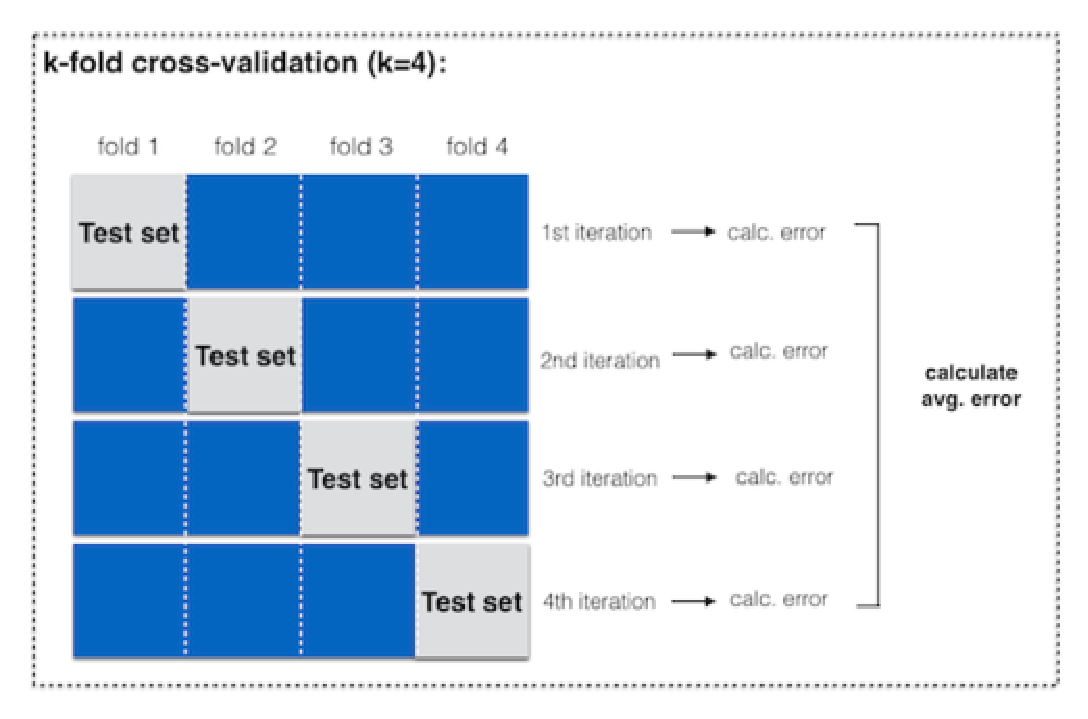
\includegraphics[width=0.6\textwidth,height=7cm]{figures/4-cv.eps}\\
  \caption{四折交叉验证}\label{fig:4-cv}
\end{figure}

\subsection{留一交叉验证}
留一交叉验证方法(Leave-One-Out Cross Validation,记为LOO-CV)是K折交叉验证方法$K=N$时的一个特例,轮换使用一个样本作为验证数据,其他$N-1$个样本构成训练集,训练得到$N$个模型,并根据它们在相应验证样本上预测精度的均值衡量模型性能。LOO-CV 的缺点是计算成本高,但相比K-CV方法,存在两个优点:
\begin{itemize}
  \item 每一回合,几乎全部样本皆用于训练模型,与原始样本的分布比较接近,训练与评估结果都比较可信。
  \item 实验过程没有引入随机因素,实验过程完全可以重现,进行不同模型的比较分析。
\end{itemize}

\section{奥卡姆剃刀}
奥卡姆剃刀(Occam's Razor)原理是由14世纪逻辑学家、修士William of Occam提出的一种逻辑或者解决问题需要遵循的基本原则,可以归纳为一句话:在假设空间中,最简单的那个假设(朴素原则)应当优先考虑。比如,将奥卡姆剃刀原理应用到模型选择问题时,应当遵循的基本原则是“在所有可能选择的模型中,能够很好地解释已知数据且形式简单的模型才是最好的模型,应该优先考虑”\cite{li2012statlearning}。

\section{没有免费午餐定理}%No Free Lunch

\section{经验法则}%Rules of Thumb

\section{贪婪算法}%Greedy Algorithm

\section{在线机器学习}
在线机器学习(Online Machine Learning)算法属于一种归纳模型,每次迭代只学习一个样例。在线学习算法主要用于样本预测,如给定一组可以描述今天股票市场的样本,在线学习算法能够预测某支股票明天的价格。在线学习的典型特征是预测的即时性,一旦发现新的样本标记,便可使用它修正在线学习算法的模型假设,从而不断地改善预测模型的表现。感知器算法、Pegasos算法与Winnow算法是三个经典的在线学习算法。

一般地,在线学习算法是通过持续的试错学习实现逐步演化,每次试错学习都包含三个步骤:
\begin{itemize}
  \item 接收一个新的样例$x$
  \item 预测样例的标记$\tilde{y} = f(\omega,x)$
  \item 接收样例的真实标记$y$,更新模型$\omega$
\end{itemize}
第三步是最关键的一步,学习算法充分利用样例的真实标记调整、更新假设模型。在模型调整时,在线学习算法通常依赖于标准的性能指标,如均方差、错误分类的比例最小化等。只要保证新样本的不断出现,在线学习算法可以持续地学习与改善,稳定性高、可扩展性强。

\section{超参数优选}%Hyper-parameter Learning
标准的监督学习包括两个重要环节:在训练集与验证集上训练和选择模型,在测试集上测试模型。模型训练阶段,一般都涉及到参数优选过程。对于某些模型,存在一类称作\textbf{超参数}(Hyper-parameter)的特殊参数,在训练之前就需要指定,如KNN模型中的$K$,神经网络模型中的隐藏层层数和隐藏层节点个数等。超参数对于模型性能影响较大,常用的\textbf{超参数优选方法}是\textbf{交叉验证方法},下文以线性回归分析为例,介绍使用K折交叉验证方法优选超参数的基本流程。

线性回归分析的目标是最小化模型$f(x,\theta) = \theta^T x$在训练数据集$S_\textrm{Train}$上的经验风险损失
\begin{equation}
    L(S_\textrm{Train}, \theta, \lambda) = \frac{1}{2n_\textrm{train}} \sum\limits_{(x,y)\in S_\textrm{Train}} \big[y - f(x, \theta)\big]^2 + \lambda \theta^T \theta
\end{equation}
第一部分表示均方差项,第二部分表示正则化项,$\lambda>0$是正则化因子,属于超参数,限定选择范围$\{\lambda_1,\ldots,\lambda_m\}$。

\begin{enumerate}[Step 1. ]
  \item 将原始数据集按照一定比例分成$A$和$B$两部分,数据$B$ 作为测试集不参与模型训练与选择,在数据$A$上使用K折交叉验证选择合适的超参数。表
  \ref{tbl:fivefoldcv}是5折交叉验证数据:数据$A$等分成五份$S_1, S_2, S_3, S_4, S_5$,轮换使用一个子集作为验证集,其它子集作为训练集,产生五折交叉验证数据集
    \begin{table}[htbp]
    \caption{五折交叉验证数据集}
    \label{tbl:fivefoldcv}
    \centering
    \begin{tabular}{c|c|c}
      \hline
      Fold & 训练集 & 验证集\\
      \hline
      Fold1 & $S_2,S_3,S_4,S_5$ & $S_1$ \\
      Fold2 & $S_1,S_3,S_4,S_5$ & $S_2$ \\
      Fold3 & $S_1,S_2,S_4,S_5$ & $S_3$ \\
      Fold4 & $S_1,S_2,S_3,S_5$ & $S_4$ \\
      Fold5 & $S_1,S_2,S_3,S_4$ & $S_5$ \\
      \hline
    \end{tabular}
    \end{table}
  \item 选择超参数$\lambda_1$,通过最小化Fold1训练集$S_\textrm{Train}=\{S_2,S_3,S_4,S_5\}$上的经验风险损失函数训练模型
      \begin{equation}
        \theta_\textrm{Train}^1 = \argmin\limits_{\theta}~~L(S_\textrm{Train}, \theta, \lambda_1)
      \end{equation}
  \item 在Fold1中验证集$S_1$上计算模型的经验风险损失
   \begin{equation}
      L_{11} = L(S_\textrm{Vali}, \theta_\textrm{Train}^1, \lambda_1)
   \end{equation}
  \item 在其他折执行上两步,在对应折训练集上训练模型,并在对应验证集上评估模型的经验风险损失$L_{12},\ldots,L_{15}$,计算平均损失$L_1=\sum\limits_{i=1}^5 L_{1i}/5$。
  \item 对于每个超参数$\lambda_i$执行上述步骤,计算平均性能$L_i$,选择平均损失最小的超参数$\lambda^*$作为最佳超参数,并使用它在数据集$A$上训练模型,得到最优参数$\theta^*,\lambda^*$。
  \item 根据训练的模型,在测试集$B$上测试模型,计算模型的预测损失
  \begin{equation}
    \frac{1}{2n_\textrm{test}} \sum\limits_{(x,y)\in S_\textrm{Test}} \big[y - f(x, \theta^*)\big]^2
  \end{equation}
\end{enumerate}

使用交叉验证的方法优选超参数计算开销大,目前存在几种流行的近似优化方法,如网格搜索、随机搜索\cite{bergstra2012random}。根据\cite{bergstra2012random}实验结果,对于含有多个超参数的模型,随机搜索远比网格搜索效率高而且效果更佳。Metzler和Croft\cite{metzler2007linear}使用一种监督学习的方法进行参数优化。他们认为直接优化线性模型标准度量方式(如MAP,P@10),可以通过网格搜索或坐标上升算法予以解决。由于标准度量模型是非平滑,直接优化标准度量,传统的优化算法无能为力。他们认为,在高维空间,搜索标准度量的最大值点十分困难,但是如果能够选取合适的细粒度(Granularity),网格搜索算法就可以找到全局最大值点;坐标上升算法属于局部搜索方法,在标准度量为凹函数时,无法保证找到全局最大值点。如果标准度量包含多个局部最值点,可以通过重启动(restart)提高找到全局最优点的几率。Metzler 和Croft 在文中使用的就是坐标上升算法,每次搜索伴以10次随机重启(10 Random Restarts)。

\section{P/NP问题}
计算复杂度理论(Computational Complexity Theory)主要研究对象是计算机求解问题的速度,比如解决问题所需时间、内存空间、处理器等资源。复杂度理论将所有可以在\textbf{多项式时间}(Polynomial Time)内解决的问题划分为\textbf{P问题}。对于一个问题$S$,如果存在算法$A$,可以在$n^k$时间内解决问题$S$或者说它的时间复杂度是$O(n^k)$,其中$n$是输入大小,$k$是一个自然数,则$S$存在一个多项式时间算法。我们提供给算法$A$一个问题的可能答案,如果算法可以在多项式时间内验证此解正确与否,那么算法$A$ 就是一个\textbf{不确定性算法}(Nondeterministic Algorithm)。所有使用不确定算法在多项式时间内可以解决的问题统称\textbf{NP 问题},它可以在多项式时间内得到验证。由此可知,P 问题是NP问题的一个子集,即P$\subseteq$NP。如果一个NP问题的所有可能答案,都可以在多项式时间内进行正确与否的验证,则称它为\textbf{NP完全问题}(NP-Complete Problem, NPC)。

\begin{example}[子集加和问题]
给定一个整数集合,它的一个非空子集的所有元素加和是否等于零?比如集合$\{-2, -3, 15, 14, 7, -10\}$,我们可以迅速地给出肯定的答复,但是不存在一个多项式时间复杂度的算法构造一个加和为零的子集。子集加和问题是一个典型的NP问题,但不一定是P问题。
\end{example}

2000年,美国Clay数学研究所(Clay Mathematics Institute, CMI)收录七个千禧年数学难题,每个奖金一百万美元,排在第一问的是\textbf{P 对NP 问题}(P v.s. NP Problem)
\[P\stackrel{?}{=} \mathrm{NP}.\]
它是由著名计算机科学家、1982年度图灵奖得主Stephen A. Cook\cite{cook1971complexity}在1971年发现并提出的一个难题。它的意思是:对于任意一个问题,如果它的解可以使用计算机\textbf{迅速}(多项式时间)验证,这个问题是否同样可以使用计算机\textbf{迅速}求解。
Cook举了一个有趣的例子形象地解释它:在一个周六的晚上,你参加了一个盛大的晚会,感到局促不安,你想知道大厅里是否有你认识的人。晚会的主人道:“你一定认识那位正在甜点盘附近的女士罗丝”。你只需向主人所指的方向扫一眼,也许发现他/她是正确的。如果缺少这样的暗示,你需要环顾整个大厅,一个个地审视。生成问题的一个解通常比验证给定的一个解所花费的时间多得多。

\section{收敛速度与复杂度}
假设数值迭代算法生成的序列为$\{x_k\}$,若序列收敛并且等式
\begin{equation}
    \hat x = \lim\limits_{k\rightarrow \infty} x_k
\end{equation}
成立。如果存在$\mu\ge 0$,使得
\begin{equation}
    \mu = \lim\limits_{k\rightarrow \infty} \frac{\|x_{k+1} - \hat x\|}{\|x_k - \hat x\|}
\end{equation}
则$\mu$称为序列$\{x_k\}$的\textbf{收敛速率}(Convergence Rate)。如果$\mu\in(0,1)$,则称序列\textbf{线性收敛};如果$\mu=0$,则称序列\textbf{超线性收敛};如果$\mu=1$,则称序列\textbf{次线性收敛}。
如果序列次线性收敛,并且满足下式:
\begin{equation}
    \lim\limits_{k\rightarrow \infty} \frac{\|x_{k+2} - x_{k+1}\|}{\|x_{k+1}-x_k \|} = 1
\end{equation}
则称序列\textbf{对数收敛}至$\hat x$。

为了对超线性收敛细分,定义$q$-阶收敛速率
\begin{equation}
    \mu = \lim\limits_{k\rightarrow \infty} \frac{\|x_{k+1} - \hat x\|}{\|x_k - \hat x\|^q} >0
\end{equation}
其中,阶数$q>1$。当$q=2$时,则称序列\textbf{二阶收敛}。

在表示算法时空复杂度时,通常在渐进表示法(Asymptotic Notation)中使用$\mathcal O$表示渐进上界(最坏表现),$\Omega$ 表示渐进下界(最佳表现),$\Theta$ 表示是一种相对比较精确的方法。在实际应用中,以$\mathcal O$使用最为常见。

\section{适定问题与非适定问题}
1902年,法国数学家Jacques Hadamard\cite{hadamard1902problemes}在研究偏微分方程时提出适定问题(well-posed problem),认为所有刻画物理现象的数学模型都应该是适定的,即数学模型的解满足:存在性、唯一性和稳定性(模型解对初值变化连续)。在实际问题中,Hadamard意义下的适定条件并不通用,它无法解释部分模型对于数据微小扰动的敏感性,引发解的剧烈变化。如果数学模型只满足部分条件,就称作不适定问题(ill-posed problem),或模型不适定。比如,图像处理中遇到的不适定问题有:去噪(De-nosing)、复原(Restorsion)、放大(Zooming)、修补(Inpainting)、去马赛克(Demosaicing)、超分辨(Super-resolution)等。

解决不适定问题的方法有很多,其中一个最常使用的方法是Tikhonov 正则化,通过限定假设空间将原问题转化为适定问题。在统计学中,Tikhonov正则化方法应用于线性回归分析,称为岭回归。

\section{欠定系统与超定系统}
当线性方程组中未知数的数目大于方程的数目,则称线性系统\textbf{欠定}(Under Determined),反之则称线性系统\textbf{超定}(Over Determined)。如果线性方程系统没有解,则称它是具有\textbf{非一致性}(Inconsistent)线性方程系统。根据Rouch\'{e}–Capelli定理,当线性方程组增广矩阵的秩与系数矩阵的秩相对,则线性方程组存在唯一解;当增广矩阵的秩大于系数矩阵的秩时,则线性方程组无界;否则,它有无穷多解。欠定系统要么存在无穷多解,要么没有解。
